%% QADF-Net: Quality-Aware Spatial Dual-View Fusion for Diabetic Retinopathy Grading
%% Journal: Computerized Medical Imaging and Graphics (Elsevier)
%% Class options: for a single-column review copy use
%%   \documentclass[preprint,12pt,authoryear]{elsarticle}  (and enable \linenumbers below)
\documentclass[final,5p,times,twocolumn,authoryear]{elsarticle}
%%---------------------------------------------------------------
%% Packages
%%---------------------------------------------------------------
\usepackage{amsmath,amssymb,amsthm}
\usepackage{booktabs}
\usepackage{graphicx}
\usepackage{adjustbox}
\usepackage{xcolor}
\usepackage{hyperref}
\usepackage[expansion=false]{microtype}
\usepackage{multirow}
\usepackage{array}
\usepackage{lineno}

%%---------------------------------------------------------------
%% Macros
%%---------------------------------------------------------------
\newcommand{\qadfnet}{QADF-Net}
\newcommand{\qcsca}{QC-SCA}
\newcommand{\Attn}[1]{\operatorname{Attn}_{1\leftarrow 2}^{(#1)}}

\theoremstyle{plain}
\newtheorem{lemma}{Lemma}
\theoremstyle{remark}
\newtheorem{remark}{Remark}

\journal{Computerized Medical Imaging and Graphics}
%\linenumbers

%%=================================================================
\begin{document}
%%=================================================================

\begin{frontmatter}

\title{QADF-Net: Quality-Aware Spatial Dual-View Fusion for Diabetic
  Retinopathy Grading under Quality Asymmetry}

\author[a1]{Quoc Thai Mai\corref{cor1}}
\ead{23133071@student.hcmute.edu.vn}
\author[a1]{Thanh Tuan Nguyen}
\author[a1]{Thi-The Phan}

\cortext[cor1]{Corresponding author.}

\affiliation[a1]{%
  organization={Faculty of Information Technology,
    Ho Chi Minh City University of Technology and Engineering (HCMUTE)},
  addressline={01 Vo Van Ngan Street, Thu Duc City},
  city={Ho Chi Minh City},
  country={Vietnam}
}

%%-----------------------------------------------------------------
%% Abstract  (<=250 words)
%%-----------------------------------------------------------------
\begin{abstract}
Dual-view diabetic retinopathy (DR) grading combines macula- and disc-centred fundus photographs, but fusion operators assume similar quality in both views. When one view is degraded, fusion can be worse than using the clearer view alone. We propose QADF-Net, in which a frozen lightweight estimator supplies per-view quality scores to a quality-conditioned spatial cross-attention (QC-SCA). A per-image quality bias on attention logits is cancelled by the softmax; a learnable sink token with a zero value vector makes it effective, and quality-proportional value scaling shrinks messages from low-quality views; a CORAL head preserves grade ordering. On DeepDRiD (200 test pairs, five seeds), QADF-Net matches the strongest baselines on clean images (quadratic weighted kappa 0.8805). Across seven degradation types at five severities with analytic quality scores, it obtained the highest mean area under the degradation curve (AUDC, 0.8666), significantly above Average and Concat after Holm correction; quality-weighted pooling without attention (0.8584) captured about half of its gain over standard cross-attention. Its Harm Rate, the share of pairs in which fusion errs more than a fixed, quality-selected single-view reference, rose by 2.2 percentage points from clean to the most severe level, versus 5.8--16.3 points for five other operators. With scores estimated online from degraded images, it again ranked first among five methods (AUDC 0.8662; Harm Rate 14.63\% at the most severe level), within seed variability of quality-weighted pooling. The advantage appeared only at moderate to high severity, not on natural pairs. The module adds 0.13 M parameters and 1.7 ms per pair.
\end{abstract}

%%-----------------------------------------------------------------
%% Graphical Abstract (min 531 x 1328 px, 300 dpi, <=8 MB)
%%-----------------------------------------------------------------
%% Graphical abstract is optional; uncomment once the image file is available.
%% (An empty graphicalabstract environment would typeset an empty block.)
%\begin{graphicalabstract}
%  \includegraphics{figures/graphical_abstract.pdf}
%\end{graphicalabstract}

%%-----------------------------------------------------------------
%% Research Highlights (3--5 bullet points, each <=85 characters)
%%-----------------------------------------------------------------
\begin{highlights}
\item A per-image quality bias on attention logits is a softmax no-op.
\item A quality logit bias takes effect only with a zero-value sink token.
\item Harm Rate, flip rate and feature drift audit dual-view fusion safety.
\item Smallest Harm Rate growth also with online quality estimates.
\item No detectable clean-image cost; 0.13 M parameters and 1.7 ms added.
\end{highlights}

%%-----------------------------------------------------------------
%% Keywords
%%-----------------------------------------------------------------
\begin{keyword}
diabetic retinopathy grading \sep
dual-view fundus image analysis \sep
quality-aware multi-view fusion \sep
cross-view feature contamination \sep
quality-conditioned cross-attention \sep
computer-aided diagnosis
\end{keyword}

\end{frontmatter}

%%=================================================================
%%  SECTION 1 --- INTRODUCTION
%%=================================================================
\section{Introduction}
\label{sec:intro}

Diabetic retinopathy (DR) is a microvascular complication of diabetes mellitus and one of the leading causes of preventable and, once advanced, irreversible visual impairment in working-age adults \citep{Cheung2010}. Global projections indicate that the number of people living with DR will approach 160 million by 2045 \citep{Teo2021}, a burden that places heavy demands on screening services and on the ophthalmic workforce. Colour fundus photography is the principal imaging modality for population-level screening, and deep learning has transformed automated DR grading since the first clinically validated systems \citep{Gulshan2016,Ting2017} and their extension across the disease spectrum \citep{Dai2021}. More recently, architectures that combine convolutional and self-attention mechanisms have pushed performance further; examples published in this journal include the CNN--Transformer fusion network of \citet{Huang2025drctfn} for DR image classification and the uncertainty-guided, semi-supervised Transformer--CNN framework of \citet{Malik2026uncertainty} for multiclass eye-disease classification. Most of these systems, however, reason about a single photograph per eye, whereas clinical practice relies on more than one view.

In line with the multi-field ETDRS tradition \citep{ETDRS1991report10}, a thorough fundus examination acquires at least two complementary fields: a \emph{macula-centred} image, in which microaneurysms, small haemorrhages, exudates and macular oedema are best visible, and an \emph{optic-disc-centred} image, which better exposes neovascularisation at or near the optic disc. Multi-view and dual-view networks have reported that fusing these fields improves grading over single-view baselines \citep{Zhao2019multiview,Sun2021dualview,Wang2021mvdr}, and recent work refines multi-view fusion with transformers, dynamic view selection and graph-based fusion \citep{Luo2025dynsel,Li2026mvgfdr}. The DeepDRiD challenge dataset \citep{Liu2022deepdrid}, which provides paired macula- and disc-centred images together with expert annotations of image quality, has made this dual-view setting a public benchmark.

A practical assumption behind many dual-view fusion methods is that \emph{both} views are of comparable optical quality. This rarely holds in the clinic. Cataract, patient motion, small or unevenly dilated pupils and operator variability regularly produce examinations in which one view is sharp while the other is blurred, over-exposed or too dark. Evidence from real-world screening shows that quality is a first-order concern: \citet{Pinto2026riqmonitor} analysed 55{,}801 retinal images from a DR screening programme and showed that continuous quality scores, decomposed into artefact- and opacity-related components, can monitor acquisition quality and guide improvements of imaging protocols. We call the situation in which the two views of one examination differ markedly in quality \emph{quality asymmetry}. Under quality asymmetry, symmetric fusion operators (concatenation, averaging, max-pooling or standard cross-attention) can propagate corrupted features into the joint representation (\emph{feature contamination}). A dual-view system is hard to justify clinically if its output is often worse than that obtained from the clearer of its two views. We quantify this with the \emph{Harm Rate}: the proportion of test cases in which the fused prediction has a strictly larger absolute grade error than a single-view reference prediction taken from the view with the higher expert quality score (Section~\ref{sec:metrics}). In our controlled-degradation benchmark, the Harm Rate of naive concatenation reaches 28.79\% at the most severe level of asymmetric degradation.

Many multi-view fundus methods fuse global vectors obtained after global average pooling (GAP) or rely on unconstrained cross-attention. Global pooling collapses spatial dimensions and discards the layout of minute lesions (such as microaneurysms and small haemorrhages) and of localised optical artefacts (such as glare streaks or peripheral shadowing). Conversely, injecting quality into spatial cross-attention as an additive logit bias, e.g.\ $\beta\log q$, meets a simple but easily overlooked obstacle: when the bias is a per-image scalar added to all source tokens of the same view, the softmax is invariant to it and the attention weights are left \emph{exactly} unchanged (a ``softmax no-op''; Section~\ref{sec:qcsca}). The query view is then still forced to distribute its full attention mass over the degraded view.

We therefore propose \textbf{QADF-Net} (Quality-Aware Spatial Dual-View Fusion Network), which injects quality information into the spatial attention itself. A frozen lightweight quality estimator (MobileNetV3-Small; \citealp{Howard2019mobilenetv3}) predicts a score $q\in(0,1]$ for each view. The scores condition a \emph{Quality-Conditioned Spatial Cross-Attention} (QC-SCA) that operates on the $14\times14$ token grid of each view. QC-SCA augments the key--value set with a learnable \emph{sink token} whose value vector is fixed to zero ($v_{\text{sink}}\equiv\mathbf{0}$) and which does not receive the quality bias; as the source quality decreases, attention mass moves to the sink and the contribution of the corrupted view fades smoothly and differentiably. A quality-proportional scaling of the value projections (Scale-V) further contracts the cross-view message, and a CORAL ordinal head \citep{Cao2020coral} predicts the DR grade while respecting its ordinal structure.

The contributions of this work are as follows.  
\begin{itemize}
  \item \textbf{A mechanism for quality-conditioned spatial cross-attention.} We show why a per-image quality bias cannot influence softmax attention, and make the bias effective with a zero-value sink token that does not receive it. Together with Scale-V, this gives a closed-form factorisation of the cross-view message and a simple norm bound (Lemma~\ref{lem:1}). In an ablation that crosses the two factors, neither the bias alone nor the sink alone gives a clear gain, whereas the two together do (Section~\ref{sec:r_ablation}).
  \item \textbf{QADF-Net.} A dual-view DR grading network that combines this module with a frozen quality estimator and a CORAL head, with a small overhead (0.13\,M parameters and 1.7\,ms per pair over average pooling on the same backbone).
  \item \textbf{A controlled-degradation protocol with safety-oriented measures.} We evaluate seven degradation types at five severity levels and three view scenarios, and report Harm Rate, Help Rate, Prediction Flip Rate (PFR) and Feature Drift Index (FDI) alongside agreement and robustness measures, with patient-clustered statistics. Quality scores are supplied either analytically, to isolate the fusion mechanism, or by the frozen estimator applied to the degraded images (end-to-end).
  \item \textbf{An empirical study on DeepDRiD with an explicit statement of scope.} QADF-Net is on par with the strongest fusion baselines on clean images and shows the smallest growth of Harm Rate, flip rate and feature drift as one view degrades when the quality scores are supplied analytically; an end-to-end evaluation in which the frozen estimator is applied to the degraded images gives the same AUDC ranking of the five methods reported (Section~\ref{sec:r_online_fq}). We also report where the advantage is absent: at low severity, on natural pairs and against some baselines on AUDC. A quality-weighted pooling baseline without attention captures about half of the AUDC gain of \qadfnet{} over standard cross-attention, so the added value of spatial attention over simple quality weighting is modest on these data under both quality protocols.
\end{itemize}

The remainder of the paper is organised as follows. Section~\ref{sec:related} reviews related work. Section~\ref{sec:method} presents QADF-Net. Section~\ref{sec:experiments} describes the dataset, baselines, metrics and degradation protocol. Section~\ref{sec:results} reports the results. Section~\ref{sec:discussion} discusses their implications and limitations, and Section~\ref{sec:conclusion} concludes.

%%=================================================================
%%  SECTION 2 --- RELATED WORK
%%=================================================================
\section{Related Work}
\label{sec:related}

\subsection{Automated diabetic retinopathy grading}
\label{sec:rw-dr}

Deep convolutional networks established automated DR detection as clinically viable, with validated sensitivity and specificity on large retrospective cohorts \citep{Gulshan2016,Gargeya2017}, across multi-ethnic populations \citep{Ting2017} and over a broader disease spectrum \citep{Dai2021}. Later work moved from purely convolutional backbones towards hybrid CNN--Transformer designs that combine local texture modelling with long-range context. Within this journal, \citet{Huang2025drctfn} proposed a CNN--Transformer fusion network for DR image classification, and \citet{Malik2026uncertainty} introduced a Transformer--CNN framework for multiclass eye-disease classification that uses Monte Carlo dropout uncertainty to refine pseudo-labels in a semi-supervised setting. Uncertainty has also been used earlier in DR detection to decide which cases to refer for expert review \citep{Leibig2017uncertainty}. These models are evaluated mostly on one image per eye of adequate quality.

DR severity is an ordered scale (grade~0 to grade~4), so the training objective matters. Cross-entropy treats all misclassifications alike, whereas confusing grade~0 with grade~4 is clinically worse than confusing it with grade~1. Ordinal-regression formulations decompose the $K$-class problem into $K-1$ cumulative binary tasks. CORAL \citep{Cao2020coral} enforces rank consistency by sharing one weight vector across tasks and learning task-specific biases, which yields parallel decision thresholds and monotonic cumulative probabilities; a later extension models conditional probabilities of the rank tasks \citep{Shi2022coral}. We adopt a CORAL head.

\subsection{Multi-view and dual-view fundus analysis}
\label{sec:rw-multiview}

The clinical protocol for DR assessment, rooted in the ETDRS standard, relies on multiple retinal fields \citep{ETDRS1991report10}. Computational counterparts include a dual-view collaborative network \citep{Zhao2019multiview}, a multi-view fundus grading network \citep{Sun2021dualview} and the fusion of fundus photographs with OCT volumes \citep{Wang2021mvdr}. More recent approaches explore richer fusion: \citet{Luo2025dynsel} select informative tokens across views and fuse view-level features with a mixture-of-experts module that strengthens key views and attenuates conflicting ones, and \citet{Li2026mvgfdr} fuse multi-view graphs that separate shared and view-specific information, evaluated on the multi-view fundus dataset MFIDDR. DeepDRiD \citep{Liu2022deepdrid} provides a public benchmark with paired macula- and disc-centred images. A distinct line of work concerns geometric alignment of fundus photographs; for example, \citet{Yan2025fundusreg} proposed a training-free two-stage colour fundus registration framework that refines SuperPoint/SuperGlue matches. Registration concerns \emph{where} content corresponds, not \emph{how reliable} each view is.

In the fusion methods we reviewed, the contribution of each view is determined by the image content and the learned fusion operator rather than by an explicit per-view quality estimate, and robustness under controlled quality asymmetry is not evaluated. When one view is degraded, no dedicated mechanism prevents its features from entering the joint representation. Our work targets this gap.

\subsection{Fundus image quality and quality-aware fusion}
\label{sec:rw-fiqa}

The EyeQ benchmark \citep{Shen2020eyeq} provides three-level quality grades (good, usable, reject) and is a standard resource for training retinal image quality estimators. DeepDRiD \citep{Liu2022deepdrid} complements it with expert quality annotations along several independent axes (clarity, field definition and artefacts) together with the DR grade, so that quality and diagnosis are available for the same images. Recent work moves from accept/reject decisions to continuous, interpretable scores: FundaQ-8 defines an eight-attribute, expert-validated framework and regresses a continuous score between 0 and 1, reporting improved diagnostic robustness when it is used in DR grading models \citep{Zun2025fundaq8}; NaIA-RD combines DR grading and retinal image quality grading in one screening system \citep{Pinto2025naia}. In real-world screening, \citet{Pinto2026riqmonitor} compared several quality models, including ones trained on EyeQ and DeepDRiD, against clinical decisions on 55{,}801 images. Most quality-assessment work treats the score as a \emph{filtering} or monitoring signal at the image level. We instead use it as a continuous control signal inside the fusion module, so that a partially degraded view can still contribute where it is informative.

Fusion of heterogeneous or redundant inputs has been surveyed extensively \citep{Baltrusaitis2018,Su2019multiview}. A common way to handle inputs of unequal reliability is to weight them by an estimated confidence; Bayesian formulations, for example, estimate aleatoric and epistemic uncertainty so that unreliable predictions can be down-weighted \citep{Kendall2017}. Weighting of this kind typically acts on pooled, one-dimensional summaries of each input or on final predictions, where a local degradation (a glare streak at the image border, peripheral under-exposure) cannot be separated from intact lesion regions. This motivates a \emph{spatial} formulation in which quality acts directly on token-level cross-attention. Quality-weighted pooling is the simplest pooled-level instance of such weighting; we include it both as a baseline (Section~\ref{sec:baselines}) and as an attention-free ablation (Section~\ref{sec:r_ablation}), so that the contribution of spatial attention can be separated from that of quality weighting itself.

\subsection{Cross-attention and attention sinks}
\label{sec:rw-attention}

Transformers \citep{Vaswani2017} and Vision Transformers \citep{Dosovitskiy2021} model dependencies through scaled dot-product attention, and co-attention or cross-attention variants are widely used to exchange information between two streams \citep{Lu2019coattn,Tsai2019multimodal}. Because softmax weights must sum to one, a query must distribute all of its attention mass over the available keys even when none of them is informative. Attention sinks were first described in streaming language models, where a few initial tokens absorb surplus attention \citep{Xiao2023sink}, and high-norm artefact tokens in Vision Transformers can be handled by extra \emph{register} tokens that provide a dedicated place for global computation \citep{Zhai2023registers}. In both cases the sink arises or is added to stabilise attention. We use the same idea for a different purpose: an explicit, learnable key paired with a \emph{zero value vector} that lets a query withdraw attention from an unreliable source view, with the amount of withdrawal controlled by an external quality score (Section~\ref{sec:qcsca}). Zero-value ``null'' attention targets or dustbins have been used before in other settings to absorb unmatched features or reject uninformative candidates \citep[e.g.,][]{Sukhbaatar2015memory,Sarlin2020superglue}, so we do not claim the sink itself as new; our contribution is its use together with a quality-dependent logit bias, and its evaluation as a safety mechanism for dual-view fundus fusion.

%%=================================================================
%%  SECTION 3 --- METHOD
%%=================================================================
\section{Method}
\label{sec:method}

Section~\ref{sec:overview} gives an overview of the three-stage pipeline, Section~\ref{sec:qest} describes the quality estimator, Section~\ref{sec:qcsca} details QC-SCA, Section~\ref{sec:prop1} analyses the message it delivers, and Section~\ref{sec:training} presents the CORAL head and the training protocol.

\subsection{Framework overview}
\label{sec:overview}

The network receives a pair of co-acquired fundus photographs of the same eye: a macula-centred view $I_1 \in \mathbb{R}^{3 \times H_0 \times W_0}$ and an optic-disc-centred view $I_2 \in \mathbb{R}^{3 \times H_0 \times W_0}$ ($H_0 = W_0 = 448$). Fig.~\ref{fig:pipeline} shows the three stages, and \ref{app:notation} lists the notation.

\begin{figure*}[htbp]
\centering
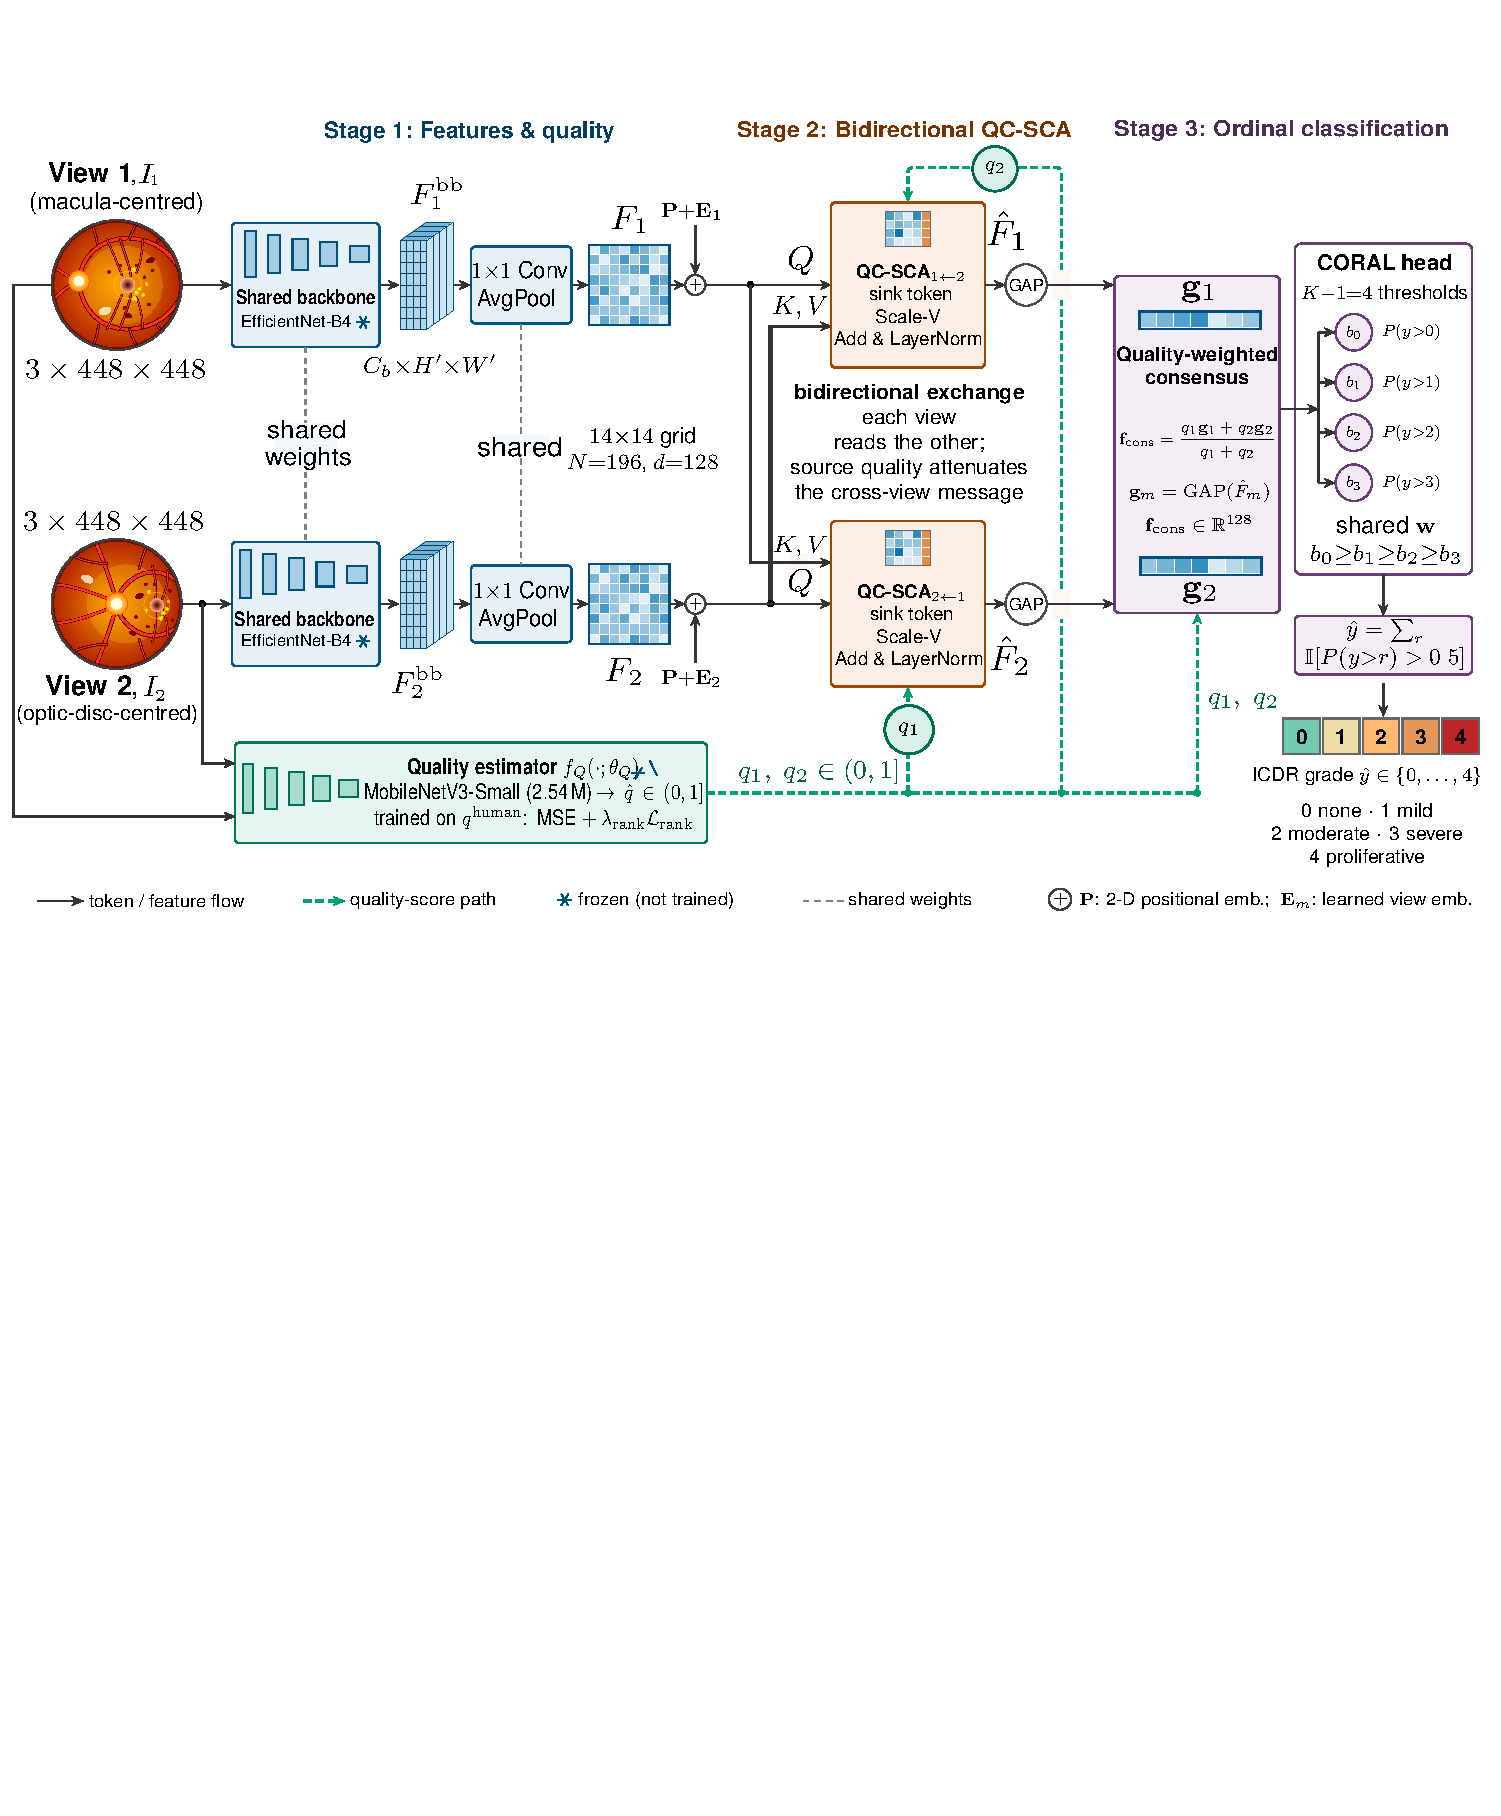
\includegraphics[width=\textwidth]{figures/fig1_architecture.pdf}
\caption{Architecture of \qadfnet{}. Co-acquired macula-centred and optic-disc-centred fundus photographs are mapped by a shared backbone to spatial token grids ($14 \times 14$). The frozen quality estimator produces scalar quality scores $q_1, q_2$. Bidirectional Quality-Conditioned Spatial Cross-Attention (\qcsca{}) uses a sink token ($\tau_{\text{sink}}$) and value-path scaling (Scale-V) so that the query view can draw on the complementary view while the contribution of a degraded view is attenuated. The consensus representation $\mathbf{f}_{\text{cons}}$ is classified by a rank-consistent CORAL ordinal head. Numerical values shown inside the panels are illustrative.}
\label{fig:pipeline}
\end{figure*}

\begin{enumerate}
  \item \textbf{Stage 1: spatial features and quality scores.} Each view $I_m$ ($m \in \{1, 2\}$) is processed by a shared backbone (EfficientNet-B4 \citep{Tan2019efficientnet} by default; ConvNeXt-Tiny \citep{Liu2022convnext} and Swin-Tiny \citep{Liu2021swin} are also evaluated) that is pretrained and kept frozen, giving feature maps $F_m^{\text{bb}} \in \mathbb{R}^{C_b \times H' \times W'}$ ($C_b = 1792$ for EfficientNet-B4). A shared $1{\times}1$ convolution and adaptive average pooling project each map onto a grid of $N = G \times G = 196$ tokens ($G = 14$) of dimension $d = 128$, giving $F_m \in \mathbb{R}^{N \times d}$ with tokens $\mathbf{f}_m^{(j)} \in \mathbb{R}^d$. A learned 2-D positional embedding and a view-specific embedding are added before fusion. Independently, a frozen lightweight estimator assigns each view a quality score $q_1, q_2 \in (0, 1]$.
  \item \textbf{Stage 2: bidirectional QC-SCA.} $F_1$ and $F_2$ attend to each other through two \qcsca{} modules conditioned on $q_1$ and $q_2$. Each uses a learned sink token with a zero value vector and a quality-dependent value scaling (Scale-V). The updated token sequences are pooled and combined by quality-weighted averaging into a consensus embedding $\mathbf{f}_{\text{cons}} \in \mathbb{R}^{d}$.
  \item \textbf{Stage 3: ordinal classification.} A CORAL head \citep{Cao2020coral} evaluates $K-1=4$ rank-ordered binary decisions to predict the ICDR grade $\hat{y} \in \{0, 1, 2, 3, 4\}$.
\end{enumerate}

\subsection{Quality score estimation}
\label{sec:qest}

DeepDRiD provides expert quality grades along three dimensions \citep{Liu2022deepdrid}: Image Clarity $C_{\text{img}} \in \{1, \dots, 10\}$, Field Definition $F_{\text{field}} \in \{1, \dots, 10\}$ and Artefact Severity $A_{\text{art}} \in \{0, \dots, 10\}$ (0 = no artefacts). We combine them into a normalised expert score
\begin{equation}
  q^{\text{human}} = \frac{C_{\text{img}} + F_{\text{field}} + (10 - A_{\text{art}})}{30} \in \left[\tfrac{2}{30}, 1\right],
  \label{eq:qhuman}
\end{equation}
which takes values in steps of $1/30$; higher values indicate better quality. The estimator $f_Q(\cdot;\theta_Q)$ is a MobileNetV3-Small \citep{Howard2019mobilenetv3} (2.54\,M parameters) that predicts a continuous $\hat{q} \in (0,1]$ from a single image. It is trained with
\begin{equation}
  \mathcal{L}_{\text{quality}} = \mathcal{L}_{\text{MSE}}(\hat{q}, q^{\text{human}}) + \lambda_{\text{rank}} \mathcal{L}_{\text{rank}}(\hat{q}, q^{\text{human}}),
  \label{eq:l_quality}
\end{equation}
where $\mathcal{L}_{\text{rank}}$ penalises pairwise inversions between images of different quality and $\lambda_{\text{rank}} = 0.5$. After training, $\theta_Q$ is frozen, so quality scores are deterministic and receive no gradient from the fusion loss.
The estimator is trained only on the training partition of the patient-level split of Section~\ref{sec:dataset}, and the validation partition is used to select the checkpoint with the lowest validation loss; no photograph from the test cohort is seen by $f_Q$ at any stage. Training uses AdamW (learning rate $5\times10^{-4}$, weight decay $10^{-4}$), a batch size of $16$ and $15$ epochs, with inputs resized to $224\times224$ pixels and ImageNet normalisation.
At inference \qadfnet{} supports three modes: \emph{learned} ($q_m = \hat{q}_m$; the deployable default), \emph{oracle} ($q_m = q_m^{\text{human}}$; a reference using expert annotations) and \emph{constant} ($q=1$; quality modulation disabled). How quality scores are supplied in the degradation benchmark, analytically or by $f_Q$ applied to the degraded images, is described in Section~\ref{sec:degradation}.

\subsection{Quality-conditioned spatial cross-attention (QC-SCA)}
\label{sec:qcsca}

Let $F_1, F_2 \in \mathbb{R}^{N \times d}$ be the token sequences of View~1 (queries) and View~2 (keys and values). For one head, learnable matrices $W_q, W_k, W_v \in \mathbb{R}^{d \times d_h}$, $d_h = d/H$, give $Q_1 = F_1 W_q$, $K_2 = F_2 W_k$ and $V_2 = F_2 W_v$. We use $H=4$ heads. Let $s^{0}_{ij} = Q_1^{(i)} (K_2^{(j)})^\top/\sqrt{d_h}$ denote the unbiased logit between query $i$ and key $j$.

\begin{remark}[Softmax invariance of a per-image quality bias]
\label{rem:noop}
Suppose quality is injected as an additive logit bias, $s_{ij} = s^{0}_{ij} + |\beta| \log q_2$. Because the bias is identical for every source token $j$, it cancels under the shift invariance of the softmax:
\begin{equation}
\begin{split}
  \frac{\exp(s_{ij}^{0} + |\beta| \log q_2)}{\sum_{k=1}^N \exp(s_{ik}^{0} + |\beta| \log q_2)}
  &= \frac{q_2^{|\beta|} \exp(s_{ij}^{0})}{q_2^{|\beta|} \sum_{k=1}^N \exp(s_{ik}^{0})} \\
  &= \frac{\exp(s_{ij}^{0})}{\sum_{k=1}^N \exp(s_{ik}^{0})}.
\end{split}
\end{equation}
The attention distribution is unaffected by $q_2$ (proof in \ref{app:noopproof}; illustrated analytically in Fig.~\ref{fig:softmax_noop}a). This is elementary, but it means that a per-image quality scalar cannot influence the attention weights through the logits alone.
\end{remark}

\begin{figure*}[!tb]
\centering
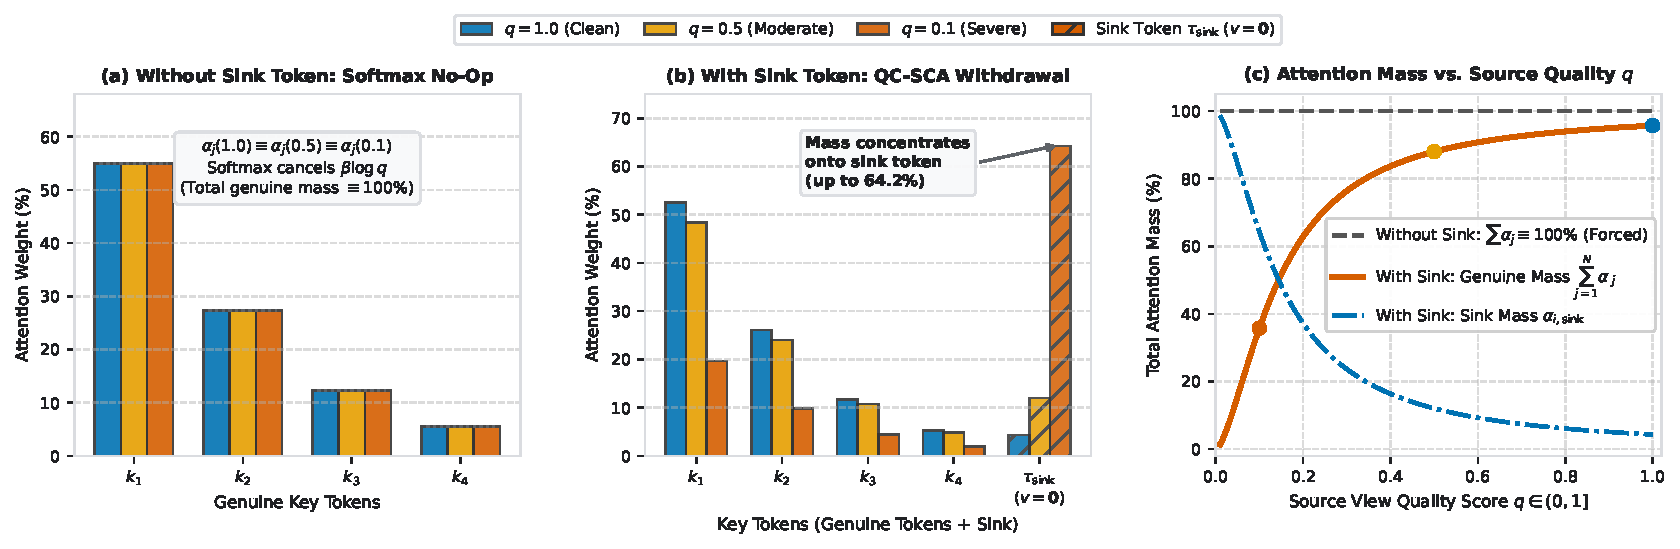
\includegraphics[width=\textwidth]{figures/fig_softmax_noop.pdf}
\caption{Analytical toy illustration of the softmax no-op phenomenon and the QC-SCA sink token mechanism (computed from closed-form formulas, not empirical data). (a)~Without a sink token, an additive per-image quality bias $\beta\log q_2$ applied to all source logits cancels under softmax shift invariance, leaving attention weights identical at $q \in \{1.0, 0.5, 0.1\}$ ($\alpha_j(q) \equiv \alpha_j(1.0)$) and forcing the query to distribute all attention mass over the degraded view. (b)~With a zero-value sink token $\tau_{\text{sink}}$ ($v_{\text{sink}} \equiv \mathbf{0}$) that does not receive the quality bias, decreasing quality causes attention mass on genuine tokens to contract while surplus mass routes smoothly to the sink. (c)~Total attention mass on genuine tokens versus continuous quality $q \in (0, 1]$: standard softmax remains invariant at $100\%$, whereas QC-SCA attenuates the effective cross-view message smoothly and differentiably towards zero as $q \to 0$.}
\label{fig:softmax_noop}
\end{figure*}

\paragraph{Sink token} To give the softmax somewhere else to put attention mass, we append a learnable sink token $\tau_{\text{sink}} = (k_{\text{sink}}, v_{\text{sink}})$ to the key--value sequence of View~2, with
\begin{equation}
  v_{\text{sink}} \equiv \mathbf{0} \in \mathbb{R}^{d_h}.
  \label{eq:v_sink_zero}
\end{equation}
The logits from query token $i$ to the $N+1$ candidates are
\begin{equation}
  \tilde{s}_{ij} =
  \begin{cases}
    s^{0}_{ij} + |\beta| \log(q_2 + \epsilon), & j \le N, \\[4pt]
    \dfrac{Q_1^{(i)} k_{\text{sink}}^\top}{\sqrt{d_h}}, & j = N+1 \ (\text{sink}),
  \end{cases}
  \label{eq:logits_qcsca}
\end{equation}
where $\beta$ is a learnable scale ($|\beta|$ keeps the bias non-positive for $q_2 \le 1$, apart from the negligible offset introduced by $\epsilon$) and $\epsilon = 10^{-6}$ ensures numerical stability. Since the bias is applied \emph{only} to genuine tokens, the cancellation in Remark~\ref{rem:noop} no longer occurs: as $q_2$ decreases, attention mass on genuine tokens contracts and routes smoothly into $\tau_{\text{sink}}$ (Fig.~\ref{fig:softmax_noop}b,c). When $q_2 \to 1$ the bias vanishes and the query distributes its attention between genuine tokens and the sink according to the learned logits; when $q_2 \to 0$ the genuine tokens' weights vanish and
\begin{equation}
\begin{gathered}
  \alpha_{i,\text{sink}} = \frac{\exp(\tilde{s}_{i,N+1})}{\exp(\tilde{s}_{i,N+1}) + \sum_{j=1}^N \exp(\tilde{s}_{ij})} \xrightarrow[q_2 \to 0]{} 1, \\
  \sum_{j=1}^N \alpha_{ij} \xrightarrow[q_2 \to 0]{} 0 .
\end{gathered}
\end{equation}

\paragraph{Scale-V} In addition, the value vectors of the source view are scaled by its quality:
\begin{equation}
  \tilde{V}_2^{(j)} = q_2 \, W_v \mathbf{f}_2^{(j)}, \quad j \in \{1, \dots, N\}.
  \label{eq:scale_v}
\end{equation}
The message delivered to query token $i$ is
\begin{equation}
  \Attn{i} = \sum_{j=1}^N \alpha_{ij} \tilde{V}_2^{(j)} + \alpha_{i,\text{sink}} v_{\text{sink}} = q_2 \sum_{j=1}^N \alpha_{ij}\, W_v \mathbf{f}_2^{(j)} ,
  \label{eq:attn_update}
\end{equation}
because $v_{\text{sink}} = \mathbf{0}$.

\paragraph{Bidirectional consensus} The operation is applied in both directions, $m_{1 \leftarrow 2} = \text{QC-SCA}(F_1, F_2, q_1, q_2)$ and $m_{2 \leftarrow 1} = \text{QC-SCA}(F_2, F_1, q_2, q_1)$, followed by residual connections and layer normalisation as in \citet{Vaswani2017}:
\begin{equation}
\begin{split}
  \hat{F}_1 &= \operatorname{LayerNorm}(F_1 + m_{1 \leftarrow 2} W_o),\\
  \hat{F}_2 &= \operatorname{LayerNorm}(F_2 + m_{2 \leftarrow 1} W_o),
\end{split}
\end{equation}
where $W_o \in \mathbb{R}^{d \times d}$ merges the heads. After GAP, the two vectors are combined by quality-weighted averaging:
\begin{equation}
  \mathbf{f}_{\text{cons}} = \frac{q_1}{q_1 + q_2}\operatorname{GAP}(\hat{F}_1) + \frac{q_2}{q_1 + q_2}\operatorname{GAP}(\hat{F}_2) \in \mathbb{R}^{d}.
  \label{eq:f_cons}
\end{equation}
Setting $q_1 = q_2$ recovers unweighted averaging. The internal dataflow of a single QC-SCA head is illustrated in Fig.~\ref{fig:qc_sca}.

\begin{figure*}[!tb]
\centering
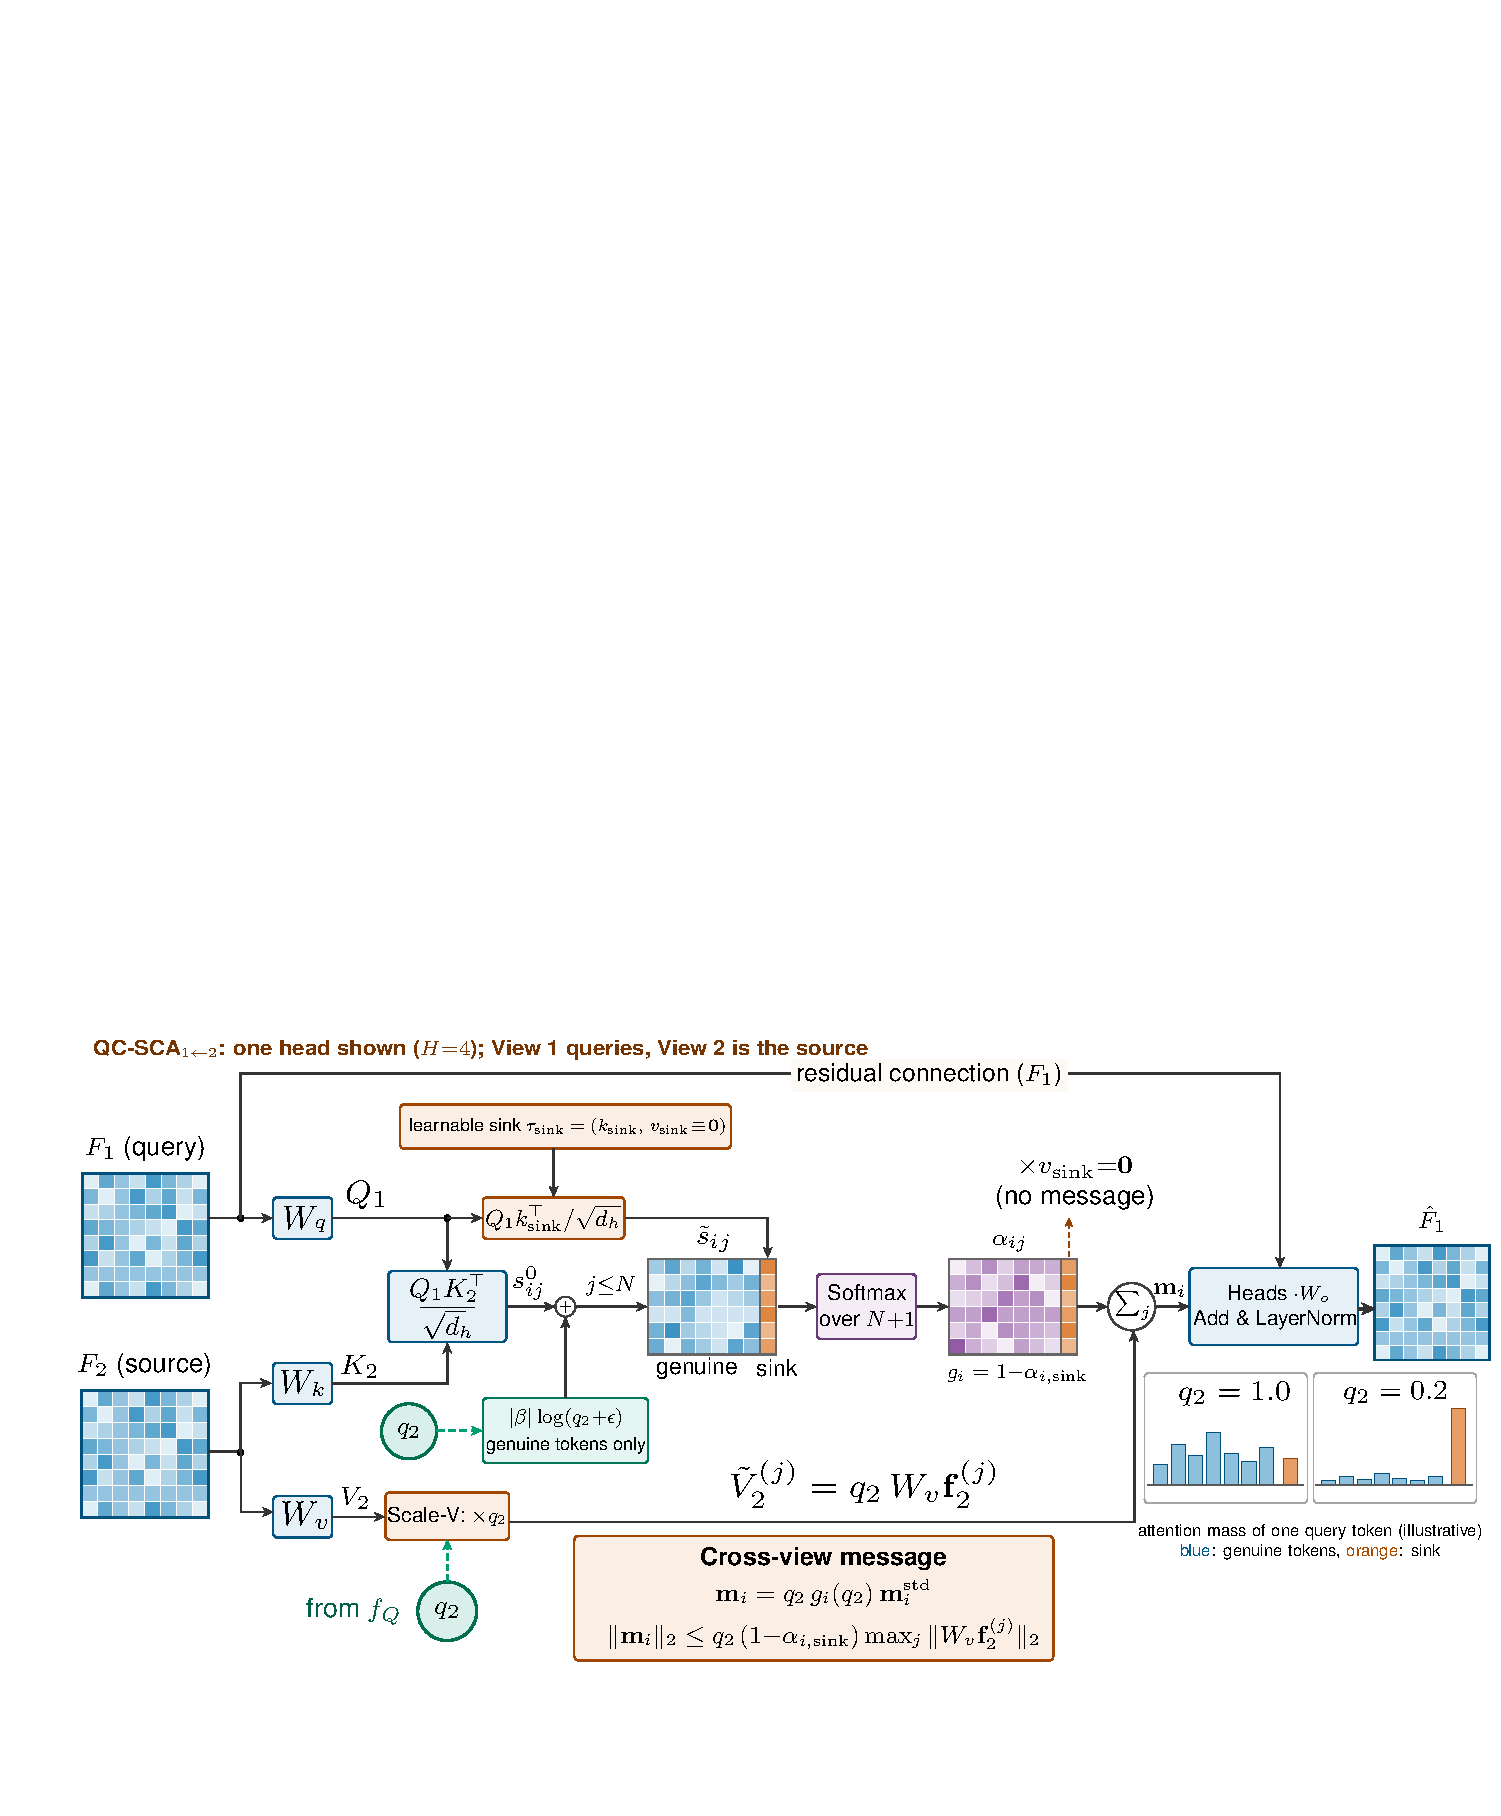
\includegraphics[width=\textwidth]{figures/qc_sca.pdf}
\caption{Detailed architectural schematic of a single Quality-Conditioned Spatial Cross-Attention (QC-SCA) head ($H=4$), with View~1 serving as queries ($F_1$) and View~2 as source ($F_2$). Genuine source tokens receive an additive logit bias $|\beta|\log(q_2+\epsilon)$, surplus attention mass routes smoothly into the zero-value sink token $\tau_{\text{sink}}$ ($v_{\text{sink}} \equiv \mathbf{0}$), and source value vectors are dynamically scaled by $q_2$ (Scale-V), ensuring that the delivered cross-view message $\mathbf{m}_i$ contracts smoothly towards zero as source quality degrades.}
\label{fig:qc_sca}
\end{figure*}

\subsection{Analysis of the cross-view message}
\label{sec:prop1}

Write $Z_i = \sum_{j=1}^N \exp(s_{ij}^{0})$ for the total affinity of query $i$ to the genuine tokens, $s_{i,\text{sink}}$ for its sink logit, $p_{ij} = \exp(s_{ij}^{0})/Z_i$ for the unmodulated attention weights and $\mathbf{m}_i^{\text{std}} = \sum_j p_{ij} W_v \mathbf{f}_2^{(j)}$ for the unmodulated message (the case $q_2 = 1$ without sink; $\epsilon$ is omitted for readability). Then $\alpha_{ij} = g_i(q_2)\,p_{ij}$ with
\begin{equation}
\begin{split}
  g_i(q_2) &= \frac{q_2^{|\beta|} Z_i}{\exp(s_{i,\text{sink}}) + q_2^{|\beta|} Z_i} \\
  &= \sigma\!\big(|\beta|\log q_2 + \log Z_i - s_{i,\text{sink}}\big) \\
  &= 1 - \alpha_{i,\text{sink}} \in (0,1),
\end{split}
\end{equation}
where $\sigma$ is the logistic function, and the message of Eq.~\eqref{eq:attn_update} factorises exactly as
\begin{equation}
  \Attn{i} = q_2\, g_i(q_2)\, \mathbf{m}_i^{\text{std}} .
  \label{eq:message_factorization}
\end{equation}
Scale-V thus contributes a query-independent factor $q_2$, and the sink contributes a query-dependent factor $g_i$ that is smaller for queries with low total affinity $Z_i$. In the regime $q_2^{|\beta|} Z_i \ll \exp(s_{i,\text{sink}})$, $g_i \approx q_2^{|\beta|} Z_i/\exp(s_{i,\text{sink}})$ and the compound factor scales as $q_2^{1+|\beta|}$. This regime is not the typical one in our experiments (for the representative pair of Fig.~\ref{fig:attn_maps} the mean $g_i$ is about $0.51$ at the most severe level; Section~\ref{sec:r_safety}).

\begin{lemma}[Norm bound on the cross-view message]
\label{lem:1}
For any query token $i$ and any value of the quality scores $(q_1,q_2)\in(0,1]^2$,
\begin{equation}
\begin{split}
  \|\Attn{i}\|_2 &\le q_2\,\bigl(1-\alpha_{i,\text{sink}}\bigr)\max_{1 \le j \le N} \|W_v \mathbf{f}_2^{(j)}\|_2 \\
  &\le q_2 \cdot \max_{1 \le j \le N} \|W_v \mathbf{f}_2^{(j)}\|_2 .
\end{split}
  \label{eq:lemma_bound}
\end{equation}
\end{lemma}
\begin{proof}
By Eq.~\eqref{eq:attn_update} and the triangle inequality, $\|\Attn{i}\|_2 \le q_2 \sum_{j=1}^N \alpha_{ij}\|W_v \mathbf{f}_2^{(j)}\|_2 \le q_2 \bigl(\sum_{j=1}^N \alpha_{ij}\bigr)\max_j\|W_v \mathbf{f}_2^{(j)}\|_2$. Since the weights over the $N+1$ candidates are non-negative and sum to one, $\sum_{j=1}^N \alpha_{ij} = 1-\alpha_{i,\text{sink}} \le 1$.
\end{proof}

\begin{remark}[Scope of the bound]
\label{rem:scope}
The lemma is deliberately modest. (i)~The second inequality follows from Scale-V alone and would hold without a sink; the sink adds the factor $1-\alpha_{i,\text{sink}} = g_i$, which our ablation indicates helps in practice but which the lemma does not quantify. (ii)~The bound concerns the \emph{message} $\Attn{i}$ received by View~1. It is not a bound on the displacement of the consensus vector $\mathbf{f}_{\text{cons}}$ under an arbitrary perturbation of $F_2$: a perturbation also changes the attention weights through the keys, it enters $\hat{F}_2$ directly through the residual connection (down-weighted only by the consensus weight $q_2/(q_1+q_2)$), and layer normalisation is not globally Lipschitz. We therefore assess the end-to-end effect empirically with the Feature Drift Index (Section~\ref{sec:r_safety}) and do not claim a worst-case guarantee. (iii)~The weights in Eq.~\eqref{eq:lemma_bound} refer to one head; the multi-head message is a linear function of the per-head messages through $W_o$.
\end{remark}

\subsection{CORAL ordinal classifier and training protocol}
\label{sec:training}

DR progresses along an ordered scale: Grade~0 (No DR), 1 (Mild NPDR), 2 (Moderate NPDR), 3 (Severe NPDR) and 4 (PDR). The consensus vector $\mathbf{f}_{\text{cons}}$ is passed to a CORAL head \citep{Cao2020coral}, which defines $K-1 = 4$ binary tasks for the thresholds $r \in \{0, 1, 2, 3\}$:
\begin{equation}
  P(y > r \mid \mathbf{f}_{\text{cons}}) = \sigma(\mathbf{w}^\top \mathbf{f}_{\text{cons}} + b_r),
  \label{eq:coral_prob}
\end{equation}
where $\mathbf{w} \in \mathbb{R}^{d}$ is shared across thresholds, $b_0 \ge b_1 \ge b_2 \ge b_3$ are learned biases enforced by a monotone parameterisation, and $\sigma(z) = (1 + e^{-z})^{-1}$. Sharing $\mathbf{w}$ keeps the decision hyperplanes parallel and prevents rank inversions $P(y > r+1) > P(y > r)$. With indicators $y^{(r)} = \mathbb{I}(y > r)$, the loss is the sum of binary cross-entropies,
\begin{multline}
  \mathcal{L}_{\text{CORAL}} = -\sum_{r=0}^{K-2} \Big[ y^{(r)} \log \sigma(\mathbf{w}^\top \mathbf{f}_{\text{cons}} + b_r) \\
  + (1 - y^{(r)}) \log\bigl(1 - \sigma(\mathbf{w}^\top \mathbf{f}_{\text{cons}} + b_r)\bigr) \Big],
  \label{eq:l_coral}
\end{multline}
and the predicted grade is the number of thresholds whose probability exceeds $0.5$:
\begin{equation}
  \hat{y} = \sum_{r=0}^{K-2} \mathbb{I}\left( \sigma(\mathbf{w}^\top \mathbf{f}_{\text{cons}} + b_r) > 0.5 \right) \in \{0, 1, 2, 3, 4\}.
  \label{eq:coral_predict}
\end{equation}

\paragraph{Implementation details} Models are implemented in PyTorch and trained on a single NVIDIA Tesla T4 GPU with automatic mixed precision (FP16). Inputs are resized to $448 \times 448$ pixels (bicubic), and contrast-limited adaptive histogram equalisation (CLAHE) is applied to the luminance channel in Lab colour space (clip limit 2.0, $8 \times 8$ grid). The training objective is $\mathcal{L}_{\text{CORAL}}$. We use AdamW with learning rate $3 \times 10^{-4}$, weight decay $10^{-4}$ and a cosine schedule over 60 epochs with a 5-epoch linear warm-up. The batch size is 8 pairs with gradient accumulation over 4 steps (effective batch of 32 pairs, i.e.\ 64 photographs). Augmentation comprises random resized cropping (scale $[0.75, 1.0]$, aspect ratio $[0.9, 1.1]$), horizontal and vertical flips ($p=0.5$), rotations up to $\pm 30^\circ$, colour jitter (brightness 0.3, contrast 0.35, saturation 0.25, hue 0.05) and random greyscale conversion ($p=0.1$). The patient-stratified validation split is used for learning-rate monitoring and model selection; at each epoch, models are evaluated on this split, and the checkpoint achieving the highest validation Quadratic Weighted Kappa ($\kappa_w$) across the 60 training epochs is saved for final testing. Main benchmark models are trained with five seeds (42--46) and ablation sweeps with three seeds (42--44). A full configuration table is given in \ref{app:config}.

%%=================================================================
%%  SECTION 4 --- EXPERIMENTAL SETUP
%%=================================================================
\section{Experimental Setup}
\label{sec:experiments}

\subsection{Dataset and patient-level partitioning}
\label{sec:dataset}

All experiments use the regular-fundus subset of the DeepDRiD challenge dataset \citep{Liu2022deepdrid}: 500 patients, each contributing one dual-view pair per eye, i.e.\ 1{,}000 pairs and 2{,}000 photographs. Each pair consists of a macula-centred (Field~1) and an optic-disc-centred (Field~2) photograph and carries an ICDR grade assigned by certified retinal specialists: Grade~0 ($n=457$), 1 ($n=111$), 2 ($n=199$), 3 ($n=177$) and 4 ($n=56$). We use the official patient-level partition: 300 patients / 600 pairs for training, 100 patients / 200 pairs for validation and 100 patients / 200 pairs for testing. No patient appears in more than one subset (checked against the dataset manifest). The quality annotations (Section~\ref{sec:qest}) are used to derive $q^{\text{human}}$. All photographs are resized to $448\times448$ and preprocessed with CLAHE.

\subsection{Baseline fusion strategies}
\label{sec:baselines}

To isolate the contribution of \qcsca{}, we compare \qadfnet{} with nine baselines that share an identical protocol: the same frozen EfficientNet-B4 backbone (ConvNeXt-Tiny and Swin-Tiny are examined in Section~\ref{sec:r_backbone}), input resolution and CLAHE preprocessing, the same $1\times1$ projection and tokenisation to $\mathbb{R}^{N\times d}$ ($N=196$, $d=128$), the same CORAL head, augmentation pipeline and five seeds. Comparing with published end-to-end pipelines would confound the comparison through different backbones, resolutions, objectives and datasets; the baselines instead instantiate the fusion operators commonly used in dual-view work (single-view selection, global pooling operators, attention-based interaction \citep{Zhao2019multiview,Sun2021dualview,Wang2021mvdr,Lu2019coattn}). They fall into four groups.
\begin{enumerate}
  \item \textbf{Single-view references.} \emph{Single-View V1 (Macula)} and \emph{Single-View V2 (Optic Disc)} apply GAP to $F_1$ or $F_2$ and classify with the CORAL head. \emph{Best-Single (Quality Selector)} is a separately trained checkpoint with a selector that routes each pair to the view with the higher quality score ($q_1 \ge q_2 \Rightarrow$ View~1). On clean data the selector uses $q^{\text{human}}$ (privileged expert information), so it is an oracle single-view reference without cross-view fusion. Being a separate checkpoint, its results differ from those of V1 or V2 even when all pairs are routed to the same view.
  \item \textbf{Global fusion operators.} \emph{Concat} concatenates the pooled vectors $[p_1;p_2]\in\mathbb{R}^{2d}$ and projects back to $\mathbb{R}^d$; \emph{Average} computes $\tfrac12(p_1+p_2)$; \emph{Max} takes the element-wise maximum.
  \item \textbf{Quality-weighted pooling.} \emph{Q-Weighted GAP} drops cross-view interaction and combines the pooled vectors $p_m=\operatorname{GAP}(F_m)$ by the quality-weighted average of Eq.~\eqref{eq:f_cons}, $\mathbf{f}_{\text{cons}} = \tfrac{q_1}{q_1+q_2}\,p_1 + \tfrac{q_2}{q_1+q_2}\,p_2$. It receives the same quality scores as \qadfnet{} (learned $\hat q$; in the degradation benchmark the attenuated scores of Eq.~\eqref{eq:q_attenuation}, or the online estimates of $f_Q$ on the degraded images in Section~\ref{sec:r_online_fq}), and is therefore the closest quality-aware counterpart without spatial attention.
  \item \textbf{Attention-based operators.} \emph{Standard Cross-Attention} (Cross-Attn) is bidirectional spatial cross-attention on the $14\times14$ grids with the same multi-head architecture as \qcsca{} but $q\equiv1$ (no bias, no sink, no Scale-V, uniform consensus). \emph{Bilinear Co-Attention} (Co-Attn) \citep{Lu2019coattn,Kim2021coattn} concatenates the bilinear product of $p_1,p_2$ with their mean and projects to $\mathbb{R}^d$; it models cross-view interactions at the global level, without spatial resolution or quality conditioning.
\end{enumerate}
\emph{Quality information is used by three methods only:} \qadfnet{} and Q-Weighted GAP (learned $\hat q$ from $f_Q$) and Best-Single (oracle $q^{\text{human}}$). All other baselines receive no quality input. Hence the comparison asks how the proposed mechanism fares against quality-agnostic operators and against one simple quality-aware operator, and not against uncertainty-weighted or other learned quality-aware fusion (see the limitations in Section~\ref{sec:discussion}).

\subsection{Evaluation metrics}
\label{sec:metrics}

We evaluate diagnostic agreement, degradation robustness and clinical safety.

\paragraph{Diagnostic agreement} The primary measure is quadratic weighted kappa (QWK, $\kappa_w$) \citep{Cohen1968kappa},
\begin{equation}
  \kappa_w = 1 - \frac{\sum_{i,j} w_{ij} O_{ij}}{\sum_{i,j} w_{ij} E_{ij}}, \quad w_{ij} = \frac{(i - j)^2}{(K - 1)^2},
  \label{eq:qwk}
\end{equation}
with $O_{ij}$ and $E_{ij}$ the observed and chance-expected confusion matrices for $K=5$ grades. We also report accuracy and macro-averaged one-vs-rest AUC.

\paragraph{Robustness (AUDC)} For each degradation type the model is evaluated at severity levels $L \in \{0,\dots,5\}$ ($L=0$ clean). The Area Under the Degradation Curve is
\begin{equation}
  \text{AUDC} = \frac{1}{5} \sum_{L=0}^4 \frac{\kappa_w(L) + \kappa_w(L+1)}{2}.
  \label{eq:audc}
\end{equation}
The clean level therefore carries weight $0.1$; part of any AUDC gap reflects clean-image performance.

\paragraph{Clinical safety} Multi-view fusion is justified only if it does not produce worse decisions than the clearer single photograph. We define four measures.
\begin{enumerate}
  \item \textbf{Harm Rate:} the proportion of pairs in which the fused prediction has a strictly larger absolute error than the single-view reference prediction taken from the view with the higher expert quality score,
    \begin{equation}
      \text{Harm Rate} = \frac{1}{M} \sum_{i=1}^M \mathbb{I}\left( |\hat{y}_{\text{fus}}^{(i)} - y^{(i)}| > |\hat{y}_{\text{best\_view}}^{(i)} - y^{(i)}| \right),
      \label{eq:harm_rate}
    \end{equation}
    where $\hat{y}_{\text{best\_view}}^{(i)} = \hat{y}_{v1}^{(i)}$ if $q_1^{\text{human},(i)} \ge q_2^{\text{human},(i)}$ on the clean pair and $\hat{y}_{v2}^{(i)}$ otherwise. The reference view is selected without the disease label but with expert quality information, so it is a privileged reference; the selection is made once on the clean pair and held fixed across severity levels (Section~\ref{sec:r_safety}).
The prediction $\hat{y}_{\text{best\_view}}^{(i)}$ itself is likewise computed on the clean, uncorrupted photograph of the selected view and is never recomputed on degraded input, even when the selected view is the one being degraded. Harm Rate at $L \ge 1$ therefore measures the error of fusion relative to a fixed clean single-view decision, not relative to a single-view model that faces the same degraded photograph.
The single-view predictions come from the Single-View V1 and V2 models trained with the same seed and split.
  \item \textbf{Help Rate:} the proportion of pairs in which fusion has a strictly smaller error than the single-view reference,
    \begin{equation}
      \text{Help Rate} = \frac{1}{M} \sum_{i=1}^M \mathbb{I}\left( |\hat{y}_{\text{fus}}^{(i)} - y^{(i)}| < |\hat{y}_{\text{best\_view}}^{(i)} - y^{(i)}| \right).
      \label{eq:help_rate}
    \end{equation}
  \item \textbf{Prediction Flip Rate (PFR):} the frequency with which the predicted grade differs from the clean prediction,
    \begin{equation}
      \text{PFR}(L) = \frac{1}{M} \sum_{i=1}^M \mathbb{I}\left( \hat{y}^{(i)}(L) \neq \hat{y}^{(i)}(0) \right).
      \label{eq:pfr}
    \end{equation}
    A flip counts any change of grade, towards or away from the correct one, so PFR measures stability, not accuracy.
  \item \textbf{Feature Drift Index (FDI):} the normalised displacement of the consensus vector,
    \begin{equation}
      \text{FDI}(L) = \frac{\|\mathbf{f}_{\text{cons}}^{(L)} - \mathbf{f}_{\text{cons}}^{(0)}\|_2}{\|\mathbf{f}_{\text{cons}}^{(0)}\|_2}.
      \label{eq:fdi}
    \end{equation}
\end{enumerate}

\subsection{Controlled degradation benchmark}
\label{sec:degradation}

We construct a grid of seven degradation types at five severity levels ($L=1$ to $5$):
\begin{itemize}
  \item \textbf{Gaussian blur} (media opacity, e.g.\ cataract): $\sigma \in [1.0, 5.0]$.
  \item \textbf{Defocus blur} (refractive error, lens misalignment): disk kernels of radius $r \in [2, 14]$ pixels.
  \item \textbf{Motion blur} (patient motion, camera instability): linear kernels of length $\ell \in [5, 41]$ pixels.
  \item \textbf{Darkness} (inadequate flash, pupil constriction): gamma darkening $I^{\gamma}$, $\gamma \in [1.35, 3.70]$, with illumination attenuation down to $0.25$.
  \item \textbf{Glare} (corneal reflection): localised Gaussian highlight rings with radius ratios $18\%$--$48\%$ and peak intensities up to $0.95$.
  \item \textbf{JPEG compression} (low-bandwidth telemedicine): quality factors $Q \in [50, 4]$.
  \item \textbf{Occlusion} (eyelid droop, eyelashes): horizontal bands covering $10\%$ to $50\%$ of the vertical field.
\end{itemize}
Three view scenarios are evaluated for each type: (a)~View~2 degraded and View~1 clean (the canonical asymmetry); (b)~View~1 degraded and View~2 clean; (c)~both views degraded with the same severity. Fig.~\ref{fig:degrad} illustrates the seven types.

\begin{figure*}[!tb]
\centering
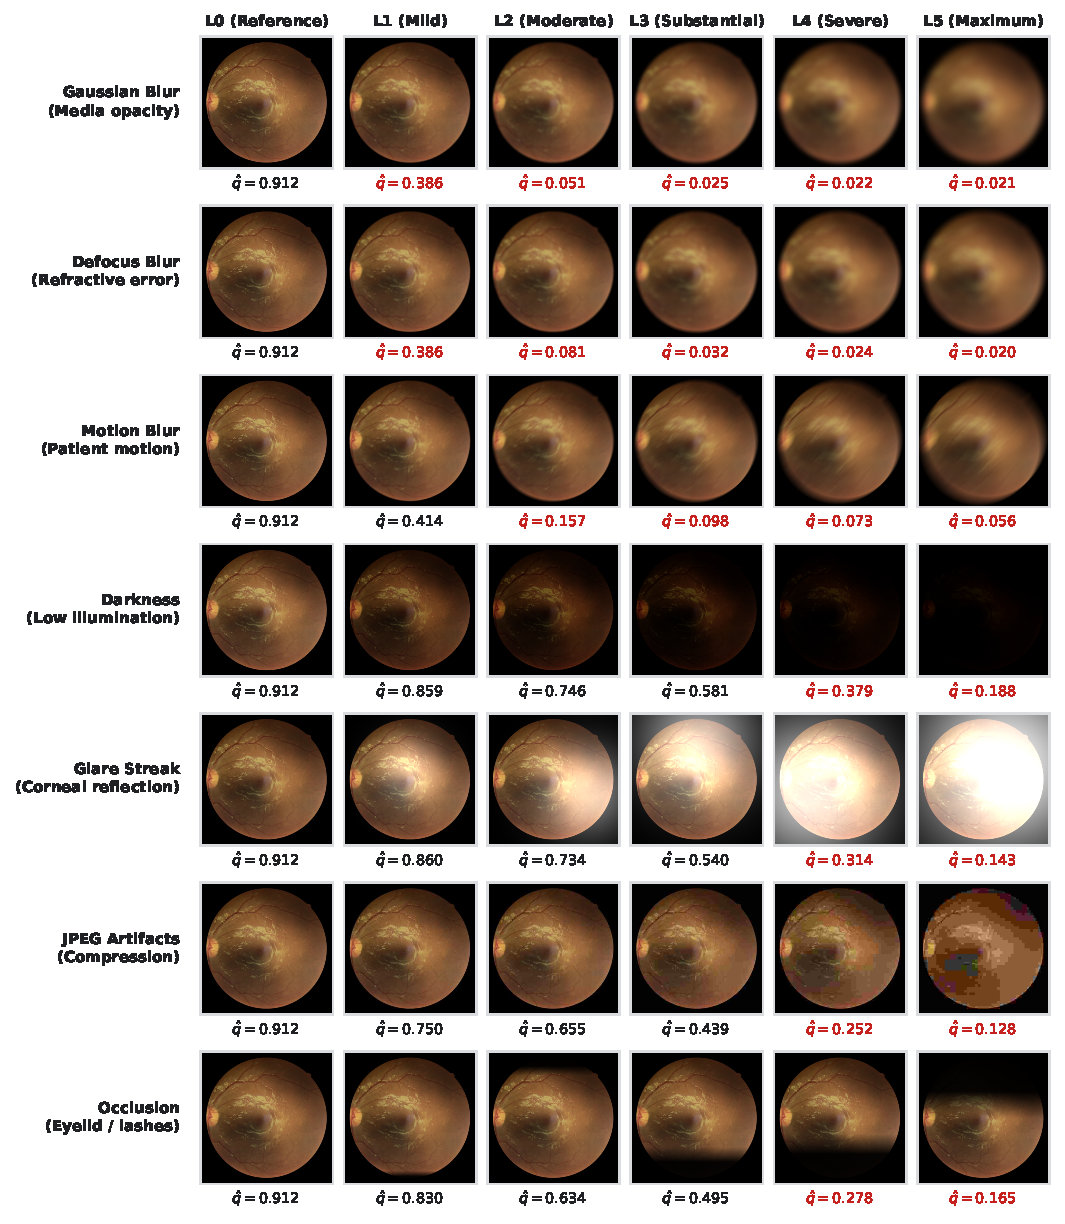
\includegraphics[width=0.9\textwidth]{figures/fig2_degradation_examples.pdf}
\caption{Representative fundus photographs across the seven degradation types at severity levels $L=1$ to $L=5$ alongside the uncorrupted reference photograph ($L=0$). The value under each thumbnail is the mean quality $\bar{q}_2$ estimated by the frozen MobileNetV3 estimator for View~2, averaged over the 200 test pairs and the five evaluation seeds (not the score of the displayed image alone). Values below the illustrative low-quality threshold $q=0.40$, used for display only and not by the model, are shown in red. For Gaussian and defocus blur the mean estimated quality already falls below this threshold at Level~1, although the visual change is subtle. Physical monotonicity metrics and the cohort-wide quality trajectories are given in \ref{app:online_fq_types} (Fig.~\ref{fig:calibration_curves}).}
\label{fig:degrad}
\end{figure*}

\paragraph{Calibration of the degradation parameters} The degradation parameters ($\sigma, r, \ell, \gamma, Q$, occlusion coverage) were calibrated on a validation subset so that the predicted quality $\hat{q}(L)$ of $f_Q$ decreases monotonically towards a target severe-degradation floor of $\approx 0.10$ at Level~5 (Fig.~\ref{fig:calibration_curves}, \ref{app:online_fq_types}). Evaluated over the full test cohort across five seeds and all seven degradation types (Table~\ref{tab:s8_online_fq_types}), the empirical Level-5 mean predicted quality reaches $\bar{q}_2(5) = 0.1032$ (ranging from $0.0202$ for defocus blur to $0.1878$ for darkness), matching the intended severe quality suppression. On the full DeepDRiD test set ($n=400$ images across the $200$ test pairs), the Spearman rank correlation between the estimator's predicted quality $\hat{q}$ and the expert quality score $q^{\text{human}}$ is $\rho = 0.7967$ ($p < 0.001$), indicating substantial rank agreement with expert quality scores on held-out photographs.

\paragraph{Quality scores supplied during the benchmark} In the main benchmark (Sections~\ref{sec:r_degrad} and~\ref{sec:r_safety}), to obtain a reproducible stress test that is decoupled from out-of-distribution errors of $f_Q$ on heavily corrupted images, the quality-conditioned models receive an analytically attenuated score,
\begin{equation}
  q_m(L) = q_m(0) \cdot \left(1 - 0.9 \cdot \frac{L}{5}\right), \qquad L \in \{0,\dots,5\},
  \label{eq:q_attenuation}
\end{equation}
where $q_m(0)$ is the clean-image score: $\hat{q}_m(0) = f_Q(I_m)$ for \qadfnet{} and Q-Weighted GAP in learned mode and $q_m^{\text{human}}(0)$ for the oracle reference (Best-Single and the oracle rows of the ablation). At $L=5$ this gives $q_m(5) = 0.10\,q_m(0) \approx 0.088$ for $q_m(0) \approx 0.88$, close to the empirical floor of $f_Q$ on severely degraded images ($\bar{q}_2(5) = 0.1032$; Section~\ref{sec:r_online_fq}). The rule is the same for all seven types, and Best-Single re-routes according to the attenuated scores. The main benchmark therefore characterises the fusion mechanism \emph{given correct quality information}. The deployable pipeline, in which $f_Q$ is applied to the degraded images, is evaluated in a second protocol (next paragraph; results in Section~\ref{sec:r_online_fq}).

\paragraph{End-to-end protocol with online quality estimation} In the second protocol the analytic rule of Eq.~\eqref{eq:q_attenuation} is dropped. For every degraded pair, $f_Q$ is applied directly to the degraded photograph of each view and the resulting $(\hat q_1, \hat q_2)$ are passed to \qadfnet{} and to Q-Weighted GAP in learned mode. Specifically, $f_Q$ (MobileNetV3) receives the degraded image bilinearly downsampled to $224\times224$, while the dual-view models operate at $448\times448$ using the exact same saved model checkpoints from the main benchmark. Evaluation is conducted under the canonical asymmetric scenario (Scenario~a, View~2 degraded) across the five seeds (42--46), seven degradation types and Levels~0--5. Harm Rate and Help Rate use the same privileged reference view selected from the clean test set predictions, maintaining a consistent ground-truth benchmark for clinical harm auditing. For methods without quality input, their results are identical to the analytic benchmark by construction. Because the degradation strengths were calibrated against this same estimator, this protocol tests whether the outputs of $f_Q$ on these particular corruptions are usable by the fusion module, not whether $f_Q$ generalises to corruptions it was not calibrated on.

\subsection{Statistical analysis}
\label{sec:stats}

Main benchmark comparisons use five seeds (42--46) and ablations three (42--44). Because the two eyes of a patient are not independent, we compute 95\% confidence intervals for QWK and accuracy by a patient-clustered bootstrap \citep{Cameron2015clustboot} with $B=2{,}000$ resamples of whole patients. Pairwise comparisons between \qadfnet{} and each baseline use paired patient-clustered bootstrap tests ($B=2{,}000$) and, where stated, two-sided Wilcoxon signed-rank tests \citep{Wilcoxon1945} over paired test samples. Within a family of baseline comparisons, $p$-values are adjusted by the Holm--Bonferroni procedure \citep{Holm1979} at $\alpha = 0.05$. Table~\ref{tab:main} evaluates pairwise diagnostic differences against \qadfnet{} on the reference seed (seed~42) via paired patient-clustered bootstrap ($B=2{,}000$), adjusted across the $m=9$ baselines of Section~\ref{sec:baselines}. In the degradation benchmark (Table~\ref{tab:degrad_summary}), the family comprises the $m=7$ degradation types for per-type tests and the $m=5$ unconditioned fusion baselines for the overall AUDC test. In the exploratory ablation experiments $p$-values are nominal. Tests across seeds (paired $t$-tests, and Wilcoxon tests over the 35 evaluation runs) describe training variability and not sampling variability of the test set, and are not interchangeable with the patient-clustered bootstrap tests. The end-to-end evaluation with online quality estimation (Section~\ref{sec:r_online_fq}) is descriptive: it reports means and standard deviations over seeds and no significance tests.

%%=================================================================
%%  SECTION 5 --- RESULTS
%%=================================================================
\section{Results}
\label{sec:results}

Section~\ref{sec:r_clean} compares \qadfnet{} with the baselines on clean images as a no-regression check. Section~\ref{sec:r_degrad} reports robustness under the degradation benchmark and Section~\ref{sec:r_safety} clinical safety (Harm Rate, PFR, FDI), including Harm Rate stratified by the natural quality gap between views. Section~\ref{sec:r_online_fq} repeats the degradation benchmark with quality scores estimated online by $f_Q$ from the degraded images. Section~\ref{sec:r_ablation} presents ablations, Section~\ref{sec:r_backbone} backbone variants and computational cost, and Section~\ref{sec:r_prop1} an empirical check of the message bound of Lemma~\ref{lem:1}.

\subsection{Diagnostic performance on clean images}
\label{sec:r_clean}

\qadfnet{} is designed to remain safe under quality asymmetry, not to improve accuracy under ideal acquisition. We therefore first verify that quality conditioning does not degrade performance when both views are good. Table~\ref{tab:main} reports five-seed results on the clean DeepDRiD test set ($n=200$ pairs, 100 patients; the cohort mean predicted quality across all $400$ images is $\hat{q}\approx 0.89$, averaging $0.8688$ for View~1 [macula-centred] and $0.9121$ for View~2 [optic-disc-centred] as evaluated by $f_Q$ on $224\times224$ inputs). \qadfnet{} obtains $\kappa_w = 0.8805 \pm 0.0102$ (95\% CI $[0.8219, 0.9217]$), accuracy $68.70\% \pm 1.86\%$ and macro-AUC $0.9065 \pm 0.0052$.

\begin{table*}[!tb]
\centering
\renewcommand{\arraystretch}{0.7}
\caption{Diagnostic performance on the clean DeepDRiD test set ($n=200$ pairs from 100 patients, five seeds). Values are mean $\pm$ standard deviation over seeds (divisor $N$, $\text{ddof}=0$); 95\% confidence intervals from a patient-clustered bootstrap ($B=2{,}000$). The best value per column is in bold. $p_{\text{Holm}}$ compares each baseline with \qadfnet{} on the reference seed (paired patient-clustered bootstrap with $B=2{,}000$ patient resamples, Holm-adjusted across the family of $m=9$ baselines).}
\label{tab:main}
\footnotesize
\setlength{\tabcolsep}{5.5pt}
\adjustbox{max width=\textwidth}{%
\begin{tabular}{lccccc}
\toprule
Method & QWK (mean $\pm$ std) & QWK [95\% CI] & Accuracy & Macro-AUC & $p_{\text{Holm}}$ \\
\midrule
Single-View V1 (Macula) & 0.8452 $\pm$ 0.0143 & [0.7708, 0.8996] & 0.6670 $\pm$ 0.0236 & 0.8924 $\pm$ 0.0040 & 0.0240 \\
Single-View V2 (Optic Disc) & 0.8376 $\pm$ 0.0137 & [0.7695, 0.8899] & 0.6370 $\pm$ 0.0163 & 0.8761 $\pm$ 0.0105 & $<0.001$ \\
Best-Single (Quality Selector) & 0.8746 $\pm$ 0.0096 & [0.8155, 0.9180] & 0.6890 $\pm$ 0.0252 & 0.8986 $\pm$ 0.0106 & 0.1260 \\
\midrule
Concat & 0.8681 $\pm$ 0.0086 & [0.8071, 0.9127] & 0.6680 $\pm$ 0.0333 & 0.8951 $\pm$ 0.0091 & 0.1350 \\
Max-Pooling & 0.8718 $\pm$ 0.0097 & [0.8121, 0.9149] & 0.6700 $\pm$ 0.0192 & 0.9019 $\pm$ 0.0091 & 0.1260 \\
Standard Cross-Attention & 0.8700 $\pm$ 0.0183 & [0.8076, 0.9139] & 0.6710 $\pm$ 0.0403 & 0.9021 $\pm$ 0.0147 & 0.7220 \\
Average Pooling & 0.8806 $\pm$ 0.0116 & [0.8196, 0.9241] & 0.6940 $\pm$ 0.0285 & 0.9060 $\pm$ 0.0081 & 0.4140 \\
Q-Weighted GAP & 0.8765 $\pm$ 0.0075 & [0.8174, 0.9193] & 0.6830 $\pm$ 0.0175 & 0.9038 $\pm$ 0.0070 & 0.1350 \\
Co-Attention & \textbf{0.8859 $\pm$ 0.0076} & [0.8249, 0.9302] & \textbf{0.7270 $\pm$ 0.0262} & \textbf{0.9125 $\pm$ 0.0026} & 0.7220 \\
\midrule
\qadfnet{} (Proposed) & 0.8805 $\pm$ 0.0102 & [0.8219, 0.9217] & 0.6870 $\pm$ 0.0186 & 0.9065 $\pm$ 0.0052 & --- \\
\bottomrule
\end{tabular}}
\end{table*}

Three observations follow.
\begin{enumerate}
\item \textbf{Dual-view fusion helps modestly.} Every multi-view operator ($\kappa_w = 0.8681$--$0.8859$) exceeds both single-view baselines ($0.8452$ for V1, $0.8376$ for V2), in line with the clinical motivation for combining the two fields. For \qadfnet{} the gain over a single view remains significant after Holm correction ($p_{\text{Holm}}=0.0240$ against V1 and $p_{\text{Holm}}<0.001$ against V2); the other fusion operators were not tested against the single views. The gain is modest in size, however: view selection alone (Best-Single, $\kappa_w=0.8746$; $p_{\text{Holm}}=0.1260$ against \qadfnet{}) already recovers most of it, leaving only about $0.011$ QWK to the best fusion method.
\item \textbf{\qadfnet{} is on par with, not better than, the strongest baselines on clean data.} Its QWK equals that of Average Pooling ($0.8805$ vs.\ $0.8806$), is $0.0040$ above Q-Weighted GAP ($0.8765$) and is $0.0054$ below Co-Attention, which also has the highest accuracy ($72.70\%$ vs.\ $68.70\%$). Apart from the two single-view models (item~1), no baseline differs significantly from \qadfnet{} after correction (smallest adjusted $p=0.1260$, shared by Best-Single and Max-Pooling). With $n=200$ pairs and widely overlapping intervals, this means that we cannot detect a difference, not that the methods are equivalent.
\item \textbf{No detectable clean-image cost of quality conditioning.} At clean quality levels ($\hat q\approx0.87\text{--}0.91$) the logit bias and the Scale-V factor are mild but non-zero, and the sink may still absorb part of the attention mass; the learned parameters ($\beta$, $k_{\text{sink}}$) can compensate. Empirically, QWK stays within the seed-to-seed variability of the unconditioned baselines.
\end{enumerate}
Clean-image performance thus does not separate the fusion strategies; the discriminating evidence for \qadfnet{} lies in robustness and safety under quality asymmetry (Sections~\ref{sec:r_degrad} and~\ref{sec:r_safety}).

\subsection{Degradation robustness}
\label{sec:r_degrad}

We next examine whether the methods differ once one view is corrupted. Table~\ref{tab:degrad_summary} gives the AUDC (Eq.~\eqref{eq:audc}) for the canonical asymmetric scenario (View~2 degraded), and Table~\ref{tab:degrad_scenarios} summarises the three view scenarios. As stated in Section~\ref{sec:degradation}, quality-conditioned models receive the attenuated scores of Eq.~\eqref{eq:q_attenuation}; Section~\ref{sec:r_online_fq} uses online estimates instead.

\begin{table*}[!tb]
\centering
\renewcommand{\arraystretch}{0.7}
\caption{Asymmetric degradation (View~2 degraded, View~1 clean). AUDC over $L\in\{0,\dots,5\}$, mean of five seeds; best value per row in bold. $\Delta_{\text{Co}}$, $\Delta_{\text{Cross}}$: \qadfnet{} minus Co-Attention and Cross-Attention. $p$: two-sided paired patient-clustered bootstrap ($B=2{,}000$) against Co-Attention; $p_{\text{Holm}}$: Holm-adjusted across the seven types (Overall Mean row: across the five unconditioned fusion baselines). $p_{\text{Cross}}$: unadjusted $p$-value against Cross-Attention. Q-W.\ GAP: Q-Weighted GAP (quality-weighted pooling without attention; values from Table~\ref{tab:s1_audc}); evaluated as an architectural ablation control, with no paired bootstrap test reported.}
\label{tab:degrad_summary}
\footnotesize
\setlength{\tabcolsep}{4.2pt}
\adjustbox{max width=\textwidth}{%
\begin{tabular}{lccccccccrccc}
\toprule
Degradation Type & Concat & Average & Max & Cross-Attn & Q-W.\ GAP & Co-Attn & \qadfnet{} [95\% CI] & $\Delta_{\text{Co}}$ & $p$ & $p_{\text{Holm}}$ & $\Delta_{\text{Cross}}$ & $p_{\text{Cross}}$ \\
\midrule
Gaussian Blur    & 0.7959 & 0.8090 & 0.8271 & 0.8367 & 0.8482 & 0.8346 & \textbf{0.8599} [0.8124, 0.8953] & +0.0253 & 0.012 & 0.072 & +0.0232 & 0.019 \\
Defocus Blur     & 0.8237 & 0.8292 & 0.8434 & 0.8443 & 0.8514 & 0.8467 & \textbf{0.8598} [0.8142, 0.8931] & +0.0131 & 0.038 & 0.175 & +0.0155 & 0.032 \\
Motion Blur      & 0.8165 & 0.8143 & 0.8382 & 0.8382 & 0.8506 & 0.8474 & \textbf{0.8609} [0.8150, 0.8974] & +0.0135 & 0.035 & 0.175 & +0.0227 & 0.021 \\
JPEG Compression & 0.8042 & 0.8294 & 0.8347 & 0.8406 & 0.8528 & 0.8369 & \textbf{0.8645} [0.8182, 0.8990] & +0.0276 & 0.008 & 0.056 & +0.0239 & 0.014 \\
Darkness         & 0.8473 & 0.8639 & 0.8644 & 0.8687 & 0.8745 & 0.8732 & \textbf{0.8795} [0.8295, 0.9152] & +0.0063 & 0.124 & 0.372 & +0.0108 & 0.020 \\
Glare            & 0.8254 & 0.8469 & 0.8439 & 0.8594 & 0.8635 & 0.8680 & \textbf{0.8682} [0.8201, 0.9054] & +0.0002 & 0.412 & 0.760 & +0.0088 & 0.048 \\
Occlusion        & 0.8581 & 0.8731 & 0.8676 & 0.8712 & 0.8678 & \textbf{0.8823} & 0.8732 [0.8250, 0.9081] & $-$0.0091 & 0.380 & 0.760 & +0.0020 & 0.382 \\
\midrule
\textbf{Overall Mean} & 0.8245 & 0.8380 & 0.8456 & 0.8513 & 0.8584 & 0.8556 & \textbf{0.8666} [0.8192, 0.9019] & +0.0110 & 0.024 & 0.072 & +0.0153 & 0.038 \\
\bottomrule
\end{tabular}}
\end{table*}

\paragraph{Overall robustness} \qadfnet{} has the highest mean AUDC ($0.8666$), followed by Q-Weighted GAP ($0.8584$), Co-Attention ($0.8556$), Cross-Attention ($0.8513$), Max-Pooling ($0.8456$), Average ($0.8380$) and Concat ($0.8245$). The differences from Average ($+0.0286$, $p_{\text{Holm}}=0.016$) and Concat ($+0.0421$, $p_{\text{Holm}}=0.011$) remain significant after Holm--Bonferroni correction over the five unconditioned fusion baselines (Concat, Average, Max, Cross-Attention, Co-Attention; Q-Weighted GAP is evaluated as an architectural control without paired bootstrap testing). The differences from Co-Attention ($+0.0110$, $p_{\text{Holm}}=0.072$), Cross-Attention ($+0.0153$, $p_{\text{Holm}}=0.076$) and Max-Pooling ($+0.0210$, $p_{\text{Holm}}=0.120$) have the same sign but are not significant. For Max-Pooling the larger mean difference is offset by seed variability: it exceeds \qadfnet{} in two of five seeds (43 and 45), with seed-wise differences $+0.0394$, $-0.0083$, $+0.0410$, $-0.0013$ and $+0.0341$ (paired $t$-test over seeds, $t=1.97$, $df=4$, $p=0.120$).

Expressed as a fraction of its own clean QWK (Table~\ref{tab:main}), the AUDC of \qadfnet{} is $98.4\%$ (mean loss $0.0139$), compared with $97.9\%$ for both Cross-Attention and Q-Weighted GAP, $97.0\%$ for Max-Pooling, $96.6\%$ for Co-Attention, $95.2\%$ for Average and $95.0\%$ for Concat; these descriptive figures were not tested. The difference from Q-Weighted GAP ($+0.0082$) has the same sign, but no paired test was run against this baseline and the difference is smaller than the seed-wise standard deviation of \qadfnet{} ($0.0135$; Table~\ref{tab:degrad_scenarios}).

\paragraph{Effect of quality conditioning} Standard Cross-Attention shares the spatial architecture of \qadfnet{} but uses $q\equiv1$, and is the closest control for quality conditioning (bias, sink, Scale-V and quality-weighted consensus). \qadfnet{} has a higher AUDC than Cross-Attention under all seven degradation types ($+0.0020$ to $+0.0239$). Unadjusted $p$-values are below $0.05$ for six types, but none remains significant after Holm--Bonferroni correction over the seven types (smallest adjusted $p=0.098$, JPEG compression), nor does the overall mean ($p_{\text{Holm}}=0.076$). The consistent direction suggests a benefit of quality conditioning, which is not established for any single type; we treat the per-type tests as exploratory. Q-Weighted GAP is a second control: it carries the quality information but has no spatial attention. Its AUDC is higher than that of Cross-Attention under six of the seven types (overall $+0.0071$; lower only under occlusion, $-0.0034$), so about $46\%$ of the $0.0153$ gap between \qadfnet{} and Cross-Attention is already obtained by quality weighting alone. \qadfnet{} is above Q-Weighted GAP under all seven types ($+0.0047$ to $+0.0117$; overall $+0.0082$; Table~\ref{tab:s1_audc}). We did not test these differences, and the overall gap is below one seed-wise standard deviation, so we cannot say that the part attributable to the sink-augmented spatial attention is reliably different from zero.

\paragraph{Per-type pattern} Relative to Co-Attention, the largest differences occur under JPEG compression ($+0.0276$), Gaussian blur ($+0.0253$), motion blur ($+0.0135$) and defocus blur ($+0.0131$); none is significant after correction over the seven types (smallest adjusted $p=0.056$). Under darkness ($+0.0063$) and glare ($+0.0002$) \qadfnet{} is not distinguishable from Co-Attention, and under occlusion it is lower ($-0.0091$) (all unadjusted $p>0.1$). On these three types Co-Attention exceeds Cross-Attention by $0.0045$--$0.0111$; quality conditioning closes this gap for darkness and glare but only a small part of it for occlusion ($+0.0020$ of $0.0111$). Because the same attenuation rule is applied to all types, these differences cannot be attributed to the quality estimate. One possible, untested explanation is that a single per-image scalar down-weights the whole view even though glare and occlusion leave part of the field intact. Co-Attention operates on pooled vectors without a spatial softmax, so \qadfnet{} differs from it in both spatial interaction and quality conditioning, and we do not attribute the difference to quality conditioning alone.

\paragraph{Severity dependence} At the highest severity ($L=5$), \qadfnet{} reaches $\kappa_w=0.8565\pm0.0150$ ($97.3\%$ of its clean value), compared with $0.8250\pm0.0159$ for Cross-Attention, $0.8158\pm0.0220$ for Co-Attention, $0.7943\pm0.0265$ for Max, $0.7776\pm0.0320$ for Average and $0.7490\pm0.0074$ for Concat. Best-Single, which routes all $200$ pairs to the clean view at this level, reaches $0.8531\pm0.0167$, i.e.\ $0.0034$ below \qadfnet{} and within seed variability. This is consistent with \qadfnet{} approaching clean-view performance at high severity. Best-Single also exceeds Single-View V1 ($0.8452$) although both use the same view, because it is a separately trained checkpoint; differences of about $0.01$ between checkpoints should be interpreted with caution.


\paragraph{Other view scenarios} Table~\ref{tab:degrad_scenarios} gives the mean AUDC for the three scenarios. A single-view model on the intact view retains its clean QWK by construction, whereas one on the degraded view drops to $0.65$--$0.66$; these rows are references only. The more relevant reference is Best-Single, an oracle selector that routes each pair to the view with the higher expert quality grade (on the 200 test pairs View~1 is selected for 80 pairs [$40.0\%$] and View~2 for 120 pairs [$60.0\%$]; $20$ tied pairs go to View~1 because the rule is $q_1^{\text{human}} \ge q_2^{\text{human}}$).

In Scenarios~a and~b, Concat, Average, Max and Cross-Attention have a lower AUDC than Best-Single (by $0.0058$ to $0.0326$), as does Co-Attention in Scenario~a ($-0.0015$); fusion without quality adaptation can thus underperform simply discarding the degraded view. Q-Weighted GAP is above Best-Single in Scenario~a ($+0.0013$, within seed variability) and Scenario~c ($+0.0219$) and below it in Scenario~b ($-0.0067$). \qadfnet{} is above Best-Single in all three scenarios ($+0.0095$, $+0.0043$ and $+0.0231$), but the margins in Scenarios~a and~b are smaller than the seed-to-seed standard deviations and that in Scenario~c is comparable to it, so we regard them as consistent rather than conclusive. In Scenario~b Co-Attention has a slightly higher mean AUDC ($0.8681\pm0.0122$ vs.\ $0.8646\pm0.0107$). \qadfnet{} is above Q-Weighted GAP in all three scenarios ($+0.0082$, $+0.0110$ and $+0.0012$), by less than its own seed-wise standard deviation in Scenarios~a and~c.

In Scenario~c both views are degraded with the same severity, so $q_1/q_2$ is unchanged; the consensus weights of Eq.~\eqref{eq:f_cons} and the routing of Best-Single stay at their clean-data values, and quality conditioning can only attenuate the cross-view messages. The fusion operators lie between $0.689$ and $0.718$ and the differences among Cross-Attention, Q-Weighted GAP, Co-Attention and \qadfnet{} ($\le0.0021$) are within seed variability.

\begin{table*}[!tb]
\centering
\renewcommand{\arraystretch}{0.7}
\caption{Mean AUDC over the seven degradation types for three view scenarios: (a)~View~2 degraded; (b)~View~1 degraded; (c)~both degraded. Mean $\pm$ standard deviation over five seeds; best value per column in bold. Best-Single is a separately trained checkpoint, not the Single-View rows.}
\label{tab:degrad_scenarios}
\footnotesize
\begin{tabular}{lccc}
\toprule
Method & (a) V2 degraded & (b) V1 degraded & (c) Both degraded \\
\midrule
Single-View V1 (Macula)       & 0.8452 $\pm$ 0.0143 & 0.6533 $\pm$ 0.0251 & 0.6533 $\pm$ 0.0251 \\
Single-View V2 (Optic Disc)   & 0.6639 $\pm$ 0.0379 & 0.8376 $\pm$ 0.0137 & 0.6639 $\pm$ 0.0379 \\
Best-Single (Quality Selector)& 0.8571 $\pm$ 0.0149 & 0.8603 $\pm$ 0.0076 & 0.6951 $\pm$ 0.0236 \\
Concat                        & 0.8245 $\pm$ 0.0062 & 0.8286 $\pm$ 0.0100 & 0.7059 $\pm$ 0.0138 \\
Average                       & 0.8380 $\pm$ 0.0176 & 0.8369 $\pm$ 0.0146 & 0.6889 $\pm$ 0.0388 \\
Max                           & 0.8456 $\pm$ 0.0161 & 0.8399 $\pm$ 0.0156 & 0.7117 $\pm$ 0.0322 \\
Cross-Attention               & 0.8513 $\pm$ 0.0123 & 0.8474 $\pm$ 0.0137 & 0.7169 $\pm$ 0.0314 \\
Q-Weighted GAP                & 0.8584 $\pm$ 0.0052 & 0.8536 $\pm$ 0.0079 & 0.7170 $\pm$ 0.0130 \\
Co-Attention                  & 0.8556 $\pm$ 0.0128 & \textbf{0.8681 $\pm$ 0.0122} & 0.7161 $\pm$ 0.0358 \\
\midrule
\textbf{\qadfnet{} (Ours)}    & \textbf{0.8666 $\pm$ 0.0135} & 0.8646 $\pm$ 0.0107 & \textbf{0.7182 $\pm$ 0.0161} \\
\bottomrule
\end{tabular}
\end{table*}

\begin{figure*}[!tb]
\centering
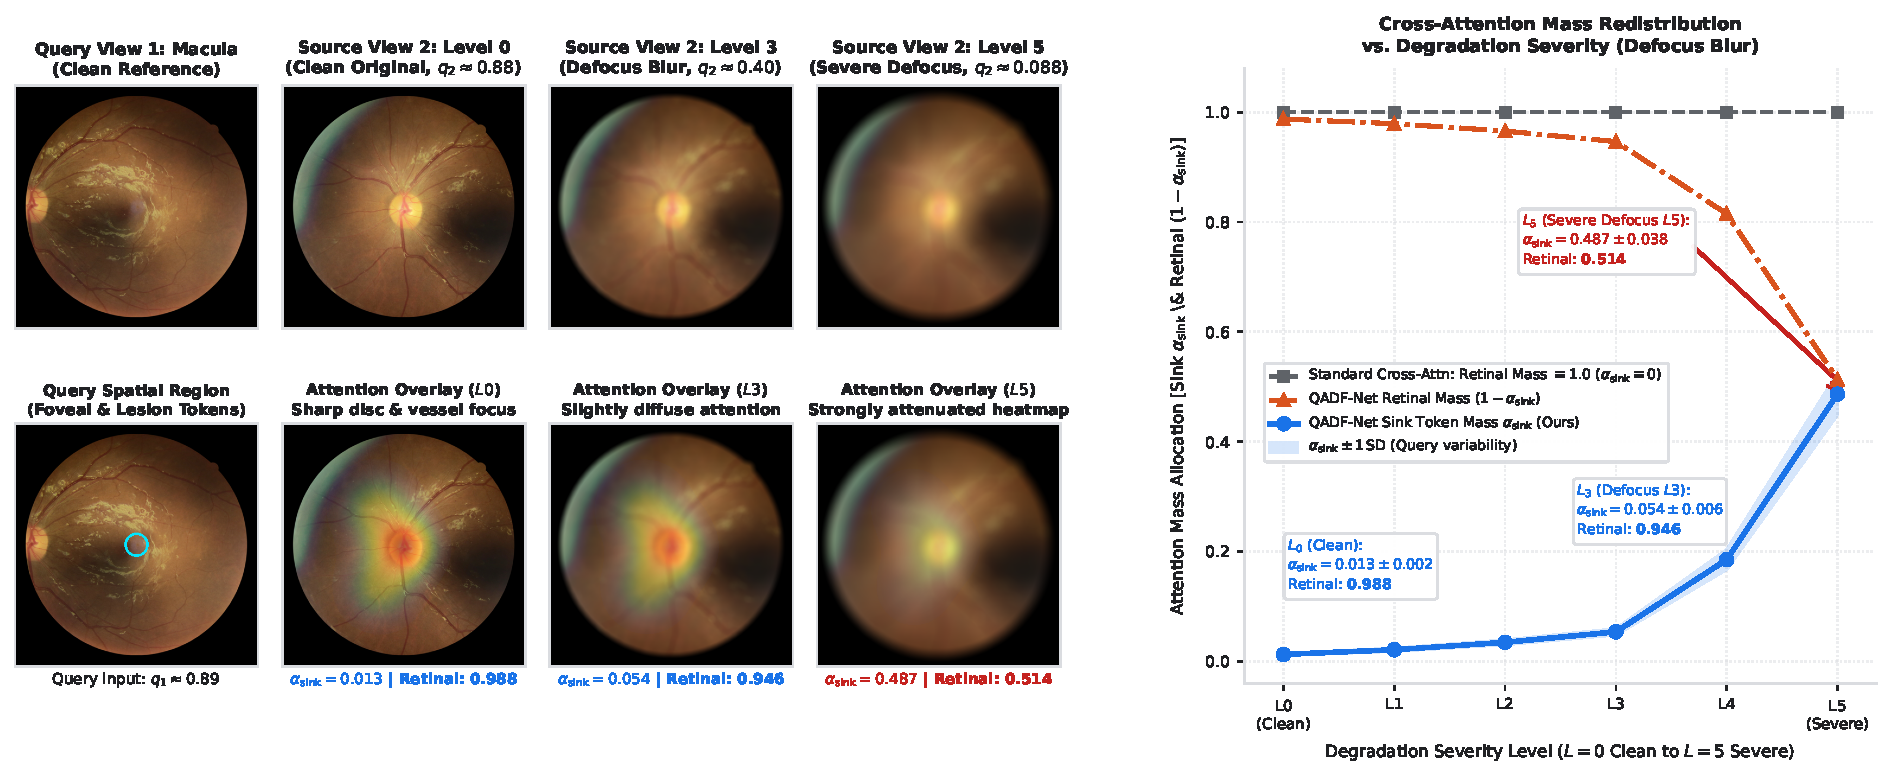
\includegraphics[width=0.8\textwidth]{figures/fig4_attention_maps.pdf}
\caption{Cross-attention maps and attention-mass allocation for one representative test pair under increasing defocus blur. Top row: query View~1 (macula-centred, clean, $q_1 \approx 0.89$) and source View~2 (optic-disc-centred) at Level~0 ($q_2 \approx 0.88$), Level~3 ($q_2 \approx 0.40$) and Level~5 ($q_2 \approx 0.088$); these $q_2$ values are the analytically attenuated scores of Eq.~\eqref{eq:q_attenuation} used in the main benchmark. Bottom row: query region (foveal and lesion tokens) and the corresponding cross-attention maps overlaid on the source photographs; attention is concentrated on the optic disc and vascular arcades at Level~0, more diffuse at Level~3 and strongly attenuated at Level~5. Right panel: sink mass $\alpha_{\text{sink}}$ (0.0125 at Level~0, 0.0536 at Level~3 and 0.4865 at Level~5; mean over queries, with a $\pm1$ SD band) and residual mass $1-\alpha_{\text{sink}}$ on genuine tokens, compared with standard cross-attention, in which all mass lies on the corrupted tokens ($\alpha_{\text{sink}} \equiv 0$). Values printed inside the panels are rounded to three decimals.}
\label{fig:attn_maps}
\end{figure*}

\subsection{Clinical safety: Harm Rate, prediction stability and feature drift}
\label{sec:r_safety}

Aggregate agreement can hide pair-level failures, so we also ask whether fusion makes individual predictions worse than the single view it could have relied on, and how stable predictions are when one view degrades. Harm Rate and Help Rate (Eqs.~\eqref{eq:harm_rate} and~\eqref{eq:help_rate}) are computed against $\hat{y}_{\text{best\_view}}$, the prediction of the view with the higher expert quality score on the clean test pairs, held fixed across all severity levels as an invariant privileged reference, like that of Best-Single. All rates are computed over the $200$ test pairs. We compare \qadfnet{} with the five unconditioned fusion baselines; Harm Rate is not computed for Best-Single, a single-view model, which enters only the flip-rate comparison. Q-Weighted GAP is omitted from Table~\ref{tab:harm_flip} because its safety metrics were not tabulated across all severity levels under the analytic protocol and no paired bootstrap tests were run for it; its safety profile is characterised instead through the three-seed ablation protocol in Table~\ref{tab:ablation} ($\text{HR}_{L5} = 15.68\%$, $\text{PFR}_{L5} = 24.20\%$, against $14.52\%$ and $21.78\%$ for the default configuration) and across full severity levels under online quality estimation in Table~\ref{tab:online_fq_benchmark} ($15.82\%$ and $24.60\%$, against $14.63\%$ and $23.40\%$ for \qadfnet{}).

\paragraph{Safety under controlled degradation} Table~\ref{tab:harm_flip} reports Harm Rate, PFR and FDI for severity levels $0$--$5$ in the canonical asymmetric scenario (View~2 degraded). Level~0 is the five-seed mean; Levels~1--5 are means over all five seeds and seven degradation types ($35$ evaluations per level).

\begin{table*}[!tb]
\centering
\caption{Safety metrics versus degradation severity (Level~0 = clean) for the asymmetric scenario (View~2 degraded, View~1 clean). Level~0 reports the five-seed mean; Levels~1--5 report the mean over $35$ evaluations ($5$ seeds $\times$ $7$ types). ``Mean'' is the unweighted mean over L1--L5; $\Delta$ is the change in Harm Rate from Level~0 to Level~5 in percentage points (pp). PFR is zero at Level~0 by definition. FDI is normalised by the clean consensus vector of each method, so values are comparable across methods in relative terms only. The best value per column within each metric block is in bold.}
\label{tab:harm_flip}
\footnotesize
\renewcommand{\arraystretch}{0.7}
\setlength{\tabcolsep}{4.5pt}
\adjustbox{max width=\textwidth}{%
\begin{tabular}{lcccccccc}
\toprule
Method & L0 (clean) & L1 & L2 & L3 & L4 & L5 & Mean L1--L5 & $\Delta$ (pp) \\
\midrule
\multicolumn{9}{l}{\textbf{Harm Rate (\%)}} \\
\quad Concat          & 12.50 & 12.99 & 15.57 & 18.29 & 24.24 & 28.79 & 19.98 & $+16.29$ \\
\quad Average         & 11.60 & 12.66 & 15.96 & 19.41 & 23.51 & 27.23 & 19.75 & $+15.63$ \\
\quad Max-Pooling     & 13.00 & 12.71 & 14.36 & 16.70 & 19.96 & 23.74 & 17.49 & $+10.74$ \\
\quad Cross-Attention & 13.00 & 13.41 & 15.64 & 17.39 & 18.69 & 18.79 & 16.78 & $+5.79$ \\
\quad Co-Attention    & \textbf{9.00} & \textbf{9.84} & \textbf{12.14} & 15.51 & 19.56 & 21.50 & 15.71 & $+12.50$ \\
\quad \qadfnet{} (Ours) & 12.30 & 12.59 & 13.10 & \textbf{13.96} & \textbf{14.29} & \textbf{14.49} & \textbf{13.69} & $\mathbf{+2.19}$ \\
\midrule
\multicolumn{9}{l}{\textbf{Prediction Flip Rate (PFR, \%)}} \\
\quad Concat          & 0.00 & 12.14 & 19.66 & 25.76 & 34.57 & 41.61 & 26.75 & --- \\
\quad Average         & 0.00 & 11.76 & 19.09 & 26.69 & 33.47 & 39.19 & 26.04 & --- \\
\quad Max-Pooling     & 0.00 & 12.09 & 19.09 & 25.24 & 30.46 & 35.79 & 24.53 & --- \\
\quad Cross-Attention & 0.00 & 12.13 & 19.04 & 23.29 & 26.79 & 28.67 & 21.98 & --- \\
\quad Co-Attention    & 0.00 & \textbf{9.34} & \textbf{16.07} & 21.80 & 27.46 & 30.50 & 21.03 & --- \\
\quad Best-Single     & 0.00 & 20.26 & 23.99 & 24.03 & 23.90 & 23.90 & 23.22 & --- \\
\quad \qadfnet{} (Ours) & 0.00 & 13.97 & 17.94 & \textbf{20.89} & \textbf{22.20} & \textbf{21.84} & \textbf{19.37} & --- \\
\midrule
\multicolumn{9}{l}{\textbf{Feature Drift Index (FDI)}} \\
\quad Concat          & 0.0000 & 0.2528 & 0.4012 & 0.5751 & 0.7728 & 0.9663 & 0.5936 & --- \\
\quad Average         & 0.0000 & \textbf{0.2301} & \textbf{0.3574} & 0.4943 & 0.6453 & 0.7924 & 0.5039 & --- \\
\quad Max-Pooling     & 0.0000 & 0.2862 & 0.4279 & 0.5753 & 0.7395 & 0.8988 & 0.5855 & --- \\
\quad Cross-Attention & 0.0000 & 0.2635 & 0.3777 & 0.4641 & 0.5471 & 0.6141 & 0.4533 & --- \\
\quad Co-Attention    & 0.0000 & 0.2572 & 0.4220 & 0.5976 & 0.7846 & 0.9531 & 0.6029 & --- \\
\quad \qadfnet{} (Ours) & 0.0000 & 0.2747 & 0.3707 & \textbf{0.4256} & \textbf{0.4686} & \textbf{0.4793} & \textbf{0.4038} & --- \\
\midrule
\multicolumn{9}{l}{\textbf{QWK ($\kappa_w$) of \qadfnet{}}} \\
\quad \qadfnet{} ($\kappa_w$) & 0.8805 & 0.8755 & 0.8682 & 0.8621 & 0.8584 & 0.8565 & 0.8641 & --- \\
\bottomrule
\end{tabular}}
\end{table*}

\begin{figure*}[!tb]
\centering
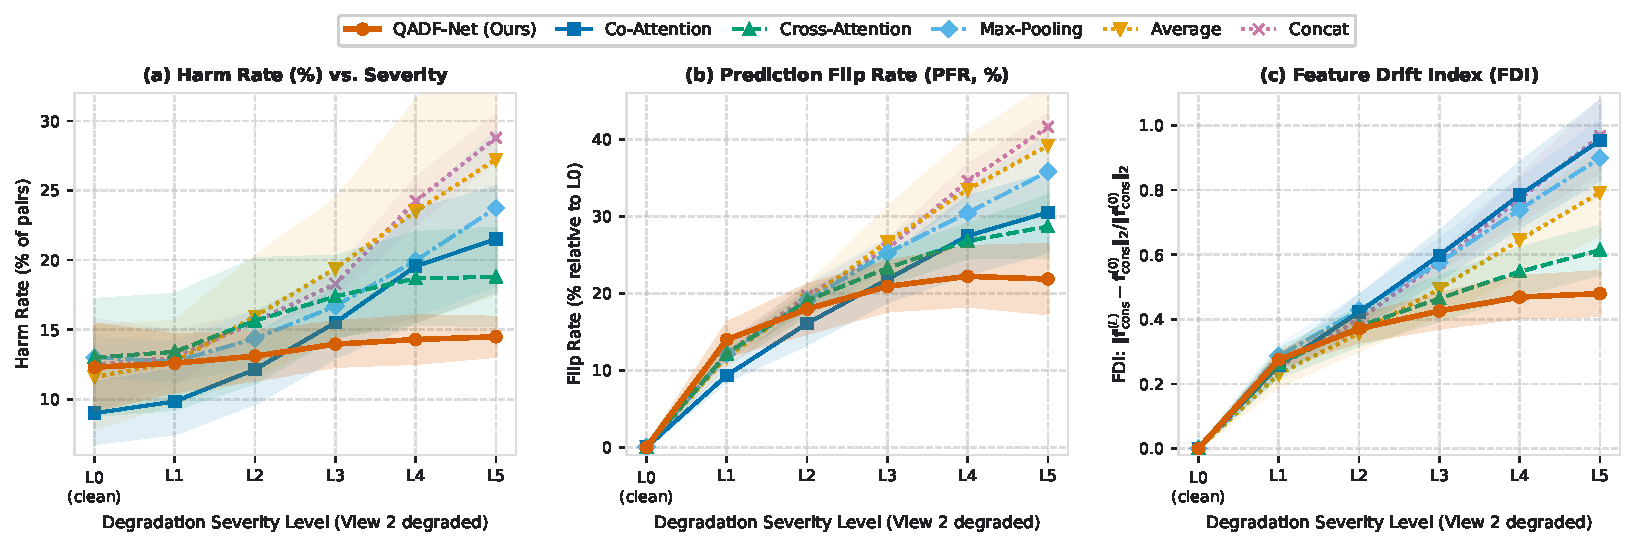
\includegraphics[width=\textwidth]{figures/fig5_safety_profiles.pdf}
\caption{Clinical safety and representation stability metrics across degradation severity levels ($L0 \to L5$, View~2 degraded) for the six fusion methods: (a)~Harm Rate (Eq.~\eqref{eq:harm_rate}), (b)~Prediction Flip Rate (PFR, Eq.~\eqref{eq:pfr}), and (c)~Feature Drift Index (FDI, Eq.~\eqref{eq:fdi}). Points denote the five-seed mean averaged over seven degradation types; shaded bands denote $95\%$ confidence intervals derived from a $t$-distribution on four degrees of freedom ($n=5$ seeds). From Level~3 onwards \qadfnet{} has the lowest Harm Rate, flip rate and feature drift of the six methods; its Harm Rate grows by $2.19$~pp from $L0$ to $L5$.}
\label{fig:safety_profiles}
\end{figure*}

\paragraph{Harm Rate} Harm Rate is higher at Level~5 than at Level~0 for every fusion method (Table~\ref{tab:harm_flip} and Fig.~\ref{fig:safety_profiles}a), but the increase differs strongly: $+16.29$ percentage points (pp) for Concat (to $28.79\%$), $+15.63$~pp for Average ($27.23\%$), $+12.50$~pp for Co-Attention ($21.50\%$), $+10.74$~pp for Max-Pooling ($23.74\%$) and $+5.79$~pp for Cross-Attention ($18.79\%$), against $+2.19$~pp for \qadfnet{}, whose Level-5 value is $14.49\% \pm 1.13\%$ (mean $\pm$ standard deviation over five seeds, $\text{ddof}=0$; $95\%$ CI $[12.91\%, 16.06\%]$ from the sample standard deviation $s=1.27\%$ with a $t$-distribution on four degrees of freedom). The Level-0 values ($9.00\%$--$13.00\%$) reflect ordinary disagreement between independently trained fused and single-view models and act as a floor, so the growth relative to Level~0 is the more informative quantity.

At Level~5, paired two-sided $t$-tests over the five seeds give a significantly lower Harm Rate for \qadfnet{} than for Concat ($-14.30$~pp, raw $p<0.001$, $p_{\text{Holm}}<0.001$), Co-Attention ($-7.01$~pp, raw $p=0.004$, $p_{\text{Holm}}=0.016$), Max-Pooling ($-9.25$~pp, raw $p=0.006$, $p_{\text{Holm}}=0.019$), Cross-Attention ($-4.30$~pp, raw $p=0.016$, $p_{\text{Holm}}=0.032$) and Average ($-12.74$~pp, raw $p=0.018$, $p_{\text{Holm}}=0.032$). With five seeds these tests have limited power and describe training variability, not sampling variability of the test set. Averaged over L1--L5, \qadfnet{} has the lowest Harm Rate ($13.69\%$, against $15.71\%$ to $19.98\%$ for the baselines).

\paragraph{Prediction stability} The flip rate shows the same ordering at high severity (Fig.~\ref{fig:safety_profiles}b). At Level~5, $41.61\%$ of Concat predictions, $39.19\%$ of Average, $35.79\%$ of Max-Pooling, $30.50\%$ of Co-Attention and $28.67\%$ of Cross-Attention predictions change grade relative to the clean classification, against $21.84\% \pm 3.70\%$ for \qadfnet{} ($95\%$ CI $[20.61\%, 23.07\%]$ across the $35$ evaluation runs). These $35$ runs share the same seeds and test pairs and are not independent, so the interval and the tests below are nominal and best read as descriptive. Paired comparisons across the $35$ evaluations give a lower Level-5 flip rate for \qadfnet{} than for Cross-Attention ($-6.83$~pp, $95\%$ CI $[-9.31, -4.33]$, Wilcoxon $p=4.38\times10^{-5}$), Co-Attention ($-8.66$~pp, $[-11.96, -5.39]$, $p=5.03\times10^{-5}$), Max-Pooling ($-13.94$~pp, $[-17.03, -10.81]$, $p<10^{-6}$), Average ($-17.34$~pp, $[-21.54, -13.39]$, $p<10^{-6}$) and Concat ($-19.77$~pp, $[-23.70, -15.97]$, $p<10^{-6}$); all five Holm-adjusted $p$-values are below $0.001$.

\qadfnet{} also has a lower flip rate than Best-Single ($21.84\%$ vs.\ $23.90\%$), but the two are not directly comparable, because most flips of Best-Single are the intended consequence of re-routing to the intact view. Its flip rate jumps to $20.26\%$ at Level~1, which tracks view routing: as $q_2$ attenuates, $56$ pairs ($28.0\%$ of the cohort) switch their selected view from View~2 to View~1. It plateaus near $23.90\%$ from Level~2 onwards, once routing to View~1 reaches $95.5\%$ ($191/200$ pairs) and finally $100\%$ at Levels~4--5.

\paragraph{Scope of the advantage} The advantage depends on severity. \qadfnet{} has the lowest Harm Rate and PFR from Level~3 onwards, but not at low severity: Co-Attention has the lowest Harm Rate at Levels~0--2 ($9.00\%$, $9.84\%$, $12.14\%$ vs.\ $12.30\%$, $12.59\%$, $13.10\%$) and the lowest PFR at Levels~1 and~2, and at Level~1 \qadfnet{} has a higher PFR ($13.97\%$) than all fusion baselines. Quality conditioning therefore does not lower Harm Rate or flip rate on clean or mildly degraded pairs; it limits their growth as one view fails. Relative to Cross-Attention, the closest architectural control, \qadfnet{} has a lower Harm Rate at every level, although the gaps at Levels~0 and~1 are below $1$~pp and were not tested. Co-Attention operates on pooled vectors without spatial attention, so its advantage at low severity should not be read as a property of quality conditioning.

\paragraph{Natural quality gap} Table~\ref{tab:gap_strata} asks whether diagnostic stability is preserved without synthetic degradation, by stratifying the unperturbed test pairs by the natural quality difference $|q_1 - q_2|$ in two ways: (i)~by $q^{\text{human}}$, in approximate tertiles of the expert gap ($|q_1 - q_2| \le 2/30 \approx 0.067$, $n=75$, comprising $20$ exactly tied pairs and $55$ pairs with a gap of at most $2/30$; $0.067 < |q_1 - q_2| \le 0.200$, $n=74$; $>0.200$, $n=51$; the discreteness of the expert score prevents equal-sized strata) and (ii)~by $\hat{q}$, in tertiles of the gap of the MobileNetV3 estimator ($\le 0.083$, $n=67$; $0.083$--$0.167$, $n=66$; $>0.167$, $n=67$). In both stratifications $\hat{y}_{\text{best\_view}}$ is selected with $q^{\text{human}}$; only the grouping differs.

\begin{table*}[!tb]
\centering
\renewcommand{\arraystretch}{0.7}
\caption{Harm Rate, Help Rate, QWK and baseline Harm Rates on the unperturbed test set ($200$ pairs), stratified by the natural quality gap $|q_1-q_2|$ (approximate tertiles). Fusion Gain is the QWK of \qadfnet{} minus that of Best-Single. Values denote the five-seed mean, yielding a pooled Harm Rate of $12.30\%$ and a pooled Help Rate of $16.90\%$, in exact agreement with the unperturbed baseline in Table~\ref{tab:harm_flip} and Table~\ref{tab:online_fq_benchmark}. The last column gives the minimum and maximum Harm Rate of the five fusion baselines in the same stratum.}
\label{tab:gap_strata}
\footnotesize
\setlength{\tabcolsep}{4.5pt}
\adjustbox{max width=\textwidth}{%
\begin{tabular}{llccccccc}
\toprule
Quality metric & Gap stratum & Pairs & QWK \qadfnet{} & QWK Best-Single & Fusion Gain & Harm Rate & Help Rate & Baseline Harm Range \\
\midrule
\multirow{3}{*}{$q^{\text{human}}$}
  & Low ($\le 0.067$)            & 75 & 0.8982 & 0.8650 & $+0.0332$ & 11.73\% & 16.53\% & 8.80\%--17.33\% \\
  & Medium ($0.067$--$0.200$)     & 74 & 0.9095 & 0.9055 & $+0.0040$ & 13.24\% & 17.30\% & 9.46\%--15.14\% \\
  & High ($> 0.200$)             & 51 & 0.8122 & 0.8140 & $-0.0018$ & 11.76\% & 16.86\% & 7.84\%--13.73\% \\
\midrule
\multirow{3}{*}{$\hat{q}$}
  & Low ($\le 0.083$)            & 67 & 0.9180 & 0.8860 & $+0.0320$ & 11.94\% & 17.31\% & 6.57\%--13.43\% \\
  & Medium ($0.083$--$0.167$)     & 66 & 0.8080 & 0.7780 & $+0.0300$ & 12.12\% & 16.36\% & 9.09\%--15.45\% \\
  & High ($> 0.167$)             & 67 & 0.9136 & 0.8978 & $+0.0158$ & 12.84\% & 17.01\% & 10.45\%--14.93\% \\
\bottomrule
\end{tabular}}
\end{table*}

We make three observations. First, Help Rate exceeds Harm Rate in every stratum by a factor of $1.3$ to $1.5$ ($16.36\%$--$17.31\%$ vs.\ $11.73\%$--$13.24\%$), so on natural pairs fusion with \qadfnet{} reduces the error relative to $\hat{y}_{\text{best\_view}}$ more often than it increases it ($33.8$ against $24.6$ pairs of $200$, i.e.\ $16.90\%$ vs.\ $12.30\%$). Second, Harm Rate shows no consistent trend with the natural gap: under $q^{\text{human}}$ it is $11.73\%$, $13.24\%$ and $11.76\%$ from the Low to the High tier, and under $\hat{q}$ it rises slightly from $11.94\%$ to $12.12\%$ and $12.84\%$; the differences correspond to one to two pairs per stratum. The Harm Rate of \qadfnet{} lies inside the range of the baselines' Harm Rates in all six strata, so on natural pairs the table shows neither an advantage nor a disadvantage in Harm Rate. This is expected: natural pairs are mostly of good quality ($\bar{q} \approx 0.88$), and even in the High tier the mean pair quality remains high ($\bar{q}_{\text{pair}} \ge 0.70$; clearer view $\bar{q}_{\text{max}} \approx 0.87$, lower-quality view $\bar{q}_{\text{min}} \approx 0.55$--$0.59$). Across all $400$ test photographs only $1$ ($0.25\%$) has $q^{\text{human}} < 0.20$ (specifically $q = 0.067$) and only $2$ ($0.50\%$) have $\hat{q} < 0.20$. The natural test set therefore contains virtually no severely degraded views, which is why pronounced differences between fusion operators appear primarily under controlled degradation. Third, the QWK gain over Best-Single is positive in five of six strata (largest $+0.0332$) and shrinks as the gap grows under both definitions; these QWKs rest on $51$--$75$ pairs across five seeds and the gains are small ($+0.0059$ overall, not significant; Table~\ref{tab:main}), so we regard them as descriptive.

\paragraph{Representation drift} Table~\ref{tab:harm_flip} and Fig.~\ref{fig:safety_profiles}c report the FDI of the six fusion operators. Between Levels~4 and~5 the FDI of the baselines still rises, by $+0.067$ (Cross-Attention) to $+0.194$ (Concat), reaching $0.6141$ (Cross-Attention), $0.7924$ (Average), $0.8988$ (Max-Pooling), $0.9531$ (Co-Attention) and $0.9663$ (Concat) at Level~5; a value close to $1$ means that the consensus vector has moved by about its own norm. For \qadfnet{} the FDI reaches $0.4793$ at Level~5 with shrinking increments ($+0.0960$, $+0.0549$, $+0.0430$ and $+0.0107$ for Levels~2 to~5); it is the lowest of the six from Level~3 onwards and on average over L1--L5 ($0.4038$). At low severity this does not hold: at Level~1 only Max-Pooling has a higher FDI than \qadfnet{} ($0.2747$), and at Levels~1 and~2 Average has the lowest FDI ($0.2301$ and $0.3574$ vs.\ $0.2747$ and $0.3707$). Three caveats apply. First, FDI measures departure from the clean fused representation, which includes the intended down-weighting of View~2, so it is not a direct measure of contamination. Second, a displacement of about $0.5$ is not small, and it already reaches $0.27$ at Level~1. Third, FDI does not separate the components of \qadfnet{} and does not test the message bound of Lemma~\ref{lem:1}, which concerns the cross-view message only (Section~\ref{sec:r_prop1}); the flattening is consistent with bounded-message behaviour but does not confirm it.

\paragraph{Redistribution of spatial attention} Fig.~\ref{fig:attn_maps} shows cross-attention maps from the macula view (queries) to the optic-disc view (keys and values) for a representative test pair under increasing defocus blur. On the clean pair ($q_2 \approx 0.88$) the sink absorbs only $\alpha_{\text{sink}} = 0.0125 \pm 0.0020$ of the attention mass across spatial queries (cohort clean baseline $0.0118 \pm 0.0025$), so over $98.7\%$ of the mass stays on genuine retinal tokens. As $q_2$ decreases, the penalty $|\beta|\log q_2$ on genuine tokens moves mass progressively to $\tau_{\text{sink}}$: $\alpha_{\text{sink}}$ rises to $0.0536 \pm 0.0058$ at Level~3 ($q_2 \approx 0.40$) and to $0.4865 \pm 0.0380$ at Level~5 ($q_2 \approx 0.088$), with some heavily degraded queries routing over $70\%$ of their mass to the sink. In the notation of Section~\ref{sec:prop1}, the weight on genuine token $j$ is $\alpha_{ij}=g_i(q_2)\,p_{ij}$, so the sink rescales the cross-view update by a query-dependent factor without altering the relative distribution over genuine tokens, and the mass it absorbs carries a zero value vector.

For this pair at Level~5, the residual mass on genuine tokens, averaged over queries, is $1-\alpha_{i,\text{sink}} \approx 0.5135$, which is then multiplied by the Scale-V factor $q_2 \approx 0.088$; the compound factor $q_2\, g_i(q_2)$ is therefore about $0.045$, i.e.\ the cross-view message retains on average about $4.5\%$ of its unmodulated magnitude. This is an average over the queries of a single pair, not a cohort statistic or a per-query guarantee. The separate contributions of the sink and of Scale-V are examined in Section~\ref{sec:r_ablation}.

\paragraph{Qualitative case studies}
Fig.~\ref{fig:qualitative_cases} shows two dual-view cases from the test cohort under controlled degradation: one in which \qadfnet{} corrects the error made by other operators, and one in which it fails. The cases are illustrative and support no quantitative claim.
Both cases were selected by the authors, one to illustrate the proposed mechanism and one to illustrate a limitation, and were not drawn at random; they therefore say nothing about how often either outcome occurs. Neither quality score was obtained by applying $f_Q$ to the degraded photograph shown. In Case~1, $\hat{q}_2 = 0.12$ is the analytically attenuated score of Eq.~\eqref{eq:q_attenuation} used in the main benchmark, i.e.\ $0.28\,q_2(0)$ at $L=4$ with $q_2(0) \approx 0.43$ for this pair. It is therefore not comparable with the cohort mean $\bar{q}_2 = 0.024$ for defocus blur at $L=4$ in Fig.~\ref{fig:degrad}, which is the output of $f_Q$ applied to the degraded photographs (averaged over the 200 test pairs and five seeds) and, for this degradation type, lies far below the type-independent analytic rule. In Case~2, $\hat{q}_2 = 0.54$ is the cohort-mean estimate of $f_Q$ for glare at $L=3$ (Fig.~\ref{fig:degrad}), assigned to this pair rather than computed on its own degraded photograph.

\emph{Case~1: success under severe defocus blur} (Fig.~\ref{fig:qualitative_cases}a). Patient~353 (left eye; ground truth Grade~3, severe NPDR) has a macula view of good estimated quality ($\hat{q}_1 = 0.89$) and an optic-disc view degraded by defocus blur ($L=4$, $\hat{q}_2 = 0.12$). Concat and Average both predict Grade~2, and Cross-Attention predicts Grade~1 (an error of two grades), whereas \qadfnet{} predicts the correct Grade~3. For this pair, $68.4\%$ of the cross-attention mass is routed to the sink token, which carries a zero value vector, so little information from the degraded disc view enters the macula representation. This is consistent with the proposed mechanism but does not prove it.

\emph{Case~2: failure under a localised glare streak} (Fig.~\ref{fig:qualitative_cases}b). Patient~383 (left eye; ground truth Grade~2, moderate NPDR) has a glare streak across the upper vascular arcade of View~2. The quality score supplied for this view is the cohort-mean $f_Q$ estimate for glare at $L=3$ ($\hat{q}_2 = 0.54$), which remains comparatively high, presumably because the glare covers only part of the field; we did not test this. With this score the sink absorbs only $18.2\%$ of the attention mass. Concat, Average, Cross-Attention and \qadfnet{} all predict Grade~3 (an error of one grade). The attention maps of Cross-Attention and \qadfnet{} both place weight on the high-contrast glare boundary, which may have been mistaken for exudative pathology; we did not test this explanation. The case illustrates a limitation of scalar quality conditioning (Limitation~(iv)): when degradation is spatially non-uniform, a single scalar cannot suppress corrupted sub-regions without also attenuating intact diagnostic ones, which motivates spatial quality maps.

\begin{figure*}[!tb]
\centering
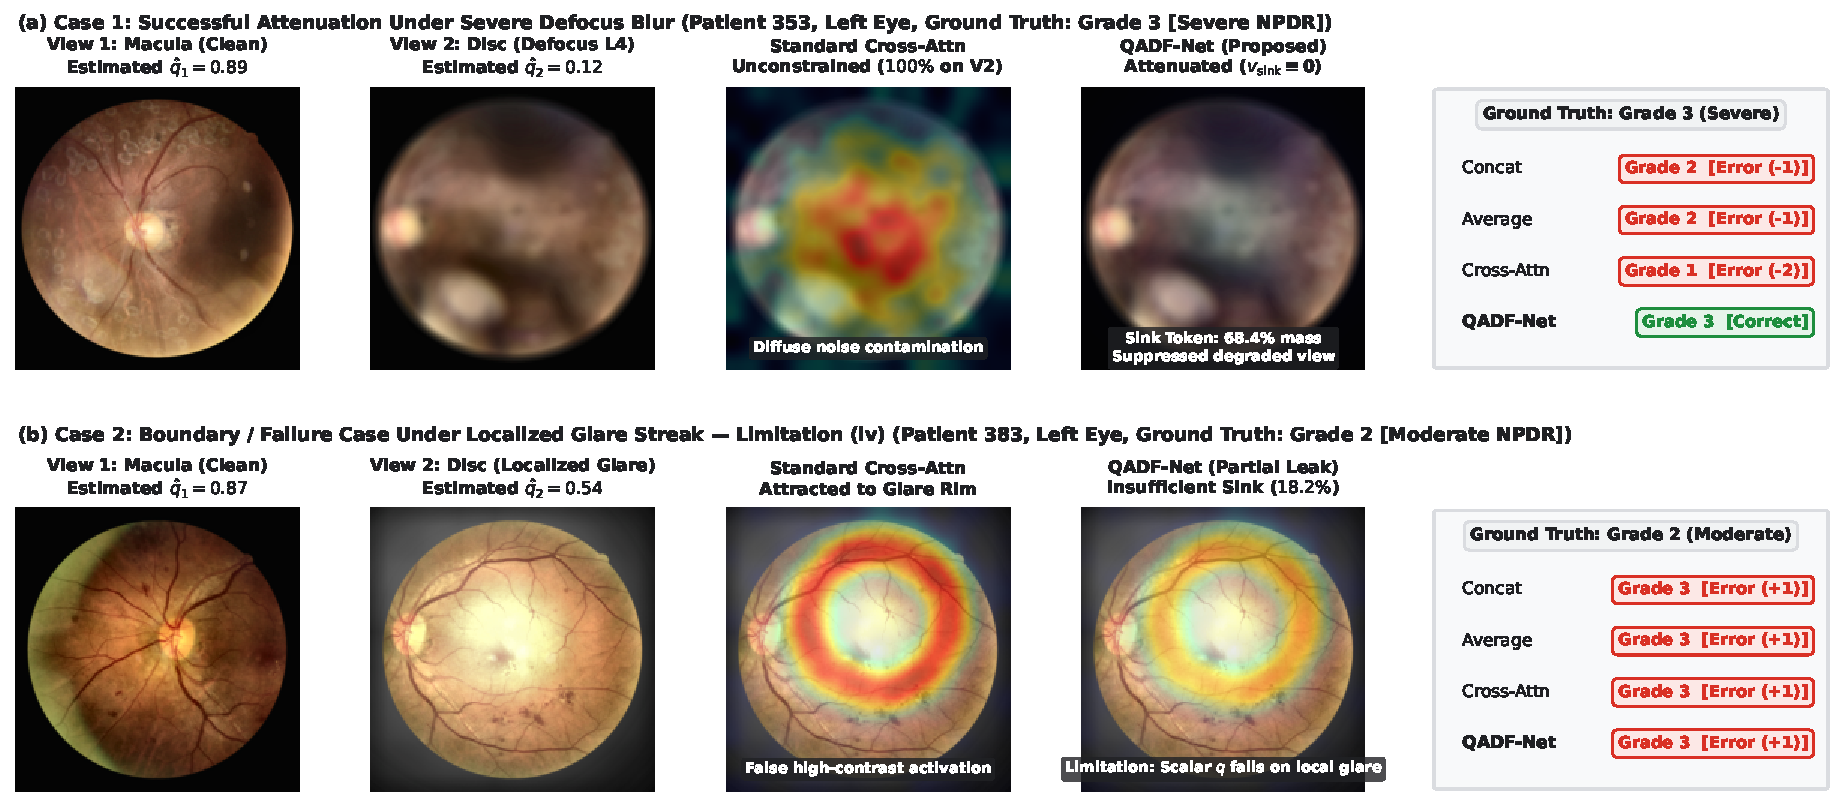
\includegraphics[width=0.9\textwidth]{figures/fig6_qualitative_cases.pdf}
\caption{Illustrative case studies on asymmetric dual-view pairs from the DeepDRiD test cohort under controlled degradation. (a)~Success under severe defocus blur: patient~353 (left eye), ground truth Grade~3 (severe NPDR); View~1 (macula) is of good quality ($\hat{q}_1 = 0.89$), View~2 (optic disc) is degraded ($L=4$, $\hat{q}_2 = 0.12$ from the analytic rule of Eq.~\eqref{eq:q_attenuation}). Concat and Average predict Grade~2 and Cross-Attention Grade~1; \qadfnet{} predicts Grade~3 and routes $68.4\%$ of the cross-attention mass to the sink token. (b)~Failure under a localised glare streak (Limitation~iv): patient~383 (left eye), ground truth Grade~2 (moderate NPDR); the supplied score is the cohort-mean $f_Q$ estimate for glare at $L=3$ ($\hat{q}_2 = 0.54$), the sink absorbs only $18.2\%$ of the attention mass, and all four fusion models shown, including \qadfnet{}, predict Grade~3.}
\label{fig:qualitative_cases}
\end{figure*}

In summary, given correct quality information, \qadfnet{} shows, among the five fusion baselines of Table~\ref{tab:harm_flip}, the smallest growth of Harm Rate, prediction flips and feature drift under increasing asymmetric degradation, with the lowest values from Level~3 onwards and on average over the degraded levels, and without a detectable loss of clean-image agreement. It does not lower these quantities on clean or mildly degraded pairs and is within the range of the baselines on natural pairs.

\subsection{End-to-end evaluation with online quality estimation}
\label{sec:r_online_fq}

The main benchmark supplies analytically attenuated quality scores. We now ask whether the ranking survives when the scores are instead estimated from the degraded photographs by the frozen estimator $f_Q$, i.e.\ in the deployable (learned) mode of Section~\ref{sec:qest}. The protocol is described at the end of Section~\ref{sec:degradation}: five seeds (42--46), seven degradation types and Levels~0--5, with $(\hat q_1, \hat q_2)$ computed from the pixels of each degraded view. Only the five methods of Table~\ref{tab:online_fq_benchmark} are reported; Max-Pooling, Co-Attention and Best-Single were not, so ``highest'' and ``lowest'' below refer to these five methods.

\begin{table*}[!tb]
\centering
\renewcommand{\arraystretch}{0.7}
\caption{End-to-end evaluation with the online quality estimator $f_Q$ applied to the degraded photographs (no analytic attenuation), asymmetric scenario (View~2 degraded). Mean over five seeds ($\text{ddof}=0$), averaged over seven degradation types. Concat, Average and Cross-Attention receive no quality input; Q-Weighted GAP and \qadfnet{} receive $(\hat{q}_1, \hat{q}_2)$ estimated from pixels. $\Delta$ is the change in Harm Rate from clean (L0) to L5 in percentage points (pp). The best value per column is in bold.}
\label{tab:online_fq_benchmark}
\footnotesize
\adjustbox{max width=\textwidth}{%
\begin{tabular}{lcccccccc}
\toprule
Method & L0 (clean) & L1 & L2 & L3 & L4 & L5 & Mean L1--L5 & $\Delta$ (pp) / Summary \\
\midrule
\multicolumn{9}{l}{\textbf{Diagnostic Agreement and Robustness (QWK / AUDC)}} \\
\quad Concat          & 0.8681 & 0.8630 & 0.8443 & 0.8228 & 0.7839 & 0.7490 & 0.8126 & $\text{AUDC} = 0.8245 \pm 0.0062$ \\
\quad Average         & \textbf{0.8806} & 0.8745 & 0.8548 & 0.8302 & 0.8014 & 0.7776 & 0.8277 & $\text{AUDC} = 0.8380 \pm 0.0176$ \\
\quad Cross-Attention & 0.8700 & 0.8688 & 0.8562 & 0.8458 & 0.8382 & 0.8250 & 0.8468 & $\text{AUDC} = 0.8513 \pm 0.0123$ \\
\quad Q-Weighted GAP  & 0.8765 & 0.8733 & 0.8625 & 0.8508 & 0.8432 & 0.8380 & 0.8536 & $\text{AUDC} = 0.8574 \pm 0.0058$ \\
\quad \qadfnet{} (Ours) & 0.8805 & \textbf{0.8766} & \textbf{0.8674} & \textbf{0.8614} & \textbf{0.8572} & \textbf{0.8562} & \textbf{0.8638} & $\mathbf{\text{AUDC} = 0.8662 \pm 0.0132}$ \\
\midrule
\multicolumn{9}{l}{\textbf{Harm Rate (\%)}} \\
\quad Concat          & 12.50 & 12.99 & 15.57 & 18.29 & 24.24 & 28.79 & 19.98 & $+16.29$ \\
\quad Average         & \textbf{11.60} & 12.66 & 15.96 & 19.41 & 23.51 & 27.23 & 19.75 & $+15.63$ \\
\quad Cross-Attention & 13.00 & 13.41 & 15.64 & 17.39 & 18.69 & 18.79 & 16.78 & $+5.79$ \\
\quad Q-Weighted GAP  & 12.30 & \textbf{12.51} & 13.45 & 14.38 & 14.95 & 15.82 & 14.22 & $+3.52$ \\
\quad \qadfnet{} (Ours) & 12.30 & 12.70 & \textbf{13.40} & \textbf{14.19} & \textbf{14.34} & \textbf{14.63} & \textbf{13.85} & $\mathbf{+2.33}$ \\
\midrule
\multicolumn{9}{l}{\textbf{Prediction Flip Rate (PFR, \%)}} \\
\quad Concat          & 0.00 & 12.14 & 19.66 & 25.76 & 34.57 & 41.61 & 26.75 & --- \\
\quad Average         & 0.00 & \textbf{11.76} & 19.09 & 26.69 & 33.47 & 39.19 & 26.04 & --- \\
\quad Cross-Attention & 0.00 & 12.13 & 19.04 & 23.29 & 26.79 & 28.67 & 21.98 & --- \\
\quad Q-Weighted GAP  & 0.00 & 12.21 & \textbf{17.44} & \textbf{20.86} & \textbf{22.93} & 24.60 & \textbf{19.61} & --- \\
\quad \qadfnet{} (Ours) & 0.00 & 12.44 & 18.59 & 21.67 & 23.47 & \textbf{23.40} & 19.91 & --- \\
\midrule
\multicolumn{9}{l}{\textbf{Feature Drift Index (FDI)}} \\
\quad Concat          & 0.0000 & 0.2528 & 0.4012 & 0.5751 & 0.7728 & 0.9663 & 0.5936 & --- \\
\quad Average         & 0.0000 & \textbf{0.2301} & 0.3574 & 0.4943 & 0.6453 & 0.7924 & 0.5039 & --- \\
\quad Cross-Attention & 0.0000 & 0.2635 & 0.3777 & 0.4641 & 0.5471 & 0.6141 & 0.4533 & --- \\
\quad Q-Weighted GAP  & 0.0000 & 0.2450 & \textbf{0.3520} & \textbf{0.4180} & \textbf{0.4790} & 0.5342 & \textbf{0.4056} & --- \\
\quad \qadfnet{} (Ours) & 0.0000 & 0.2558 & 0.3762 & 0.4358 & 0.4828 & \textbf{0.5077} & 0.4117 & --- \\
\bottomrule
\end{tabular}}
\end{table*}

\paragraph{Estimated quality} The estimator assigns lower scores to degraded views. Across the five seeds and seven degradation types, the mean estimated quality $\bar{q}_2$ of View~2 (the degraded view in Scenario~a) decreases strictly monotonically with severity. The clean value is $0.9121$, while the uncorrupted View~1 averages $0.8688$, consistent with the cohort mean $\hat{q}\approx 0.89$ of Section~\ref{sec:r_clean}. The values are $0.9121$ ($L=0$, clean), $0.6406$ ($L=1$), $0.4369$ ($L=2$), $0.3157$ ($L=3$), $0.1916$ ($L=4$) and $0.1032$ ($L=5$). At Level~5, the estimated quality varies by degradation type, ranging from $0.0202$ (defocus blur) to $0.1878$ (darkness) (Table~\ref{tab:s8_online_fq_types}, \ref{app:online_fq_types}), reflecting type-dependent visual residual statistics.

\paragraph{Robustness and safety} With these online scores \qadfnet{} achieves the highest AUDC ($0.8662 \pm 0.0132$), ahead of Q-Weighted GAP ($0.8574 \pm 0.0058$), Cross-Attention ($0.8513 \pm 0.0123$), Average ($0.8380 \pm 0.0176$) and Concat ($0.8245 \pm 0.0062$). Across severity levels $L0\to L5$ (Table~\ref{tab:online_fq_benchmark}), \qadfnet{} limits Harm Rate growth to $+2.33$~pp (from $12.30\%$ at L0 to $14.63\% \pm 0.86\%$ at L5), which is the smallest growth among the five methods compared, closely mirroring the $+2.19$~pp growth in the analytic benchmark and well below Cross-Attention ($+5.79$~pp, to $18.79\%$), Average ($+15.63$~pp, to $27.23\%$) and Concat ($+16.29$~pp, to $28.79\%$). At Level~5, \qadfnet{} also attains the lowest flip rate ($23.40\% \pm 2.81\%$) and the lowest feature drift ($0.5077 \pm 0.0492$) of the five methods, compared with $28.67\%$--$41.61\%$ for PFR and $0.6141$--$0.9663$ for FDI across the unconditioned baselines. At Levels~1--4 and on average over L1--L5, however, Q-Weighted GAP has a lower flip rate and feature drift than \qadfnet{} (Table~\ref{tab:online_fq_benchmark}); the order reverses only at Level~5. The differences from the three methods without quality input ($+0.0149$ to $+0.0417$ in AUDC, $-4.16$ to $-14.16$~pp in $\text{HR}_{L5}$ and $-5.27$ to $-18.21$~pp in $\text{PFR}_{L5}$) exceed the seed-wise standard deviation of either method in each comparison, but no significance test was run for this protocol. The values for \qadfnet{} are close to those of the analytic protocol (AUDC $0.8666$, $\text{HR}_{L5}=14.49\%$, $\text{PFR}_{L5}=21.84\%$, FDI $0.4793$; Tables~\ref{tab:degrad_summary} and~\ref{tab:harm_flip}): the differences are $0.0004$ in AUDC, $0.14$~pp in $\text{HR}_{L5}$, $1.56$~pp in $\text{PFR}_{L5}$ (below its seed-wise standard deviation) and $0.028$ in FDI. Replacing the analytic score by the output of $f_Q$ therefore does not visibly change the result for \qadfnet{} on these degradations.

\paragraph{Quality-weighted pooling} The attention-free Q-Weighted GAP again carries much of the benefit. It obtains about $41\%$ of the AUDC gap between Cross-Attention and \qadfnet{} ($0.0061$ of $0.0149$), and $71\%$ and $77\%$ of the corresponding $\text{HR}_{L5}$ and $\text{PFR}_{L5}$ gaps. \qadfnet{} is numerically ahead of it on all three measures ($\Delta\text{AUDC}=+0.0088$, $\Delta\text{HR}_{L5}=-1.19$~pp, $\Delta\text{PFR}_{L5}=-1.20$~pp), but these differences are of the order of one seed-wise standard deviation or smaller ($0.0058$--$0.0132$ for AUDC, $0.86$--$1.25$~pp for $\text{HR}_{L5}$, $1.95$--$2.81$~pp for $\text{PFR}_{L5}$) and were not tested. At Level~5 the mean $\kappa_w$ over the seven types is $0.8562$ for \qadfnet{} and $0.8380$ for Q-Weighted GAP, and \qadfnet{} is above it under every type, by $0.0031$ (occlusion) to $0.0278$ (motion blur) (Table~\ref{tab:s8_online_fq_types}). Because $q_2$ is a per-image scalar for both methods, these data do not show that the difference arises from selective use of intact image regions (see also Section~\ref{sec:r_ablation}, Part~C).

\paragraph{Scope} Four points characterise this evaluation. First, the degradation strengths were calibrated against this same estimator (Section~\ref{sec:degradation}), so the protocol shows that the scores of $f_Q$ are usable on these corruptions, not that $f_Q$ is reliable on corruptions it was not calibrated on or on real acquisitions. Second, it is descriptive: five seeds and no significance tests. Third, only five methods were evaluated; Max-Pooling, Co-Attention and Best-Single were not included in this comparison. Fourth, Concat, Average and Cross-Attention take no quality input, so under both protocols they process the same corrupted pairs and the same clean reference view; their results in Table~\ref{tab:online_fq_benchmark} are therefore identical to those in Table~\ref{tab:harm_flip} by construction. The table thus isolates the effect of replacing the analytic attenuation $q_m(L)$ with the online estimate $\hat{q}_m = f_Q(I_m)$ for the two quality-conditioned models (Q-Weighted GAP and \qadfnet{}).

\subsection{Ablation study}
\label{sec:r_ablation}

We vary one factor at a time: (A)~the source of the quality score; (B)~the components of \qcsca{} (logit bias, key scaling, value scaling, sink token) and quality-weighted pooling without attention; (C)~the token grid $G\times G$; and (D)~the number of heads $H$. All ablations use three seeds (42--44; $n=600$ test evaluations per configuration) under the frozen-backbone protocol, so the default configuration here ($\kappa_w=0.8763$) differs slightly from the five-seed value in Table~\ref{tab:main}. Table~\ref{tab:ablation} reports clean $\kappa_w$ and accuracy, AUDC, and Harm Rate and flip rate at $L=5$ ($\text{HR}_{L5}$, $\text{PFR}_{L5}$) under asymmetric degradation, averaged over the seven types. The default ($G=14$, $H=4$) is the native $14\times14$ grid of the backbone and standard multi-head dimensioning ($d_h=32$), fixed a priori and not selected from these results. To isolate the attention mechanisms, the Part~B attention variants use uniform average pooling ($\mathbf{f}_{\text{cons}} = \tfrac{1}{2}\operatorname{GAP}(\hat{F}_1) + \tfrac{1}{2}\operatorname{GAP}(\hat{F}_2)$). The exceptions are \emph{Q-Weighted GAP (No Attn)}, which has no attention and weights the pooled views by quality (Eq.~\eqref{eq:f_cons} applied to $\operatorname{GAP}(F_m)$), and the final row (\emph{All (proposed)}), which adds quality-weighted consensus (Eq.~\eqref{eq:f_cons}), as in Parts~A, C and~D.

\begin{table*}[!tb]
\centering
\renewcommand{\arraystretch}{0.7}
\caption{Ablation of quality source, attention components, token grid and number of heads (mean $\pm$ standard deviation over seeds 42--44, $n=600$ test evaluations per configuration, $\text{ddof}=0$). AUDC, $\text{HR}_{L5}$ and $\text{PFR}_{L5}$ are computed under asymmetric degradation (View~2 degraded), averaged over seven types; $\text{HR}_{L5}$ is relative to $\hat{y}_{\text{best\_view}}$. Bold marks the best value within each part; differences in $\kappa_w$ below $0.001$ are treated as ties. The default configuration ($G=14$, $H=4$) is identical to \emph{All (proposed)} in Part~B and \emph{Learned $\hat{q}$} in Part~A. \emph{Q-Weighted GAP (No Attn)} is the attention-free control with quality-weighted pooling; \emph{Sink w/o Bias} keeps the sink token but fixes $q=1$.}
\label{tab:ablation}
\footnotesize
\adjustbox{max width=\textwidth}{%
\begin{tabular}{llp{4.6cm}ccccc}
\toprule
Ablation Dimension & Configuration & Description & QWK ($\kappa_w$) & Accuracy & AUDC & $\text{HR}_{L5}$ & $\text{PFR}_{L5}$ \\
\midrule
\multirow{3}{*}{Part A: Quality Source}
  & Constant $q=1$           & No quality information (sink token retained)                    & $0.8753 \pm 0.0041$ & $67.00\% \pm 1.47\%$ & $0.8494 \pm 0.0023$ & $18.23\% \pm 1.48\%$ & $30.74\% \pm 2.51\%$ \\
  & Learned $\hat{q}$        & MobileNetV3-Small estimator (proposed)                          & $0.8763 \pm 0.0048$ & $68.17\% \pm 2.09\%$ & $0.8630 \pm 0.0081$ & $14.52\% \pm 0.89\%$ & $21.78\% \pm 2.46\%$ \\
  & Oracle $q^{\text{human}}$ & Expert quality annotations (reference)                          & $\mathbf{0.8772 \pm 0.0051}$ & $\mathbf{68.50\% \pm 1.78\%}$ & $\mathbf{0.8647 \pm 0.0073}$ & $\mathbf{14.18\% \pm 0.84\%}$ & $\mathbf{21.24\% \pm 2.28\%}$ \\
\midrule
\multirow{9}{*}{\shortstack[l]{Part B: Attention\\Mechanism \&\\Sink Token}}
  & None                     & Plain cross-attention without quality modulation                & $0.8628 \pm 0.0171$ & $65.17\% \pm 3.42\%$ & $0.8454 \pm 0.0127$ & $18.72\% \pm 2.41\%$ & $28.88\% \pm 1.66\%$ \\
  & Q-Weighted GAP (No Attn) & Global average pooling weighted by $q$                          & $0.8712 \pm 0.0065$ & $66.83\% \pm 2.15\%$ & $0.8562 \pm 0.0058$ & $15.68\% \pm 1.15\%$ & $24.20\% \pm 2.10\%$ \\
  & Bias w/o Sink            & Logit bias $|\beta|\log q_2$ without sink (softmax no-op)       & $0.8632 \pm 0.0041$ & $65.33\% \pm 1.25\%$ & $0.8456 \pm 0.0033$ & $18.69\% \pm 2.37\%$ & $28.86\% \pm 1.62\%$ \\
  & Sink w/o Bias            & Sink token $\tau_{\text{sink}}$ without logit bias (fixed $q=1$) & $0.8646 \pm 0.0078$ & $65.67\% \pm 2.25\%$ & $0.8478 \pm 0.0084$ & $18.15\% \pm 1.72\%$ & $27.65\% \pm 1.88\%$ \\
  & Scale-K only             & Key scaling: $\tilde{K}_2 = \sqrt{q_2} K_2$                     & $0.8654 \pm 0.0082$ & $65.50\% \pm 3.19\%$ & $0.8493 \pm 0.0092$ & $17.92\% \pm 1.83\%$ & $27.78\% \pm 2.14\%$ \\
  & Bias + Sink only         & Logit bias with sink token $\tau_{\text{sink}}$ (no Scale-V)    & $0.8716 \pm 0.0053$ & $67.00\% \pm 2.55\%$ & $0.8564 \pm 0.0056$ & $16.38\% \pm 1.42\%$ & $25.14\% \pm 2.18\%$ \\
  & Scale-V only             & Value scaling $\tilde{V}_2 = q_2 W_v \mathbf{f}_2$ (no bias, no sink) & $0.8726 \pm 0.0057$ & $67.17\% \pm 2.01\%$ & $0.8577 \pm 0.0063$ & $16.18\% \pm 1.36\%$ & $24.82\% \pm 2.27\%$ \\
  & QC-SCA only (uniform)    & Bias, Scale-V and sink token (uniform pooling)                  & $0.8742 \pm 0.0052$ & $67.50\% \pm 2.15\%$ & $0.8598 \pm 0.0069$ & $15.42\% \pm 1.12\%$ & $23.24\% \pm 2.31\%$ \\
  & \textbf{All (proposed)}  & Full QC-SCA with quality-weighted consensus                     & $\mathbf{0.8763 \pm 0.0048}$ & $\mathbf{68.17\% \pm 2.09\%}$ & $\mathbf{0.8630 \pm 0.0081}$ & $\mathbf{14.52\% \pm 0.89\%}$ & $\mathbf{21.78\% \pm 2.46\%}$ \\
\midrule
\multirow{4}{*}{Part C: Token Grid Size}
  & $G = 1$ ($1 \times 1$)    & Globally pooled (1 token)                                       & $0.8583 \pm 0.0071$ & $64.17\% \pm 1.65\%$ & $0.8416 \pm 0.0062$ & $19.12\% \pm 1.78\%$ & $29.48\% \pm 2.38\%$ \\
  & $G = 7$ ($7 \times 7$)    & Coarse grid (49 tokens)                                         & $0.8697 \pm 0.0064$ & $66.50\% \pm 1.22\%$ & $0.8523 \pm 0.0057$ & $16.82\% \pm 1.24\%$ & $26.18\% \pm 2.13\%$ \\
  & $G = 14$ ($14 \times 14$) & Default (196 tokens)                                            & $0.8763 \pm 0.0048$ & $68.17\% \pm 2.09\%$ & $0.8630 \pm 0.0081$ & $14.52\% \pm 0.89\%$ & $21.78\% \pm 2.46\%$ \\
  & $G = 28$ ($28 \times 28$) & Fine grid (784 tokens)                                          & $\mathbf{0.8846 \pm 0.0053}$ & $\mathbf{69.50\% \pm 1.47\%}$ & $\mathbf{0.8687 \pm 0.0068}$ & $\mathbf{13.93\% \pm 0.94\%}$ & $\mathbf{20.88\% \pm 2.17\%}$ \\
\midrule
\multirow{4}{*}{Part D: Attention Heads}
  & $H = 1$                   & $d_h = 128$                                                     & $0.8606 \pm 0.0114$ & $64.83\% \pm 1.43\%$ & $0.8442 \pm 0.0089$ & $18.48\% \pm 1.58\%$ & $28.12\% \pm 2.26\%$ \\
  & $H = 2$                   & $d_h = 64$                                                      & $0.8653 \pm 0.0092$ & $65.83\% \pm 1.03\%$ & $0.8512 \pm 0.0074$ & $16.88\% \pm 1.32\%$ & $25.38\% \pm 2.08\%$ \\
  & $H = 4$                   & $d_h = 32$ (default)                                            & $0.8763 \pm 0.0048$ & $68.17\% \pm 2.09\%$ & $0.8630 \pm 0.0081$ & $14.52\% \pm 0.89\%$ & $21.78\% \pm 2.46\%$ \\
  & $H = 8$                   & $d_h = 16$                                                      & $\mathbf{0.8792 \pm 0.0059}$ & $\mathbf{68.67\% \pm 1.03\%}$ & $\mathbf{0.8657 \pm 0.0068}$ & $\mathbf{14.12\% \pm 0.86\%}$ & $\mathbf{21.14\% \pm 2.18\%}$ \\
\bottomrule
\end{tabular}}
\end{table*}

\paragraph{Quality source (Part~A)} Without quality information ($q\equiv1$) and with the learned estimator, clean agreement is nearly the same ($\kappa_w = 0.8753$ vs.\ $0.8763$), so we detect no clean-image cost of quality conditioning. Under asymmetric degradation at $L=5$, the learned estimator is associated with a lower flip rate ($21.78\%$ vs.\ $30.74\%$, $-8.96$~pp), a lower Harm Rate ($14.52\%$ vs.\ $18.23\%$, $-3.71$~pp) and a higher AUDC ($0.8630$ vs.\ $0.8494$). Constant $q=1$ retains the sink token and is therefore not identical to plain cross-attention (\emph{None} in Part~B). Expert scores give values close to those of the learned estimator ($\kappa_w = 0.8772$, $\text{AUDC} = 0.8647$, $\text{HR}_{L5} = 14.18\%$, $\text{PFR}_{L5} = 21.24\%$); the estimator reaches $99.9\%$ of the expert-score $\kappa_w$, and the remaining gaps are smaller than the seed standard deviations. We treat expert scores as a reference, not a strict upper bound. Because the benchmark attenuates $q_m(0)$ analytically (Eq.~\eqref{eq:q_attenuation}) instead of re-estimating it on degraded images, this comparison measures sensitivity to the clean-image score $q_m(0)$, not the robustness of $f_Q$ to corrupted inputs; that is examined, without the ablation variants, in Section~\ref{sec:r_online_fq}.

\paragraph{Attention mechanism and sink token (Part~B)} We compare each configuration with plain cross-attention (\emph{None}; Fig.~\ref{fig:ablation_partb}). Differences are small relative to seed-to-seed standard deviations, and the tests reported below are nominal.
\begin{enumerate}
  \item \textbf{Bias without sink.} A bias shared by all source tokens leaves the attention weights unchanged (Remark~\ref{rem:noop}), so no change is expected. Consistently, \emph{Bias w/o Sink} and \emph{None} are nearly identical in all metrics ($|\Delta\kappa_w| = 0.0004$, $|\Delta\text{AUDC}| = 0.0002$, $|\Delta\text{HR}_{L5}| = 0.03$~pp, $|\Delta\text{PFR}_{L5}| = 0.02$~pp, $|\Delta\text{Acc}| = 0.16$~pp; Fig.~\ref{fig:ablation_partb}a,b), the residual differences being attributable to training stochasticity. Both use uniform pooling, so the comparison is not confounded by downstream reweighting and serves as a direct sanity check of the invariance argument.
  \item \textbf{Sink without bias.} Adding the sink while keeping $q=1$ gives $\text{AUDC}=0.8478$ ($+0.0024$ vs.\ \emph{None}), $\text{HR}_{L5}=18.15\%$ ($-0.57$~pp), $\text{PFR}_{L5}=27.65\%$ ($-1.23$~pp) and $\kappa_w=0.8646$ ($+0.0018$), all far inside the seed standard deviations of \emph{None}. Together with the previous item this gives a $2\times2$ contrast of bias and sink (both without Scale-V; Fig.~\ref{fig:ablation_partb}c). Relative to \emph{None}, the bias alone changes AUDC, $\text{HR}_{L5}$ and $\text{PFR}_{L5}$ by $+0.0002$, $-0.03$ and $-0.02$~pp, the sink alone by $+0.0024$, $-0.57$ and $-1.23$~pp, and the two together (\emph{Bias + Sink only}, item~4) by $+0.0110$, $-2.34$ and $-3.74$~pp. The joint effect is several times the sum of the separate effects ($+0.0026$, $-0.60$ and $-1.25$~pp), as expected if the bias can act only when the softmax has a place to send mass, and a sink with fixed $q$ carries no quality information. This is a three-seed contrast between small differences, and the interaction was not formally tested.
  \item \textbf{Key scaling.} Scaling keys by $\sqrt{q_2}$ gives small changes relative to \emph{None} ($\Delta\text{AUDC} = +0.0039$, $\Delta\text{HR}_{L5} = -0.80$~pp, $\Delta\text{PFR}_{L5} = -1.10$~pp), all within the standard deviation of \emph{None}. A plausible but untested explanation is that this scaling shrinks the logits towards zero and flattens the attention distribution while the weights still sum to one over the degraded tokens.
  \item \textbf{Bias with sink (no Scale-V).} Adding the zero-value sink gives an AUDC of $0.8564$ ($+0.0110$ vs.\ \emph{None}), $\text{HR}_{L5} = 16.38\%$ ($-2.34$~pp) and $\text{PFR}_{L5} = 25.14\%$ ($-3.74$~pp). This is consistent with the sink making the quality bias effective, and the sink-only variant above shows that the gain does not come from the sink alone.
  \item \textbf{Value scaling only.} Scale-V alone gives $\text{AUDC} = 0.8577$ ($+0.0123$), $\text{HR}_{L5} = 16.18\%$ ($-2.54$~pp) and $\text{PFR}_{L5} = 24.82\%$ ($-4.06$~pp), comparable to \emph{Bias + Sink only} (differences of $0.0013$ in AUDC, $0.20$~pp in $\text{HR}_{L5}$ and $0.32$~pp in $\text{PFR}_{L5}$, well within seed variability). The two mechanisms appear similarly effective in isolation.
  \item \textbf{Quality-weighted pooling without attention.} \emph{Q-Weighted GAP (No Attn)} gives $\kappa_w=0.8712$, $\text{AUDC}=0.8562$ ($+0.0108$ vs.\ \emph{None}), $\text{HR}_{L5}=15.68\%$ ($-3.04$~pp) and $\text{PFR}_{L5}=24.20\%$ ($-4.68$~pp). It is close to \emph{Scale-V only} and \emph{Bias + Sink only} (AUDC differences of $0.0015$ and $0.0002$, $\text{HR}_{L5}$ differences of $0.50$ and $0.70$~pp), and it recovers $61$--$72\%$ of the improvement of the full model over \emph{None} on AUDC, $\text{HR}_{L5}$ and $\text{PFR}_{L5}$ ($62\%$ for $\kappa_w$). The full model improves on it by $\Delta\text{AUDC}=+0.0068$, $\Delta\text{HR}_{L5}=-1.16$~pp, $\Delta\text{PFR}_{L5}=-2.42$~pp and $\Delta\kappa_w=+0.0051$, each of the order of one seed-wise standard deviation of the two configurations ($0.0058$--$0.0081$ for AUDC, $0.89$--$1.15$~pp for $\text{HR}_{L5}$, $2.10$--$2.46$~pp for $\text{PFR}_{L5}$, $0.0048$--$0.0065$ for $\kappa_w$), so we cannot separate them with three seeds. The same picture appears in the five-seed benchmark (AUDC $0.8584$ vs.\ $0.8666$; Table~\ref{tab:degrad_scenarios}).
  \item \textbf{Combination and consensus.} Combining bias, sink and Scale-V under uniform pooling (\emph{QC-SCA only (uniform)}) gives $\kappa_w = 0.8742$, $\text{AUDC} = 0.8598$, $\text{HR}_{L5} = 15.42\%$ and $\text{PFR}_{L5} = 23.24\%$, slightly better than \emph{Scale-V only} ($-0.76$~pp and $-1.58$~pp) but within seed variability. Adding quality-weighted consensus (\emph{All}) gives a further small improvement ($\Delta\kappa_w = +0.0021$, $\Delta\text{AUDC} = +0.0032$, $\Delta\text{HR}_{L5} = -0.90$~pp, $\Delta\text{PFR}_{L5} = -1.46$~pp) and the best value of all five metrics in Part~B; this contribution is measured only in this one pair of configurations.
\end{enumerate}

\begin{figure*}[!tb]
\centering
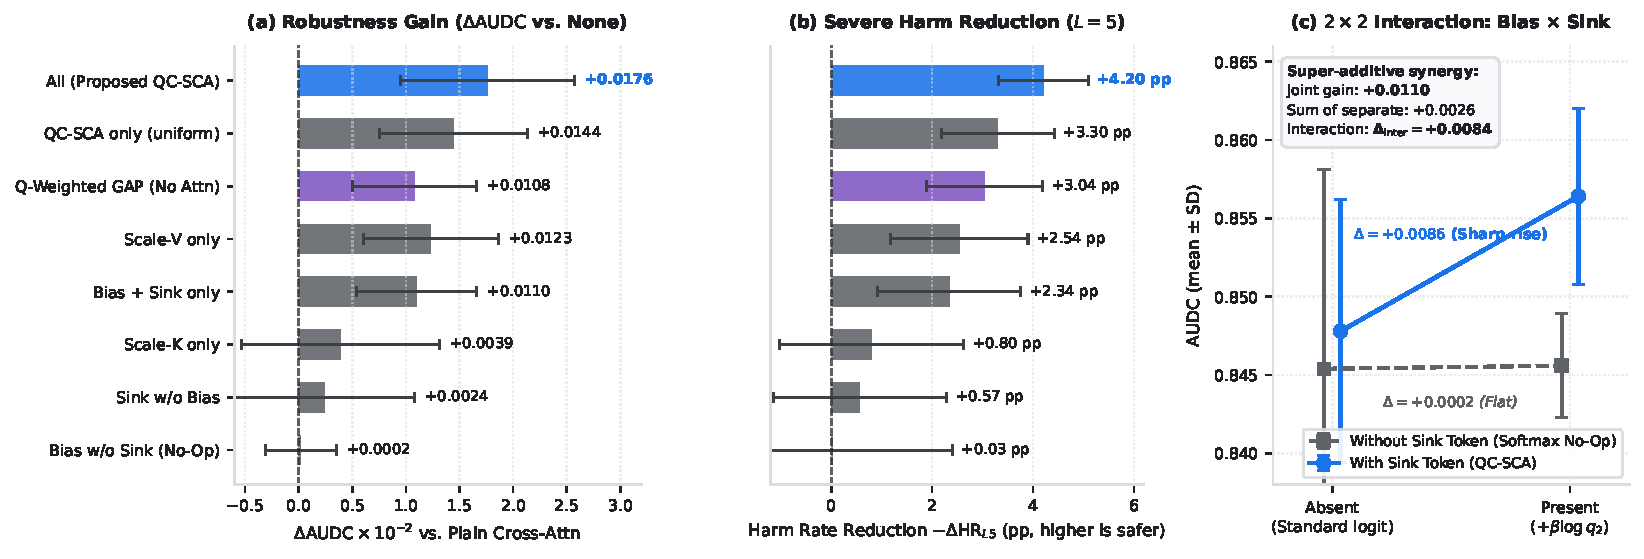
\includegraphics[width=\textwidth]{figures/fig7_ablation_partb.pdf}
\caption{Component ablation of the attention mechanism and sink token (Table~\ref{tab:ablation}, Part~B; mean $\pm$ standard deviation across seeds 42--44, $n=600$ test evaluations per configuration). 
(a)~Degradation robustness gain ($\Delta\text{AUDC} \times 10^{-2}$) relative to unmodulated cross-attention (\emph{None}, dashed vertical reference at zero). 
(b)~Harm Rate reduction ($-\Delta\text{HR}_{L5}$ in percentage points, pp; higher indicates a safer model) at the most severe degradation level ($L=5$). 
(c)~$2\times 2$ factorial interaction plot of Logit Bias $\times$ Sink Token on AUDC: without a sink token (dashed gray line), the quality bias is an exact softmax no-op ($\Delta = +0.0002$, flat); with a sink token (solid blue line), the quality bias takes effect ($\Delta = +0.0086$, sharp rise), consistent with a super-additive interaction ($\Delta_{\text{inter}} = +0.0084$; three seeds, not formally tested).}
\label{fig:ablation_partb}
\end{figure*}
The factorisation of Eq.~\eqref{eq:message_factorization} describes how the two mechanisms act on the message (Scale-V as a query-independent factor $q_2$, the sink as a query-dependent factor $g_i$) and is consistent with the ablation; it is a mechanistic description and not evidence that this difference causes the observed gains. Over all $n=21$ asymmetric evaluations ($3$ seeds $\times$ $7$ types), the full model has a higher AUDC than \emph{None} in every evaluation (all $21$ paired differences positive; exact two-sided Wilcoxon signed-rank $p = 2/2^{21} = 9.5\times10^{-7}$; mean $\Delta\text{AUDC} = +0.0176$) and a lower $\text{PFR}_{L5}$ ($-7.10$~pp). On clean test images the two models give identical absolute errors on $165$ of $200$ test pairs, leaving $n=35$ non-zero paired differences; a Wilcoxon test on these shows no significant difference ($W = 306.0$, nominal $p = 0.866$; $p \ge 0.090$ across all three ablation seeds). This agrees with the main clean benchmark, where the difference between Standard Cross-Attention and \qadfnet{} ($\Delta\kappa_w = +0.0105$) is not significant ($p_{\text{Holm}} = 0.7220$). Since the $21$ evaluations share seeds and test pairs, these $p$-values are nominal and descriptive.

\paragraph{Token grid (Part~C)} Across $G \in \{1,7,14,28\}$ ($N \in \{1,49,196,784\}$ tokens), all five metrics improve monotonically with $G$: $\kappa_w$ rises from $0.8583$ to $0.8846$, AUDC from $0.8416$ to $0.8687$, and $\text{HR}_{L5}$ falls from $19.12\%$ to $13.93\%$. The native output of the frozen EfficientNet-B4 is $14\times14$ (stride 32 at $448\times448$). For $G=28$ feature maps are taken from the penultimate stage (stride 16); $G=7$ is obtained by $2\times2$ average pooling and $G=1$ by GAP. Although the attention matrix grows $16\times$ (from $196^2=38{,}416$ to $784^2=614{,}656$ elements), peak VRAM increases by only $+11.9\%$ ($216.7 \to 242.5$\,MB) and latency by $+19.2\%$ ($28.7 \to 34.2$\,ms), because the frozen backbone passes dominate (Section~\ref{sec:r_backbone}). We keep $G=14$ as the default because it operates on the native backbone stage without tapping intermediate layers, keeps real-time throughput ($28.7$\,ms, $\approx 35$ FPS) and captures most of the safety gain: the Harm Rate and flip-rate gains show diminishing returns beyond $G=14$ ($\text{HR}_{L5}$: $-2.30$~pp for $G=7\to14$ vs.\ $-0.59$~pp for $14\to28$; $\text{PFR}_{L5}$: $-4.40$~pp vs.\ $-0.90$~pp), whereas the $\kappa_w$ gain does not ($+0.0066$ vs.\ $+0.0083$). Moving from $G=1$ to $G=14$ gives $88.6\%$ of the Harm Rate reduction reached at $G=28$. This choice is a cost--benefit decision, and $G=28$ is the better configuration on every metric. At $G=1$ and $G=7$ the full module is below the attention-free \emph{Q-Weighted GAP} of Part~B on all five metrics (e.g.\ AUDC $0.8416$ and $0.8523$ vs.\ $0.8562$); it exceeds it only from $G=14$ onwards. Moreover, $q_2$ is a per-image scalar, so the sink modulates queries according to cross-view affinity $Z_i$ and not according to a local quality map of View~2; spatially resolved quality maps $\mathbf{q}\in(0,1]^N$ are a natural extension.

\paragraph{Number of heads (Part~D)} With $d=128$ fixed, $\kappa_w$ rises from $0.8606$ ($H=1$) to $0.8653$ ($H=2$), $0.8763$ ($H=4$) and $0.8792$ ($H=8$), and $\text{HR}_{L5}$ falls from $18.48\%$ to $16.88\%$, $14.52\%$ and $14.12\%$. The difference between $H=4$ and $H=8$ ($+0.0029$ in $\kappa_w$, $-0.40$~pp in $\text{HR}_{L5}$) is smaller than the seed standard deviations ($0.0048$ and $0.89$~pp), so we cannot separate them and use $H=4$ as a compromise between capacity and per-head dimension. We did not analyse what individual heads attend to and make no claim about head specialisation.

\paragraph{Limitations of the ablation} (i)~The design is one-factor-at-a-time, not factorial: only the bias--sink contrast forms a complete $2\times2$ (without Scale-V), and \emph{Bias + Scale-V without sink} and \emph{Sink + Scale-V without bias} were not run. (ii)~Three seeds are used and several differences between neighbouring configurations are of the order of seed-to-seed variability. (iii)~The ablation degradation experiments use analytically attenuated quality scores, so Part~A does not test the estimator on degraded images; the online evaluation of Section~\ref{sec:r_online_fq} does not include the ablation variants. (iv)~All results are on a single dataset with $200$ test pairs from $100$ patients and ablation results are computed on the test set; they are used descriptively, not for model selection.

\subsection{Backbone variants and computational cost}
\label{sec:r_backbone}

We examine whether clean-image behaviour depends on the feature extractor, and what the fusion costs. Part~A of Table~\ref{tab:backbone_cost} repeats part of the clean-image comparison of Table~\ref{tab:main} with three frozen backbones (EfficientNet-B4, ConvNeXt-Tiny and Swin-Tiny) over five seeds (42--46). For each backbone it contains Single-View~V1, Concat, Standard Cross-Attention, Q-Weighted GAP and the proposed fusion in learned-$\hat q$ mode; the other baselines are not included. Part~B reports the cost of selected fusion variants on EfficientNet-B4. No significance tests were performed in this subsection.

\begin{table*}[!tb]
\centering
\renewcommand{\arraystretch}{0.7}
\caption{Backbone variants on the clean test set (Part~A; mean $\pm$ standard deviation over seeds 42--46, $\text{ddof}=0$; $n=200$ test pairs) and computational footprint (Part~B; batch size~1, FP32, one NVIDIA Tesla T4). ``\qcsca{} (Core Model)'' is the dual-view architecture with the proposed fusion; ``Full Pipeline'' adds the MobileNetV3-Small estimator $f_Q$ (two $224\times224$ inputs). Complexity was profiled with \texttt{thop} and is reported as GMACs and GFLOPs ($2\times$MACs). Bold marks the highest value per backbone and column. No significance tests were performed.}
\label{tab:backbone_cost}
\footnotesize
\setlength{\tabcolsep}{4pt}
\begin{tabular}{llcc}
\toprule
Backbone & Fusion Architecture & QWK ($\kappa_w$) & Accuracy \\
\midrule
\multicolumn{4}{l}{\textbf{Part A: Backbone variants (clean images)}} \\
\multirow{5}{*}{ConvNeXt-Tiny \citep{Liu2022convnext}}
  & Single-View V1        & $0.8681 \pm 0.0127$ & $69.10\% \pm 3.53\%$ \\
  & Concat                & $0.8850 \pm 0.0062$ & $71.20\% \pm 2.80\%$ \\
  & Standard Cross-Attn   & $0.8905 \pm 0.0082$ & $74.60\% \pm 2.01\%$ \\
  & Q-Weighted GAP        & $0.8950 \pm 0.0116$ & $75.40\% \pm 2.62\%$ \\
  & \qcsca{} (Proposed)   & $\mathbf{0.9009 \pm 0.0075}$ & $\mathbf{75.70\% \pm 2.58\%}$ \\
\midrule
\multirow{5}{*}{Swin-Tiny \citep{Liu2021swin}}
  & Single-View V1        & $0.8707 \pm 0.0160$ & $75.50\% \pm 2.35\%$ \\
  & Concat                & $0.8943 \pm 0.0147$ & $75.20\% \pm 3.17\%$ \\
  & Standard Cross-Attn   & $0.8958 \pm 0.0119$ & $\mathbf{77.30\% \pm 2.01\%}$ \\
  & Q-Weighted GAP        & $0.8968 \pm 0.0088$ & $76.40\% \pm 2.50\%$ \\
  & \qcsca{} (Proposed)   & $\mathbf{0.8988 \pm 0.0079}$ & $76.70\% \pm 2.99\%$ \\
\midrule
\multirow{5}{*}{EfficientNet-B4 \citep{Tan2019efficientnet}}
  & Single-View V1        & $0.8452 \pm 0.0143$ & $66.70\% \pm 2.36\%$ \\
  & Concat                & $0.8681 \pm 0.0086$ & $66.80\% \pm 3.33\%$ \\
  & Standard Cross-Attn   & $0.8700 \pm 0.0183$ & $67.10\% \pm 4.03\%$ \\
  & Q-Weighted GAP        & $0.8765 \pm 0.0075$ & $68.30\% \pm 1.75\%$ \\
  & \qcsca{} (Proposed)   & $\mathbf{0.8805 \pm 0.0102}$ & $\mathbf{68.70\% \pm 1.86\%}$ \\
\midrule
\multicolumn{4}{l}{\textbf{Part B: Computational complexity and inference footprint (EfficientNet-B4)}} \\
\multicolumn{2}{l}{Method} & Total Parameters / Comput. Cost & Latency / Peak GPU Memory \\
\midrule
\multicolumn{2}{l}{Average}                               & 17.78\,M / 25.4\,GFLOPs (12.7\,GMACs) & 27.0 $\pm$ 0.1\,ms / 216.2\,MB \\
\multicolumn{2}{l}{Concat}                                & 17.81\,M / 25.4\,GFLOPs (12.7\,GMACs) & 27.1 $\pm$ 0.1\,ms / 216.4\,MB \\
\multicolumn{2}{l}{Standard Cross-Attn}                   & 17.91\,M / 25.4\,GFLOPs (12.7\,GMACs) & 28.3 $\pm$ 0.1\,ms / 216.7\,MB \\
\multicolumn{2}{l}{\qcsca{} (Core Model)}                 & 17.91\,M / 25.4\,GFLOPs (12.7\,GMACs) & 28.7 $\pm$ 0.0\,ms / 216.7\,MB \\
\multicolumn{2}{l}{\qcsca{} (Full Pipeline w/ $f_Q$)}     & 20.45\,M / 25.7\,GFLOPs (12.8\,GMACs) & 30.8 $\pm$ 0.1\,ms / 238.5\,MB \\
\bottomrule
\end{tabular}
\end{table*}

\paragraph{Clean-image agreement across backbones} Among the five configurations compared, the proposed fusion has the highest QWK on each backbone, and the order Concat $<$ Standard Cross-Attention $<$ Q-Weighted GAP $<$ proposed fusion holds in all three cases; all fusion variants also exceed Single-View~V1. The margin of the proposed fusion over Standard Cross-Attention is $+0.0104$ on ConvNeXt-Tiny, $+0.0030$ on Swin-Tiny and $+0.0105$ on EfficientNet-B4, of the order of one seed-wise standard deviation ($0.0075$--$0.0183$) on the first and last and below one on Swin-Tiny ($0.0079$--$0.0119$). Accuracy is higher for the proposed fusion on ConvNeXt-Tiny ($+1.1$~pp) and EfficientNet-B4 ($+1.6$~pp) and lower on Swin-Tiny ($-0.6$~pp), all within seed-wise standard deviations ($1.9$--$4.0$~pp). The margin over Q-Weighted GAP is smaller still ($+0.0059$, $+0.0020$ and $+0.0040$ in $\kappa_w$; $+0.3$, $+0.3$ and $+0.4$~pp in accuracy) and below one seed-wise standard deviation of either method in every case. The three backbones share test pairs and seeds, so the consistent ordering is not independent evidence and is directional only. The ranking also holds only within this subset: on EfficientNet-B4, Co-Attention and Average Pooling reach a QWK at least as high as the proposed fusion (Table~\ref{tab:main}). We conclude that the module can be attached to the three backbones without a detectable loss of clean-image agreement relative to Standard Cross-Attention or Q-Weighted GAP. Robustness under degradation was evaluated with EfficientNet-B4 only, so these results do not show that the robustness and safety gains carry over to ConvNeXt-Tiny or Swin-Tiny.

\paragraph{Computational cost} Latency and peak GPU memory were measured on a single NVIDIA Tesla T4 at batch size~1 ($448\times448$, FP32) per dual-view pair, preceded by 50 warm-up iterations and averaged over 500 timed runs (where $\pm$ denotes standard deviation across runs); peak GPU memory was recorded using \texttt{torch.cuda.max\_memory\_allocated()}. Training was performed on the same GPU. Relative to Average Pooling, the proposed fusion adds $0.13$\,M parameters ($+0.7\%$) and $1.7$\,ms of latency ($28.7$ vs.\ $27.0$\,ms; $+6.3\%$). The parameters come from the cross-attention itself: Standard Cross-Attention and the proposed fusion have the same parameter count ($17.91$\,M) and peak memory ($216.7$\,MB), and the quality conditioning adds $0.4$\,ms ($28.7$ vs.\ $28.3$\,ms). According to \texttt{thop}, the frozen EfficientNet-B4 passes account for nearly all computation ($12.69$ of $12.71$\,GMACs, about $99.8\%$) and the fusion operator adds approximately $0.02$\,GMACs. Because \texttt{thop} profiles standard linear projections and omits attention score contractions, an analytical count for bidirectional multi-head attention adds $4 \times H \times N \times (N+1) \times d_h \approx 0.02$\,GMACs ($QK^T$ and $AV$ contractions across both directions, $4 \times 4 \times 196 \times 197 \times 32 \approx 1.98 \times 10^7$ MACs), bringing the complete fusion module to approximately $0.04$\,GMACs ($0.08$\,GFLOPs), about $0.3\%$ of the backbone's computation.
The quality estimator ($2.54$\,M parameters, $0.12$\,GMACs for both $224\times224$ views) is small in computation ($+0.9\%$ MACs relative to the core model) but not in parameters ($+14.2\%$), latency ($+2.1$\,ms, $+7.3\%$) or peak memory ($+21.8$\,MB, $+10.1\%$). The full pipeline requires $20.45$\,M parameters, $12.83$\,GMACs ($25.67$\,GFLOPs), $30.8$\,ms and $238.5$\,MB per examination. In the core model, varying the grid gives $27.8$\,ms / $216.3$\,MB for $G=7$, $28.7$\,ms / $216.7$\,MB for $G=14$ and $34.2$\,ms / $242.5$\,MB for $G=28$. CLAHE takes about $3.5$\,ms per pair on the host CPU and is not included; run sequentially, the end-to-end time is about $34$\,ms per examination ($\approx29$ examinations per second at batch size~1 on this hardware). Throughput on other hardware or with batching was not evaluated.

\subsection{Empirical check of the message bound}
\label{sec:r_prop1}

As a sanity check of Lemma~\ref{lem:1}, Table~\ref{tab:prop1} compares the measured $\ell_2$ norm of the cross-attention update with the bound $q_2 \cdot \max_j \|W_v \mathbf{f}_2^{(j)}\|_2$ for clean test samples. Because the lemma follows from Eq.~\eqref{eq:attn_update}, a ratio at or below $1$ is expected by construction; the check mainly verifies the implementation. Because the uncorrupted test cohort has high average image quality ($\bar{q} \approx 0.88\text{--}0.91$) where the majority of pairs lie at $q_2 > 0.75$, a diagnostic batch of 15 test pairs was purposively sampled to enrich the lower-quality tail of the available natural distribution ($n=9$ in $(0.50, 0.75]$ and $n=6$ in $(0.75, 1.00]$), ensuring that the quality-attenuation factor is non-trivial during the check.

\begin{table}[!tb]
\centering
\renewcommand{\arraystretch}{0.7}
\caption{Measured cross-attention update norm divided by the bound of Lemma~\ref{lem:1}, per quality interval of $q_2$ (clean test samples). A ratio $\le 1.0$ is consistent with the lemma.}
\label{tab:prop1}
\small
\adjustbox{max width=\columnwidth}{%
\begin{tabular}{lccccc}
\toprule
$q_2$ interval & Samples & Mean ratio & Max ratio & 95th pct. & Ratio $\le 1.0$ \\
\midrule
$(0.50, 0.75]$ & 9 & 0.4378 & 0.4635 & 0.4608 & 100\% \\
$(0.75, 1.00]$ & 6 & 0.4204 & 0.4645 & 0.4535 & 100\% \\
\bottomrule
\end{tabular}}
\end{table}

The ratio never exceeds $0.4645$ in these $15$ samples, confirming that the implementation respects the bound with substantial slack. However, because natural uncorrupted pairs contain virtually no images with $q_2 < 0.50$ (Section~\ref{sec:r_safety}), this check does not directly probe the strongly degraded regime ($q_2 \le 0.50$) under synthetic corruption, which remains an empirical limitation of this sanity check. Instead, the attention-mass measurements under synthetic degradation in Section~\ref{sec:r_safety} (sink mass up to $0.49$ and compound factor $\approx0.045$ at Level~5) provide the complementary empirical evidence on the behaviour of the module under severe quality degradation.

%%=================================================================
%%  SECTION 6 --- DISCUSSION
%%=================================================================
\section{Discussion}
\label{sec:discussion}

\paragraph{Principal findings} Four findings emerge. First, on clean data the fusion strategies are hard to separate: \qadfnet{} is on par with Average Pooling, Q-Weighted GAP and Co-Attention, and quality conditioning has no detectable clean-image cost. Second, when one view degrades, \qadfnet{} limits the growth of the fused model's disagreement with the clearer single view: its Harm Rate grows by $2.19$~pp from clean to the most severe level under the controlled benchmark, against $5.79$--$16.29$~pp for the five fusion baselines of Table~\ref{tab:harm_flip}, with a parallel pattern in prediction flips and feature drift. The AUDC advantage over Average and Concat survives multiplicity correction, while that over Cross-Attention, Co-Attention and Max-Pooling points in the same direction; the AUDC ranking of the five methods reported is the same when the quality scores are estimated online from the degraded images, and \qadfnet{} again has the smallest Level-5 Harm Rate (Table~\ref{tab:online_fq_benchmark}; descriptive, without tests). Third, the ablation agrees with the invariance argument: a quality bias without a sink behaves like no bias, a sink without the bias gives only small changes, and the two together reduce Harm Rate and flip rate. Fourth, quality weighting itself accounts for much of the benefit: Q-Weighted GAP, which has no attention, captures about half of the AUDC gain of \qadfnet{} over Cross-Attention in the five-seed benchmark, but is numerically below the full spatial attention module under both analytical attenuation and online estimation, by margins of the order of one seed-wise standard deviation.

\paragraph{What the ablation does and does not show} In our data, access to quality information matters more than the particular route by which it enters the model. Scale-V alone (AUDC $0.8577$), bias plus sink ($0.8564$) and quality-weighted pooling without any attention ($0.8562$) lie within $0.0015$ of each other, and each recovers most of the improvement of the full model over plain cross-attention ($0.8630$ vs.\ $0.8454$). A simple reading is that a quality signal must reach the value path or the consensus weights, or be given a place to leave the softmax, and that each route is sufficient to obtain most of the benefit on this dataset. The bias--sink contrast supports the invariance argument: the logit-bias route works only together with the sink, since neither factor alone moves the metrics beyond seed variability. What the data do not show is that the full spatial module adds much beyond simple quality weighting. Its advantage over Q-Weighted GAP is $+0.0068$ AUDC and $-1.16$~pp $\text{HR}_{L5}$ in the ablation and $+0.0082$ AUDC in the five-seed benchmark, of the order of one seed-wise standard deviation and untested, and at $G=1$ and $G=7$ the module is below Q-Weighted GAP. The spatial formulation therefore pays off here only from $G=14$ onwards, and a larger grid performs better still. The additional value of the sink lies in the query-dependent factor $g_i$ and in the visible redistribution of attention mass; the data do not demonstrate that this adds much beyond Scale-V or quality-weighted pooling.

\paragraph{Clinical implications} A dual-view screening system is useful only if it does not make decisions worse than the clearer photograph would. The Harm Rate and flip-rate analyses give a concrete way to audit this, and show that unconditioned fusion can fall below quality-based view selection in two of the three view scenarios (Table~\ref{tab:degrad_scenarios}). Quality-conditioned fusion is complementary to, and does not replace, acquisition quality control: severely ungradable images should still be recaptured or referred. On the natural DeepDRiD test pairs, which contain almost no severely degraded views, \qadfnet{} was neither better nor worse than the baselines in Harm Rate; any benefit in routine data should therefore be expected to be small, and the mechanism is most relevant where acquisition quality is variable, such as tele-screening or non-mydriatic settings. We have not tested these settings.

\paragraph{Limitations}
\begingroup
\renewcommand{\labelenumi}{(\roman{enumi})}
\begin{enumerate}
  \item The main benchmark supplies analytically attenuated quality scores to isolate the fusion mechanism. The end-to-end evaluation of Section~\ref{sec:r_online_fq} applies $f_Q$ to the degraded images and gives similar results ($\text{AUDC} = 0.8662$, $\text{HR}_{L5} = 14.63\%$), but it covers five methods, is descriptive, and uses degradations whose strength was calibrated against the same estimator; it therefore does not show that $f_Q$ is reliable on other corruptions or on real acquisitions, and external validation on uncurated multi-centre cohorts remains essential.
  \item Degradations are synthetic and applied to one view of otherwise good pairs; real asymmetries may be more complex.
  \item Evidence comes from one public dataset with $100$ test patients, a single frozen backbone for the degradation experiments and five (three for ablations) training seeds; there is no external validation.
  \item The per-image scalar $q$ cannot represent partially degraded views, which may explain the weaker results under glare and occlusion (see qualitative demonstration in Fig.~\ref{fig:qualitative_cases}b).
  \item Harm Rate uses a privileged reference view selected with quality information; its absolute values depend on this choice, and Level-0 values reflect disagreement between independently trained models.
  \item While the quality estimator was verified against expert scores across the full clean test cohort ($\rho = 0.7967$, $n=400$ images; Section~\ref{sec:degradation}), its outputs on degraded images were examined only through their empirical mean progression per degradation type, not against direct expert ratings under synthetic corruption.
  \item Apart from Q-Weighted GAP and the oracle Best-Single reference, baselines receive no quality information, and no uncertainty-weighted or other learned quality-aware fusion operator was compared.
  \item Q-Weighted GAP is evaluated across degradation types in Table~\ref{tab:degrad_summary}, across view scenarios in Table~\ref{tab:degrad_scenarios}, in the ablation study (Table~\ref{tab:ablation}) and across severity levels under online quality estimation (Table~\ref{tab:online_fq_benchmark}), but it is omitted from the controlled analytic safety progression of Table~\ref{tab:harm_flip}, and no paired bootstrap significance test was conducted against it under the analytic benchmark. The Holm--Bonferroni multiplicity corrections in Sections~\ref{sec:r_degrad} and~\ref{sec:r_safety} are therefore formally defined over the family of five unconditioned fusion baselines, and evaluating Q-Weighted GAP within a unified paired testing framework remains a limitation.
  \item Many comparisons are not significant after correction, and seed-level and run-level tests describe training variability only.
\end{enumerate}
\endgroup

\paragraph{Future work} Natural next steps include replacing the scalar $q$ by a spatial quality map to handle localised occlusions and glare (as illustrated by the failure mode in Fig.~\ref{fig:qualitative_cases}b); comparing against further learned quality-aware baselines such as uncertainty-weighted fusion; measuring the sensitivity of the fusion to errors in $\hat q$, including on corruptions not used to calibrate $f_Q$; and validating the complete pipeline on external dual-view fundus datasets with real-world quality asymmetry and across additional modern backbones.

%%=================================================================
%%  SECTION 7 --- CONCLUSION
%%=================================================================
\section{Conclusion}
\label{sec:conclusion}

We studied quality asymmetry in dual-view diabetic retinopathy grading and showed that a per-image quality bias on attention logits is cancelled by the softmax. QADF-Net makes the bias effective with a zero-value sink token, combines it with quality-proportional value scaling in a spatial cross-attention module, and adds 0.13\,M parameters and 1.7\,ms per pair. On DeepDRiD it matched the strongest fusion baselines on clean images. When one view was degraded and quality scores were supplied analytically, it showed the smallest growth of Harm Rate, prediction flips and feature drift among the fusion baselines evaluated; when the scores were estimated online from the degraded images, it again had the highest AUDC and the lowest Level-5 Harm Rate among the five methods reported. Quality-weighted pooling without attention obtained a large part of this benefit, and the margin of the full module over it was of the order of one seed-wise standard deviation. The advantage was confined to moderate and high severity and was not visible on natural pairs. We regard QADF-Net and the accompanying Harm Rate protocol as a basis for safety-oriented evaluation of multi-view fundus fusion; validation on external datasets with real quality asymmetry is the main next step.

%%---------------------------------------------------------------
%%  BACK MATTER
%%---------------------------------------------------------------

\section*{CRediT authorship contribution statement}
\textbf{Quoc Thai Mai}: Conceptualization, Methodology, Software,
Formal analysis, Investigation, Data curation, Visualization,
Project administration, Writing -- original draft,
Writing -- review \& editing.
\textbf{Thanh Tuan Nguyen}: Supervision, Validation,
Writing -- review \& editing.
\textbf{Thi-The Phan}: Formal analysis, Resources,
Writing -- review \& editing.

\section*{Declaration of competing interest}
The authors declare that they have no known competing financial interests
or personal relationships that could have appeared to influence the work
reported in this paper.

\section*{Acknowledgements}
The authors would like to thank Ho Chi Minh City University of Technology and Engineering (HCMUTE) for providing computational resources to support this research.

\section*{Funding}
This research received no specific grant from funding agencies in the
public, commercial, or not-for-profit sectors.

\section*{Ethics statement}
This study uses the publicly available DeepDRiD dataset
\citep{Liu2022deepdrid}, which was collected under institutional ethical
approval with informed patient consent as documented by the original
dataset authors. No additional patient data were collected.

\section*{Data availability}
The DeepDRiD dataset is available through the challenge platform
described in \citet{Liu2022deepdrid}. Processed experimental results
will be deposited in a public repository upon acceptance.

\section*{Code availability}
Source code and pre-trained weights will be made publicly available
upon acceptance.



%%=================================================================
%%  APPENDICES
%%=================================================================
\appendix

%%---------------------------------------------------------------
%%  APPENDIX A --- NOTATION
%%---------------------------------------------------------------
\section{List of Symbols}
\label{app:notation}

\begin{table*}[!tb]
\centering
\caption{Mathematical notation used throughout the paper.}
\label{tab:notation}
\footnotesize
\begin{tabular}{ll}
\toprule
Symbol & Definition \\
\midrule
$I_1, I_2$             & Input fundus images (macula-centred / disc-centred view) \\
$q_1, q_2 \in (0,1]$   & Per-view quality scores (frozen estimator, oracle, analytic attenuation or constant) \\
$q^{\text{human}}$     & Expert quality score (Eq.~\ref{eq:qhuman}) \\
$\hat{q}$              & Quality score predicted by the estimator $f_Q$ \\
$G$                    & Token grid size ($G=14$ by default) \\
$N = G^2$              & Number of spatial tokens per view ($N=196$) \\
$d, d_h, H$            & Token dimension ($128$), per-head dimension, number of heads ($4$) \\
$\mathbf{f}_m^{(j)}$   & $j$-th spatial token of view $m$, dimension $d$ \\
$W_q, W_k, W_v, W_o$   & Query / key / value / output projection matrices \\
$k_{\text{sink}}$      & Learned key of the sink token \\
$v_{\text{sink}}$      & Value of the sink token, fixed to $\mathbf{0}$ \\
$\tau_{\text{sink}}$   & Sink token $(k_{\text{sink}}, v_{\text{sink}})$ \\
$\beta$                & Learnable scale of the quality logit bias \\
$\alpha_{ij}$, $\alpha_{i,\text{sink}}$ & Attention weights of query $i$ on token $j$ / on the sink \\
$g_i(q_2)$             & Fraction of attention mass kept on genuine tokens, $1-\alpha_{i,\text{sink}}$ \\
$\Attn{i}$             & Cross-view message received by query $i$ \\
$\mathbf{f}_{\text{cons}}$ & Consensus representation fed to the CORAL head \\
$\kappa_w$             & Quadratic weighted kappa (QWK) \\
$\mathrm{AUDC}$        & Area under the degradation curve \\
$L \in \{0,\ldots,5\}$ & Degradation severity (0 = clean) \\
$\text{Harm Rate}$, $\text{Help Rate}$ & Share of pairs where fusion is worse / better than the quality-selected view \\
$\mathrm{PFR}$, $\mathrm{FDI}$ & Prediction Flip Rate, Feature Drift Index \\
\bottomrule
\end{tabular}
\end{table*}

%%---------------------------------------------------------------
%%  APPENDIX B --- PROOF: BIAS-ALONE IS A SOFTMAX NO-OP
%%---------------------------------------------------------------
\section{\texorpdfstring{Proof of Remark~\ref{rem:noop}: invariance of a per-image quality bias}{Proof of the softmax invariance of a per-image quality bias}}
\label{app:noopproof}

Let $s^{0}_{ij} = Q_1^{(i)} (K_2^{(j)})^\top/\sqrt{d_h}$ be the unbiased logit between query $i$ and key $j\in\{1,\dots,N\}$, and let $c(q_2) = |\beta|\log q_2$ be a bias added to every key. The biased attention weight is
\begin{equation}
\begin{split}
  \tilde{\alpha}_{ij} &= \frac{\exp(s^{0}_{ij} + c(q_2))}{\sum_{k=1}^N \exp(s^{0}_{ik} + c(q_2))} \\
  &= \frac{\exp(c(q_2))\,\exp(s^{0}_{ij})}{\exp(c(q_2))\sum_{k=1}^N \exp(s^{0}_{ik})} \\
  &= \frac{\exp(s^{0}_{ij})}{\sum_{k=1}^N \exp(s^{0}_{ik})} = \alpha_{ij},
\end{split}
\end{equation}
for all $i,j$. Here $\exp(c(q_2)) = q_2^{|\beta|}>0$ does not depend on the key index, so it factors out of numerator and denominator. The attention distribution is therefore independent of $q_2$.

\paragraph{Role of the sink token} The cancellation occurs because the normalising sum runs over exactly the set of tokens that receive the bias. If the key set is augmented by a sink with logit $s_{i,\text{sink}}$ that does \emph{not} receive the bias, the denominator becomes
\begin{equation}
  D_i = \exp(s_{i,\text{sink}}) + q_2^{|\beta|} \sum_{k=1}^N \exp(s^{0}_{ik}),
\end{equation}
and $q_2^{|\beta|}$ can no longer be factored out. As $q_2 \to 0$, $q_2^{|\beta|} \to 0$, so $\alpha_{ij} \to 0$ for every genuine token and $\alpha_{i,\text{sink}} \to 1$. Because $v_{\text{sink}} = \mathbf{0}$, the message then contracts to zero.

%%---------------------------------------------------------------
%%  APPENDIX C --- FULL DEGRADATION RESULTS
%%---------------------------------------------------------------
\section{Full degradation benchmark results}
\label{app:fulldegrad}

Table~\ref{tab:s1_audc} gives the AUDC of the nine baselines and \qadfnet{} for each of the seven degradation types under asymmetric degradation (View~2 degraded, View~1 clean).

\begin{table*}[!tb]
\centering
\renewcommand{\arraystretch}{0.7}
\caption{AUDC for all methods and degradation types under asymmetric degradation (View~2 degraded, View~1 clean). Bold indicates the highest value per column among the fusion methods and \qadfnet{}.}
\label{tab:s1_audc}
\footnotesize
\adjustbox{max width=\textwidth}{%
\begin{tabular}{lccccccc}
\toprule
Method & Gaussian blur & Defocus blur & Motion blur & JPEG & Darkness & Glare & Occlusion \\
\midrule
Single-View V1        & 0.8452 & 0.8452 & 0.8452 & 0.8452 & 0.8452 & 0.8452 & 0.8452 \\
Single-View V2        & 0.5800 & 0.6331 & 0.6114 & 0.5718 & 0.7941 & 0.6307 & 0.8263 \\
Best-Single (Quality Selector)& 0.8553 & 0.8553 & 0.8553 & 0.8523 & 0.8650 & 0.8559 & 0.8607 \\
Concat                & 0.7959 & 0.8237 & 0.8165 & 0.8042 & 0.8473 & 0.8254 & 0.8581 \\
Average Pooling       & 0.8090 & 0.8292 & 0.8143 & 0.8294 & 0.8639 & 0.8469 & 0.8731 \\
Max-Pooling           & 0.8271 & 0.8434 & 0.8382 & 0.8347 & 0.8644 & 0.8439 & 0.8676 \\
Cross-Attention       & 0.8367 & 0.8443 & 0.8382 & 0.8406 & 0.8687 & 0.8594 & 0.8712 \\
Q-Weighted GAP        & 0.8482 & 0.8514 & 0.8506 & 0.8528 & 0.8745 & 0.8635 & 0.8678 \\
Co-Attention          & 0.8346 & 0.8467 & 0.8474 & 0.8369 & 0.8732 & 0.8680 & \textbf{0.8823} \\
\midrule
\textbf{\qadfnet{} (Proposed)}& \textbf{0.8599} & \textbf{0.8598} & \textbf{0.8609} & \textbf{0.8645} & \textbf{0.8795} & \textbf{0.8682} & 0.8732 \\
\bottomrule
\end{tabular}}
\end{table*}

%%---------------------------------------------------------------
%%  APPENDIX D --- HYPERPARAMETERS (TABLE S7)
%%---------------------------------------------------------------
\section{Hyperparameter and experimental configuration}
\label{app:config}

Table~\ref{tab:s7_config} summarises hyperparameters and the training environment for reproducibility.

\begin{table*}[!tb]
\centering
\caption{Experimental configuration and reproducibility specifications.}
\label{tab:s7_config}
\footnotesize
\begin{tabular}{@{}>{\raggedright\arraybackslash}p{0.22\textwidth}>{\raggedright\arraybackslash}p{0.74\textwidth}@{}}
\toprule
Parameter & Value \\
\midrule
Backbone & EfficientNet-B4 (default), ConvNeXt-Tiny or Swin-Tiny; pretrained and frozen; shared between views \\
Tokenisation & Shared $1\times1$ convolution and adaptive average pooling to $G\times G$ tokens ($G=14$, $N=196$, $d=128$); learned 2-D positional and view embeddings \\
Fusion module & Bidirectional QC-SCA, $H=4$ heads ($d_h=32$), residual connection and LayerNorm; learnable $\beta$ and sink key $k_{\text{sink}}$, $v_{\text{sink}}\equiv\mathbf{0}$, $\epsilon=10^{-6}$ \\
Quality estimator & MobileNetV3-Small (2.54\,M parameters), $224\times224$ input, loss $\mathcal{L}_{\text{MSE}}+0.5\,\mathcal{L}_{\text{rank}}$, AdamW (learning rate $5\times10^{-4}$, weight decay $10^{-4}$), batch size 16, 15 epochs, training partition only, frozen after training \\
Classifier head and loss & Monotonic CORAL head ($K-1=4$ thresholds), multi-threshold binary cross-entropy \\
Optimiser & AdamW (learning rate $3\times10^{-4}$, weight decay $10^{-4}$) \\
Schedule & Cosine annealing over 60 epochs, 5 warm-up epochs, $\eta_{\min}=10^{-6}$ \\
Batch size & 8 pairs $\times$ 4 accumulation steps = 32 pairs (64 photographs) \\
Model selection & Checkpoint with the highest validation QWK over 60 epochs (patient-stratified validation split) \\
Preprocessing & Bicubic resize to $448\times448$; CLAHE on the Lab luminance channel (clip limit 2.0, $8\times8$ grid) \\
Augmentation & Random resized crop (scale $[0.75,1.0]$, aspect ratio $[0.9,1.1]$), horizontal and vertical flips ($p=0.5$), rotation up to $\pm30^\circ$, colour jitter (brightness 0.3, contrast 0.35, saturation 0.25, hue 0.05), random greyscale ($p=0.1$) \\
Seeds & 42--46 (main benchmark); 42--44 (ablations) \\
Statistics & Patient-clustered bootstrap, $B=2{,}000$; Holm--Bonferroni correction at $\alpha=0.05$ \\
Software and hardware & PyTorch 2.x, timm 1.0.27; automatic mixed precision (FP16) for training; single NVIDIA Tesla T4 GPU (training and latency measurement) \\
Patient split audit & SHA-256 verified zero-leakage manifest \\
\bottomrule
\end{tabular}
\end{table*}

%%---------------------------------------------------------------
%%  APPENDIX E --- ONLINE QUALITY ESTIMATOR DEGRADATION BREAKDOWN
%%---------------------------------------------------------------
\section{Per-degradation performance under online quality estimation \texorpdfstring{($f_Q$)}{(f\_Q)}}
\label{app:online_fq_types}

Table~\ref{tab:s8_online_fq_types} provides the degradation-specific Level-5 diagnostic agreement ($\kappa_w$) and the empirically estimated quality score $\bar{q}_2$ for each of the seven degradation types under the online $f_Q$ evaluation of Section~\ref{sec:r_online_fq} (mean over five seeds, with seed-to-seed standard deviations ranging from $0.008$ to $0.022$ for \qadfnet{} and $0.003$ to $0.087$ across the baselines). The Overall Mean row represents the unweighted mean across the seven degradation categories.

\begin{figure*}[!tb]
\centering
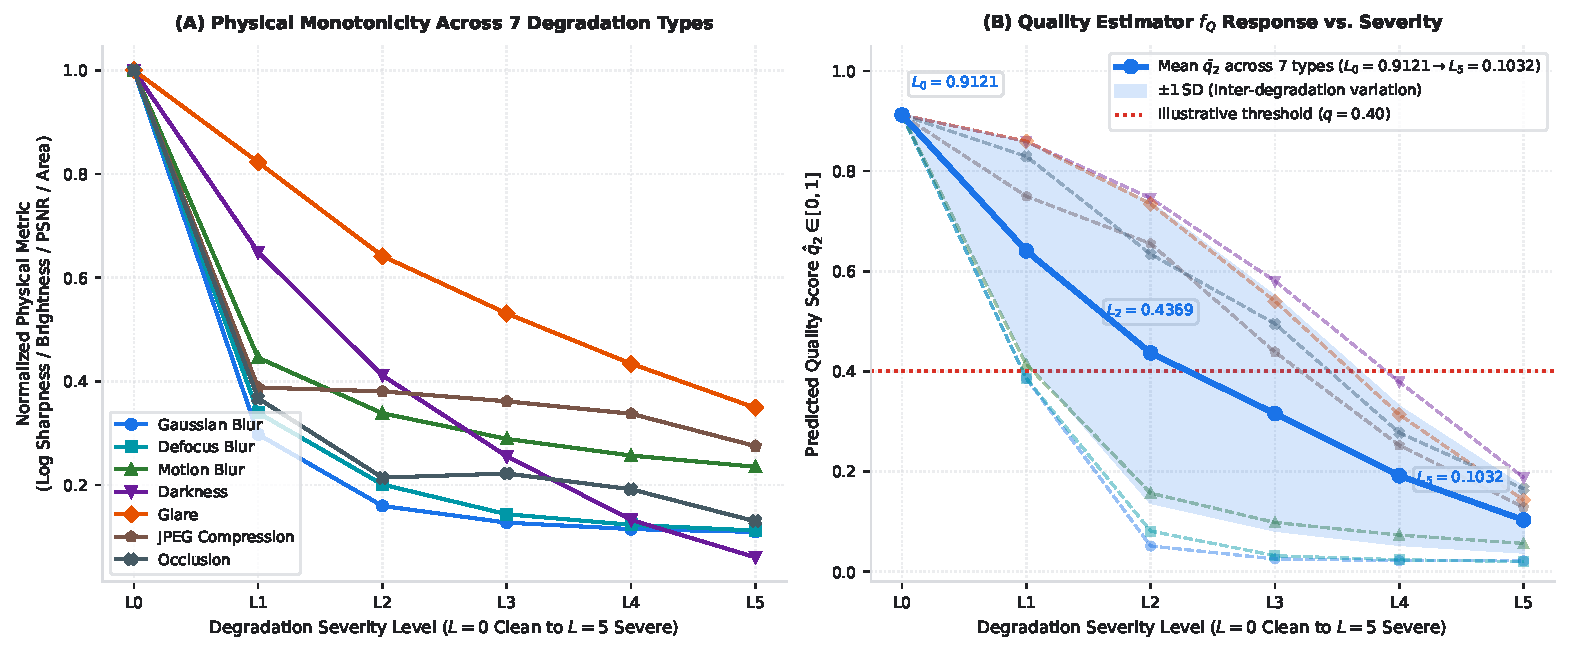
\includegraphics[width=0.9\textwidth]{figures/fig_s1_degradation_calibration.pdf}
\caption{Controlled degradation calibration and quality score response curves across severity levels $L=0$ to $L=5$. 
(A)~Physical monotonicity profiles across all seven degradation types showing normalised physical metrics (logarithmic sharpness for Gaussian/Defocus/Motion blur, inverse brightness for Glare, linear brightness for Darkness, PSNR for JPEG compression, and unoccluded retinal area for Occlusion). 
(B)~Empirical quality response of the frozen MobileNetV3 quality estimator $f_Q$ across severity levels (blue solid line: cohort mean $\bar{q}_2$ averaged across all $n=200$ test pairs, five seeds and seven degradation categories, exactly reproducing the reported cohort trajectory: $L_0=0.9121$, $L_1=0.6406$, $L_2=0.4369$, $L_3=0.3157$, $L_4=0.1916$, and $L_5=0.1032$; shaded band: $\pm 1\,\text{SD}$ inter-degradation variation across the seven categories; dashed curves: individual degradation trajectories; dotted red reference: illustrative low-quality threshold at $q=0.40$, display only).}
\label{fig:calibration_curves}
\end{figure*}

\begin{table*}[!tb]
\centering
\renewcommand{\arraystretch}{0.7}
\caption{Diagnostic agreement ($\kappa_w$) at severe degradation ($L=5$) and mean estimated quality score $\bar{q}_2$ across seven degradation types under online $f_Q$ estimation (mean over five seeds; asymmetric scenario, View~2 degraded). $\bar q_2$ is the mean estimated quality of View~2 over test pairs and seeds. The best value per row is in bold.}
\label{tab:s8_online_fq_types}
\footnotesize
\begin{tabular}{l ccccc c}
\toprule
\textbf{Degradation Type} & \textbf{Concat} & \textbf{Average} & \textbf{Cross-Attn} & \textbf{Q-W.\ GAP} & \textbf{\qadfnet{}} & \textbf{Estimated $\bar{q}_2(L5)$} \\
\midrule
Gaussian Blur    & 0.6810 & 0.7222 & 0.8173 & 0.8321 & \textbf{0.8529} & 0.0215 \\
Defocus Blur     & 0.7464 & 0.7504 & 0.8159 & 0.8321 & \textbf{0.8542} & 0.0202 \\
Motion Blur      & 0.7562 & 0.7722 & 0.8033 & 0.8251 & \textbf{0.8529} & 0.0564 \\
JPEG Compression & 0.7058 & 0.7580 & 0.8240 & 0.8353 & \textbf{0.8505} & 0.1284 \\
Darkness         & 0.7430 & 0.7904 & 0.8387 & 0.8500 & \textbf{0.8652} & 0.1878 \\
Glare            & 0.7596 & 0.7902 & 0.8116 & 0.8281 & \textbf{0.8510} & 0.1429 \\
Occlusion        & 0.8510 & 0.8598 & 0.8642 & 0.8633 & \textbf{0.8664} & 0.1654 \\
\midrule
\textbf{Overall Mean ($L5$)} & 0.7490 & 0.7776 & 0.8250 & 0.8380 & \textbf{0.8562} & 0.1032 \\
\bottomrule
\end{tabular}
\end{table*}

%%---------------------------------------------------------------
%%  BIBLIOGRAPHY
%%---------------------------------------------------------------
\bibliographystyle{elsarticle-harv}
\bibliography{refs_cmig}


\end{document}
\endinput